%  LaTeX support: latex@mdpi.com 
%  For support, please attach all files needed for compiling as well as the log file, and specify your operating system, LaTeX version, and LaTeX editor.

%=================================================================
\documentclass[mathematics,article,submit,pdftex,moreauthors]{Definitions/mdpi} 
 
%--------------------
% Class Options:
%--------------------
%----------
% journal
%----------
% Choose between the following MDPI journals:
% acoustics, actuators, addictions, admsci, adolescents, aerobiology, aerospace, agriculture, agriengineering, agrochemicals, agronomy, ai, air, algorithms, allergies, alloys, analytica, analytics, anatomia, animals, antibiotics, antibodies, antioxidants, applbiosci, appliedchem, appliedmath, applmech, applmicrobiol, applnano, applsci, aquacj, architecture, arm, arthropoda, arts, asc, asi, astronomy, atmosphere, atoms, audiolres, automation, axioms, bacteria, batteries, bdcc, behavsci, beverages, biochem, bioengineering, biologics, biology, biomass, biomechanics, biomed, biomedicines, biomedinformatics, biomimetics, biomolecules, biophysica, biosensors, biotech, birds, bloods, blsf, brainsci, breath, buildings, businesses, cancers, carbon, cardiogenetics, catalysts, cells, ceramics, challenges, chemengineering, chemistry, chemosensors, chemproc, children, chips, cimb, civileng, cleantechnol, climate, clinpract, clockssleep, cmd, coasts, coatings, colloids, colorants, commodities, compounds, computation, computers, condensedmatter, conservation, constrmater, cosmetics, covid, crops, cryptography, crystals, csmf, ctn, curroncol, cyber, dairy, data, ddc, dentistry, dermato, dermatopathology, designs, devices, diabetology, diagnostics, dietetics, digital, disabilities, diseases, diversity, dna, drones, dynamics, earth, ebj, ecologies, econometrics, economies, education, ejihpe, electricity, electrochem, electronicmat, electronics, encyclopedia, endocrines, energies, eng, engproc, entomology, entropy, environments, environsciproc, epidemiologia, epigenomes, est, fermentation, fibers, fintech, fire, fishes, fluids, foods, forecasting, forensicsci, forests, foundations, fractalfract, fuels, future, futureinternet, futurepharmacol, futurephys, futuretransp, galaxies, games, gases, gastroent, gastrointestdisord, gels, genealogy, genes, geographies, geohazards, geomatics, geosciences, geotechnics, geriatrics, grasses, gucdd, hazardousmatters, healthcare, hearts, hemato, hematolrep, heritage, higheredu, highthroughput, histories, horticulturae, hospitals, humanities, humans, hydrobiology, hydrogen, hydrology, hygiene, idr, ijerph, ijfs, ijgi, ijms, ijns, ijpb, ijtm, ijtpp, ime, immuno, informatics, information, infrastructures, inorganics, insects, instruments, inventions, iot, j, jal, jcdd, jcm, jcp, jcs, jcto, jdb, jeta, jfb, jfmk, jimaging, jintelligence, jlpea, jmmp, jmp, jmse, jne, jnt, jof, joitmc, jor, journalmedia, jox, jpm, jrfm, jsan, jtaer, jvd, jzbg, kidneydial, kinasesphosphatases, knowledge, land, languages, laws, life, liquids, literature, livers, logics, logistics, lubricants, lymphatics, machines, macromol, magnetism, magnetochemistry, make, marinedrugs, materials, materproc, mathematics, mca, measurements, medicina, medicines, medsci, membranes, merits, metabolites, metals, meteorology, methane, metrology, micro, microarrays, microbiolres, micromachines, microorganisms, microplastics, minerals, mining, modelling, molbank, molecules, mps, msf, mti, muscles, nanoenergyadv, nanomanufacturing,\gdef\@continuouspages{yes}} nanomaterials, ncrna, ndt, network, neuroglia, neurolint, neurosci, nitrogen, notspecified, %%nri, nursrep, nutraceuticals, nutrients, obesities, oceans, ohbm, onco, %oncopathology, optics, oral, organics, organoids, osteology, oxygen, parasites, parasitologia, particles, pathogens, pathophysiology, pediatrrep, pharmaceuticals, pharmaceutics, pharmacoepidemiology,\gdef\@ISSN{2813-0618}\gdef\@continuous pharmacy, philosophies, photochem, photonics, phycology, physchem, physics, physiologia, plants, plasma, platforms, pollutants, polymers, polysaccharides, poultry, powders, preprints, proceedings, processes, prosthesis, proteomes, psf, psych, psychiatryint, psychoactives, publications, quantumrep, quaternary, qubs, radiation, reactions, receptors, recycling, regeneration, religions, remotesensing, reports, reprodmed, resources, rheumato, risks, robotics, ruminants, safety, sci, scipharm, sclerosis, seeds, sensors, separations, sexes, signals, sinusitis, skins, smartcities, sna, societies, socsci, software, soilsystems, solar, solids, spectroscj, sports, standards, stats, std, stresses, surfaces, surgeries, suschem, sustainability, symmetry, synbio, systems, targets, taxonomy, technologies, telecom, test, textiles, thalassrep, thermo, tomography, tourismhosp, toxics, toxins, transplantology, transportation, traumacare, traumas, tropicalmed, universe, urbansci, uro, vaccines, vehicles, venereology, vetsci, vibration, virtualworlds, viruses, vision, waste, water, wem, wevj, wind, women, world, youth, zoonoticdis 
% For posting an early version of this manuscript as a preprint, you may use "preprints" as the journal. Changing "submit" to "accept" before posting will remove line numbers.

%---------
% article
%---------
% The default type of manuscript is "article", but can be replaced by: 
% abstract, addendum, article, book, bookreview, briefreport, casereport, comment, commentary, communication, conferenceproceedings, correction, conferencereport, entry, expressionofconcern, extendedabstract, datadescriptor, editorial, essay, erratum, hypothesis, interestingimage, obituary, opinion, projectreport, reply, retraction, review, perspective, protocol, shortnote, studyprotocol, systematicreview, supfile, technicalnote, viewpoint, guidelines, registeredreport, tutorial
% supfile = supplementary materials

%----------
% submit
%----------
% The class option "submit" will be changed to "accept" by the Editorial Office when the paper is accepted. This will only make changes to the frontpage (e.g., the logo of the journal will get visible), the headings, and the copyright information. Also, line numbering will be removed. Journal info and pagination for accepted papers will also be assigned by the Editorial Office.

%------------------
% moreauthors
%------------------
% If there is only one author the class option oneauthor should be used. Otherwise use the class option moreauthors.

%---------
% pdftex
%---------
% The option pdftex is for use with pdfLaTeX. Remove "pdftex" for (1) compiling with LaTeX & dvi2pdf (if eps figures are used) or for (2) compiling with XeLaTeX.

%=================================================================
% MDPI internal commands - do not modify
\firstpage{1} 
\makeatletter 
\setcounter{page}{\@firstpage} 
\makeatother
\pubvolume{1}
\issuenum{1}
\articlenumber{0}
\pubyear{2023}
\copyrightyear{2023}
%\externaleditor{Academic Editor: Firstname Lastname}
\datereceived{ } 
\daterevised{ } % Comment out if no revised date
\dateaccepted{ } 
\datepublished{ } 
\newtheorem{definition}{Definition}[section]   
%% this does it
\newtheorem{theorem}{Theorem}
%\datecorrected{} % For corrected papers: "Corrected: XXX" date in the original paper.
%\dateretracted{} % For corrected papers: "Retracted: XXX" date in the original paper.
\hreflink{https://doi.org/} % If needed use \linebreak
%\doinum{}
%\pdfoutput=1 % Uncommented for upload to arXiv.org

%=================================================================
% Add packages and commands here. The following packages are loaded in our class file: fontenc, inputenc, calc, indentfirst, fancyhdr, graphicx, epstopdf, lastpage, ifthen, float, amsmath, amssymb, lineno, setspace, enumitem, mathpazo, booktabs, titlesec, etoolbox, tabto, xcolor, colortbl, soul, multirow, microtype, tikz, totcount, changepage, attrib, upgreek, array, tabularx, pbox, ragged2e, tocloft, marginnote, marginfix, enotez, amsthm, natbib, hyperref, cleveref, scrextend, url, geometry, newfloat, caption, draftwatermark, seqsplit
% cleveref: load \crefname definitions after \begin{document}

%=================================================================
% Please use the following mathematics environments: Theorem, Lemma, Corollary, Proposition, Characterization, Property, Problem, Example, ExamplesandDefinitions, Hypothesis, Remark, Definition, Notation, Assumption
%% For proofs, please use the proof environment (the amsthm package is loaded by the MDPI class).

%=================================================================
% Full title of the paper (Capitalized)
\Title{Logical-Mathematical Foundations of a Graph Query Framework for Relational Learning}

% MDPI internal command: Title for citation in the left column
\TitleCitation{Logical-Mathematical Foundations of a Graph Query Framework for Relational Learning}

% Author Orchid ID: enter ID or remove command
\newcommand{\orcidauthorA}{0000-0000-0000-000X} % Add \orcidA{} behind the author's name
%\newcommand{\orcidauthorB}{0000-0000-0000-000X} % Add \orcidB{} behind the author's name

% Authors, for the paper (add full first names)
\Author{Pedro Almagro-Blanco $^{1}$, Fernando Sancho-Caparrini $^{1}$ and Joaquín Borrego-Díaz $^{1}$*}

%\longauthorlist{yes}

% MDPI internal command: Authors, for metadata in PDF
\AuthorNames{Pedro Almagro-Blanco and Fernando Sancho-Caparrini, Joaquín Borrego-Díaz}

% MDPI internal command: Authors, for citation in the left column
\AuthorCitation{Almagro-Blanco, P.; Sancho-Caparrini, F.; Borrego-Díaz, J.}
% If this is a Chicago style journal: Lastname, Firstname, Firstname Lastname, and Firstname Lastname.

% Affiliations / Addresses (Add [1] after \address if there is only one affiliation.)
\address{%
$^{1}$ \quad Departamento Ciencias de la Computación e Inteligencia Artificial, Universidad de Sevilla\\}

% Contact information of the corresponding author
\corres{Correspondence: jborrego@us.es}

% Current address and/or shared authorship
%\firstnote{Current address: Affiliation 3.} 
%\secondnote{These authors contributed equally to this work.}
% The commands \thirdnote{} till \eighthnote{} are available for further notes

%\simplesumm{} % Simple summary

%\conference{} % An extended version of a conference paper

% Abstract (Do not insert blank lines, i.e. \\) 
\abstract{Relational learning has attracted much attention from the machine learning community in recent years, and many real-world applications have been successfully formulated as relational learning problems. In recent years, several relational learning algorithms have been introduced that follow a pattern-based approach. However, this type of learning models suffers from two fundamental problems: the computational complexity arising from relational queries and the lack of a robust and general framework to serve as a basis for relational learning methods. In this paper, we propose an efficient graph query framework that allows cyclic queries in polynomial time and is ready to be used in pattern-based learning methods. This solution uses logical predicates instead of graph isomorphisms for query evaluation, reducing complexity and allowing query refinement through atomic operations. The main differences between our method and other previous pattern-based graph query approaches are the ability to evaluate arbitrary subgraphs instead of nodes or complete graphs, the fact that it is based on a mathematical formalisation that allows the study of refinements and their complementarity, and the ability to detect cyclic patterns in polynomial time. Application examples show that the proposed framework allows learning relational classifiers is efficient in generating data with high expressiveness capacities. Specifically, relational decision trees are learned from sets of tagged subnetworks that provide both classifiers and characteristic patterns for the identified classes.}

% Keywords
\keyword{graph pattern matching, graph query, node classification, relational machine learning, subgraph classification, symbolic artificial intelligence} 

% The fields PACS, MSC, and JEL may be left empty or commented out if not applicable
%\PACS{J0101}
%\MSC{}
%\JEL{}

%%%%%%%%%%%%%%%%%%%%%%%%%%%%%%%%%%%%%%%%%%
% Only for the journal Diversity
%\LSID{\url{http://}}

%%%%%%%%%%%%%%%%%%%%%%%%%%%%%%%%%%%%%%%%%%
% Only for the journal Applied Sciences
%\featuredapplication{Authors are encouraged to provide a concise description of the specific application or a potential application of the work. This section is not mandatory.}
%%%%%%%%%%%%%%%%%%%%%%%%%%%%%%%%%%%%%%%%%%

%%%%%%%%%%%%%%%%%%%%%%%%%%%%%%%%%%%%%%%%%%
% Only for the journal Data
%\dataset{DOI number or link to the deposited data set if the data set is published separately. If the data set shall be published as a supplement to this paper, this field will be filled by the journal editors. In this case, please submit the data set as a supplement.}
%\datasetlicense{License under which the data set is made available (CC0, CC-BY, CC-BY-SA, CC-BY-NC, etc.)}

%%%%%%%%%%%%%%%%%%%%%%%%%%%%%%%%%%%%%%%%%%
% Only for the journal Toxins
%\keycontribution{The breakthroughs or highlights of the manuscript. Authors can write one or two sentences to describe the most important part of the paper.}

%%%%%%%%%%%%%%%%%%%%%%%%%%%%%%%%%%%%%%%%%%
% Only for the journal Encyclopedia
%\encyclopediadef{For entry manuscripts only: please provide a brief overview of the entry title instead of an abstract.}

%%%%%%%%%%%%%%%%%%%%%%%%%%%%%%%%%%%%%%%%%%
% Only for the journal Advances in Respiratory Medicine
%\addhighlights{yes}
%\renewcommand{\addhighlights}{%

%\noindent This is an obligatory section in “Advances in Respiratory Medicine”, whose goal is to increase the discoverability and readability of the article via search engines and other scholars. Highlights should not be a copy of the abstract, but a simple text allowing the reader to quickly and simplified find out what the article is about and what can be cited from it. Each of these parts should be devoted up to 2~bullet points.\vspace{3pt}\\
%\textbf{What are the main findings?}
% \begin{itemize}[labelsep=2.5mm,topsep=-3pt]
% \item First bullet.
% \item Second bullet.
% \end{itemize}\vspace{3pt}
%\textbf{What is the implication of the main finding?}
% \begin{itemize}[labelsep=2.5mm,topsep=-3pt]
% \item First bullet.
% \item Second bullet.
% \end{itemize}
%}

%%%%%%%%%%%%%%%%%%%%%%%%%%%%%%%%%%%%%%%%%%
\begin{document}

%%%%%%%%%%%%%%%%%%%%%%%%%%%%%%%%%%%%%%%%%%
\section{Introduction}

Typically, machine learning algorithms take as input a set of objects, each described by a vector of numerical or categorical attributes, and produce (learn) a mapping from the input to the output predictions: a class label, a regression score, an associated cluster, or a latent representation, among others. In relational learning, relationships between objects are also taken into account during the learning process, and data is represented as a graph composed of nodes (entities) and links (relationships), both with possible associated properties.

The fact that relational learning methods can learn from the connections between data makes them very powerful in different domains \citep{Jacob:2014:LLR:2556195.2556225,webscale,6802366,lee2023conditional}. Learning to classify profiles in social networks based on their relationships with other objects \citep{tang2009relational,fan_2012}, characterising proteins based on functional connections that arise in organisms \citep{10.1007/978-3-642-23038-7_12}, and identifying molecules or molecular fragments with the potential to produce toxic effects \citep{camacho2011relational} are some prominent examples of relational machine learning applications.

There are two basic approaches to relational learning, the \textit{latent feature} or \textit{connectionist approach} and the \textit{ graph pattern-based approach} or \textit{symbolic approach}. \citep{de_raedt_2021}. The connectionist approach has proven its effectiveness in many different tasks \citep{kazemi2018relational,wu2022graph,zhou2020graph,ahmed2023adalnn,pacheco2021modeling,wang2020nodeaug}. In comparison, the pattern-based approach has been less successful. Two of the most important reasons for this fact are the computational complexity arising from relational queries and the lack of robust and general frameworks to serve as a basis for this kind of symbolic relational learning methods. On the one hand, most of the existing relational query systems are based on graph isomorphisms and their computational complexity is NP-complete, which affects the efficiency of learning methods using them \citep{latouche2015graphs}. On the other hand, most existing query systems do not allow atomic operations to expand queries in a partitioned manner, preventing learning systems from efficiently searching the query space \citep{Knobbe99multi-relationaldecision}. 

The novel graph query framework presented in this paper attempts to solve these two fundamental problems. The goal is to obtain a query system that allows graph pattern matching with controlled complexity and provides stepwise pattern expansion using well-defined operations. A framework that satisfies these requirements is suitable for use in relational machine learning techniques because, combined with appropriate exploration techniques, it allows the automatic extraction of characteristic relational patterns from data. 

Computational capacity needed to assess the performance of graph query methods is significant. Our study centres on formalising an efficient graph query system and defining a set of operations to refine queries. However, it does not conduct an extensive analysis of performance or efficiency in comparison to other methods. The primary result of our study is a mathematical formalisation for a graph query system that enables: The graph query system must fulfill three characteristics: (1) conducting atomic operations (refinements) to expand queries in a partitioned manner, (2) assessing any substructure in a graph (beyond isolated nodes or complete graphs), and (3) evaluating cyclic patterns in polynomial time. To the best of our knowledge, no other approach meets these requirements.

The paper is structured as follows. Section \ref{rw} provides an overview of related research. Section \ref{ggq} introduces a novel graph query framework, outlining its main definitions and properties that guarantee its utility. Representative query examples and an analysis of the computational complexity arising from the model are also presented. Section \ref{rml} describes the implementation of the framework to perform relational machine learning. Finally, Section \ref{cafw} presents the conclusions that can be drawn from this investigation and identifies potential avenues for future research. 

\section{Related work}
\label{rw}

A common approach to executing relational queries entails developing patterns in an abstract representation of data and searching for their occurrences in actual datasets\nocite{phdthesis,Barcelo,gupta2015neo4j,Segaran:2009:PSW:1696488,graphlog,van2016pgql}. This working method falls under the scope of Graph Pattern Matching, an area of study that has been actively researched for more than three decades. Depending on various aspects to consider, there are customary distinctions in pattern matching methods. (a) Structural, semantic, exact, inexact, optimal, and approximate are distinctions that can be made in matching relations between patterns and subgraphs \citep{matching}. Additionally, graph pattern matching can be based on isomorphisms, graph simulation, and bounded simulation, among other methods \citep{Milner,Fan,distance-join}. While systems for querying based on graph isomorphism present NP complexity, those based on simulations present polynomial complexity \citep{henzinger1995computing,ma_2014}. However, both types are based on relations between the set of elements in the query and the set of elements in the graph data, which prevents the evaluation of the non-existence of elements. Our proposal is within the scope of semantic, exact, and optimal graph pattern matching implemented with an approach similar to simulations.

As stated above, there are two fundamentally different types of relational learning models \citep{nickel2016review}. The first type, known as 'the latent feature approach', is founded upon latent feature learning, for example, tensor factorization and neural models, and generally performs well when handling uncertainty via probabilistic approximation \citep{Jacob:2014:LLR:2556195.2556225,typed,transe}. The second approach, known as the graph-pattern based approach, automatically extracts relational patterns, also called observable graph patterns, from data \citep{Leiva02mrdtl:a,Geamsakul2003}. Since this work pertains to the second approach, our focus in the subsequent discussion will be on the review of relational learning techniques that utilise the graph-pattern based approach and the query systems upon which they rely.

Most of the pattern-based relational learning methods are derived from Inductive Logic Programming (ILP) \citep{plotkin1972automatic}. ILP does not inherently offer relational classifiers, though it does permit the automatic creation of logical decision trees capable of managing relational predicates, provided that data relationships have been properly transformed into logical predicates. Binary decision trees are logical decision trees, in which all tests in internal nodes are expressed as conjunctions of literals of a prefixed first-order language. TILDE (Top-down Induction of Logical Decision Trees) is one of the representative algorithms that can learn this type of decision tree from a given set of examples \citep{BLOCKEEL1998285}. TILDE provides a framework for generating logical decision trees that can be further adapted for relational decision trees. Nevertheless, it does not cater to relational learning and therefore fails to offer certain operations for refining relational queries. We shall refer to atomic operations as those that bring about minor structural modifications to the query (typically the addition or deletion of a node or an edge, or some of their characteristics).

Multi-relational decision tree learning (MRDTL \citep{Leiva02mrdtl:a}) is a learning algorithm for relationships and is supported by \textit{Selection Graphs} \citep{Knobbe99multi-relationaldecision}, a graph representation of SQL queries that selects records from a relational database based on certain constraints. Selection graphs enable atomic operations to enhance queries, but they lack the ability to distinguish between query elements that constitute the query result and those that relate to objects that should or should not be linked to the query result. Consequently, queries performed using selection graphs yield records that satisfy the given selection graph conditions, but cannot identify subgraphs. The refinement operations presented on the selection graphs are: \textit{adding positive conditions, adding negative conditions, adding present edges and opening nodes, adding absent edges} and \textit{closing nodes}. This set of operations does not allow for the construction of cyclic patterns.

Another noteworthy pattern-based method for relational learning is Graph-Based Induction of Decision Trees (DT-GBI \citep{Nguyen2005}), which is a decision tree construction algorithm for learning graph classifiers using graph-based induction (GBI), a data mining technique for extracting network motifs from labelled graphs by connecting pairs of nodes. In DT-GBI, the attributes (referred to as patterns or substructures) are generated during the execution of the algorithm \citep{Geamsakul2003}.

As we have seen, some pattern-based approaches are able to learn to classify complete graphs, and some others construct node classifiers; our proposal supports learning from general subgraphs as base cases. Moreover, our technique can execute cyclic queries, hence allowing for extraction of cyclic patterns from data during the learning process. 


\section{Graph query framework}
\label{ggq}

In graph pattern matching, precise definitions are fundamental for research. They create a shared terminology, whilst theorems illustrated by mathematical proofs reveal essential characteristics and direct the development of algorithms. This paper presents a mathematical tool for conducting graph pattern matching. We will do this by utilising these mathematical tools.

We are exploring graph queries that enable atomic specialisations. We aim to produce pattern specialisations that select only a particular subset of elements by utilising a set of elements that satisfy a specific relational pattern. Selection Graphs serves as an instance of this query tool and has been developed for use in relational learning procedures. However, it has a fundamental limitation, as its patterns are unable to include cycles. Furthermore, when dealing with high relational data, incorporating a graphical representation of SQL queries can lead to efficiency issues. Our proposal draws inspiration from this method while bypassing its possible constraints. 

When searching for query specialization, we aim to also create complementary queries to cover new conditions. Exploring the pattern space and characterizing elements in a top-down method would be helpful. In particular, we seek a group of specialized queries that create embedded partitions of a single query.

We would like to emphasise that our primary aim is to offer formalisation and examples of how the model can be applied, with the added goal of producing a real implementation that is practical for use\footnote{\url{https://github.com/palmagro/ggq}}.


\subsection{Preliminaries}

This passage presents preliminary concepts for defining graph queries. For a more complete review, refer to \citep{DBLP:journals/corr/abs-1708-03734}.  

We will begin with a graph definition that encompasses several common types found in literature, such as directed/undirected graphs, multi-relational graphs, and hypergraphs. This definition serves as a foundational basis for general graph dataset structures and queries.

\begin{definition}
A \emph{Graph} is a tuple $ G = (V, E, \mu) $ where:
\begin{itemize}
\item $ V $ and $ E $ are sets, called, respectively, \emph{set of nodes} and \emph{set of edges} of $ G $.
\item $ \mu $ associates each node/edge in the graph with a set of properties $ \mu: (V \cup E) \times R \rightarrow J $, where $ R $ represents the set of \emph{keys} for  properties, and $ J $ the set of \emph{values}. 
\end{itemize} 

Furthermore, it is necessary to have a distinct key for the edges of the graph, called \emph{incidences} and denoted by $\gamma $, which associates each edge in $E$ with a set of vertices in $V$.
\end{definition}
\medskip
The domain of $ \mu $ is the Cartesian product of the sets $V \cup E$ and $ R $. Generally, we denote $\alpha(x)$ instead of $\mu(x,\alpha)$ for each $x\in V\cup E$ and $\alpha \in R$, treating properties as maps from nodes/edges to values. Note that unlike standard definitions, the items in E are symbols that indicate the edges, rather than pairs of elements from V. Additionally, gamma is the function that matches each edge to the group of nodes, ordered or otherwise, that it connects. 

We will use $\gamma(v)$ to denote the edges in which node $v\in V$ participates. The \emph{neighbourhood} of $ v $ is the set of nodes, including itself, connected to it, that is, $ \mathcal{N}(v) = \bigcup_{e \in \gamma (v)} \gamma (e) $. 

For instance, we could depict a binary social graph $G$, which encompasses a set of nodes $V$, a set of edges $E$, and a function $\mu$ that associates each node/edge in the graph with a set of properties $R$. Our social graph would comprise the attribute $\tau \in R$ that may assume the values $person$ and $photo$ for the nodes and $follows$ and $like$ for edges. The attribute $gamma \in R$ would be responsible for associating a pair of nodes in $V$ with each edge. Furthermore, nodes and edges may possess additional attributes, such as $age$ for nodes with $\tau = person$ or $date$ for edges with $\tau = like$.

We need to provide an understanding of the position of a node in an edge. We offer a basic definition of \textit{position}, but a more comprehensive one can be provided to distinguish between \textit{directed} and \textit{undirected} edges:

\begin{definition}{}
If $e\in E$ and $\gamma(e)=(v_1,\dots,v_n)\in V^n$, then we define the \emph{position} of each $v_i\in \gamma(e)$ in $e$ as $ord_e(v_i)=i$. We denote $u\leq_e v$ to indicate $ord_e(u)\leq ord_e(v)$.
\end{definition}

From this ordering of the nodes on an edge, we can establish \textit{paths} within a graph.

\begin{definition}{}
Given a graph $G=(V,E,\mu)$, we define the set of \emph{paths} in $G$ as $\mathcal{P}_G$, which is the smallest set that satisfies the conditions:
\begin{enumerate}
    \item If $e\in E$ and $u,\ v\in \gamma (e)$ with $u \leq_e v$, then $\rho=u \stackrel{e}{\rightarrow} v\in \mathcal{P}_G$. We will say that $\rho$ \emph{connects} the nodes $u$ and $v$ of $G$, and we will denote it by $u \stackrel{\rho}{\rightsquigarrow} v$.
    \item If $\rho_1,\ \rho_2\in \mathcal{P}_G$, with $u \stackrel{\rho_1}{\rightsquigarrow} v$ and $v \stackrel{\rho_2}{\rightsquigarrow} w$ then $\rho_1\cdot\rho_2 \in \mathcal{P}_G$, with $u \stackrel{\rho_1\cdot\rho_2}{\rightsquigarrow} w$.
\end{enumerate}
\end{definition}\medskip

Some useful notations are as follows:
	\begin{itemize}
	\item If $u \stackrel{\rho}{\rightsquigarrow} v$, then we write $\rho^o=u$ and $\rho^i=v$.
	\item We denote the paths \textit{through} $u$, \textit{starting in} $u$, and \textit{ending in} $ u$, respectively, by:
	$$\mathcal{P}_u(G)=\{\rho \in \mathcal{P}(G):\ u\in \rho\},$$
	$$\mathcal{P}_u^o(G)=\{\rho \in \mathcal{P}(G):\ \rho^o=u\},$$
	$$\mathcal{P}_u^i(G)=\{\rho \in \mathcal{P}(G):\ \rho^i=u\}.$$
\end{itemize}
For example, for a graph $G$ with $V=\{v_1,v_2,v_3\}$ and $E=\{e_1,e_2\}$, $\gamma(e_1) = \{v_1,v_2\}$ and $\gamma(e_2) = \{v_2,v_3\}$, the set of paths comprises $ \mathcal{P}_G = \{ v_1 \stackrel{e_1}{\rightsquigarrow}  v_2,v_2 \stackrel{e2}{\rightsquigarrow}  v_3,v_1 \stackrel{e1\cdot e2}{\rightsquigarrow}  v_3$\} with $\mathcal{P}^o_{v_1}(G)=\{ v_1 \stackrel{e1}{\rightsquigarrow}  v_2,v_1 \stackrel{e1\cdot e_2}{\rightsquigarrow}  v_3$\} and  $\mathcal{P}^i_{v_1}(G)=\emptyset$ .
The concept of a subgraph is acquired by employing the customary procedure of enforcing that the features are sustained within the intersecting elements.

\begin{definition}{}
    A subgraph of $G = (V, E,\mu)$ is defined as a graph $S = (V_S, E_S,\mu_S)$ where $V_S$ is a subset of $V$, $E_S$ is a subset of $E$, and $\mu_S$ is a subset of $\mu_{|V_S \cup E_S}$. We denote $S \subseteq G$. 
\end{definition}

An instance of a subgraph from the graph stated earlier could be constituted by $V_S=\{v_1,v_2\}$, $E_S=\{e_1\}$, and $\gamma{|V_S \cup E_S}$.

\subsection{Graph queries}

As mentioned previously, our graph query framework aims to enable the generation of complementary queries based on a given query. This entails ensuring that if a subgraph does not comply with a query, it must always comply with one of its complementaries. However, since projection hinders the evaluation of non-existent elements, which is necessary for achieving complementarity, we propose the use of logical predicates instead of projections. 

In the following, we examine a graph that is prefixed, denoted by $G=(V,E,\mu)$. We will provide a brief formalization of our understanding of a predicate for $G$. More details on this topic can be found in \cite{Bonifati}.

Consider a collection of function, predicate, and constant symbols, called $\Theta$, which includes all the properties in $\mu$, together with constants associated with elements of $G$, and possibly some additional symbols (for example, metrics defined in $G$, such as $degree$). We can use $\Theta$ as a set of non-logical symbols in the first-order language with equality, $L$. In this scenario, a \textit{predicate} in $G$ is an element of the set of first-order formulas of $L$ ($Form(L)$). The binary predicates on $G$ are indicated as $Form^2(L)$.

\begin{definition}{}
    A \emph{Query} for $G$ is a graph, specifically $Q = (V_Q, E_Q, \mu_Q)$, possessing $\alpha$ and $\theta$ properties in $\mu_Q$, and satisfying the following conditions:
    \begin{itemize}
        \item $\alpha:V_Q\cup E_Q\rightarrow \{+,-\}$.
        \item $\theta:V_Q\cup E_Q\rightarrow Form^2(L)$.
    \end{itemize}
\end{definition}\medskip

Formally, $Q$ depends on $L$ and $G$, but since we will consider $L$ and $G$ as prefixed, we will write $Q \in \mathcal{Q} $ (instead of $Q \in \mathcal{Q}(L, G) $) to denote that $Q $ is a query on $G$ using $L $.  Note that once a query is defined, it can be applied to multiple graphs using the same language.

Intuitively, when examining a query, we utilize the second input of binary predicates to place limitations on the membership of subgraphs within $ G $. Conversely, the first input should receive elements of the corresponding type with which it is associated. 

For example, if $a,b\in V_Q$ and $e\in E_Q$, and (we will denote $\theta_x:=\theta(x)$):
\begin{align*}
\theta_a(v,S)&:=v\in S,\\
\theta_b(v,S)&:=\exists z\in S\ (z \stackrel{}{\rightsquigarrow} v),\\
\theta_e(\rho,S)&:=\exists y,z (y \stackrel{\rho}{\rightsquigarrow} z \wedge y \notin S\wedge z\in S).
\end{align*}

The node-based $\theta_a(v,S)$ is defined to check whether the subgraph evaluation of $S$ contains $v\in V$. The node-based $\theta_b(v,S)$ is verified only when a path in $G$ connects a node of $S$ with $v\in G$. Lastly, the path-based $\theta_e(\rho,S)$ is defined to verify if the evaluated path $\rho\in \mathcal{P}_G$ connects $S$ with its outward in $G$.

Given a query under the stated conditions, $x^+$ (resp. $x^-$) is used to denote $ \alpha (x) = + $ (resp. $ \alpha (x) = - $), and $V_Q^+/V_Q^-$ (resp. $E_Q^+/E_Q^-$) represent the set of positive/negative nodes (resp. edges). If $ \theta_x $ is not explicitly defined for an element, it is assumed to be a tautology.

According to the following definition, positive elements impose constraints on the presence of queries, while negative elements impose constraints on their absence. To be more specific, each positive/negative node in a query requires the existence/non-existence of a node in $G$ which satisfies its conditions (imposed by $\theta_x$ and its edges):

\begin{definition}{}
%\label{verifica}
    Given $S\subseteq G$, and $Q\in \mathcal{Q}$, we say that $S$ \emph{matches} $Q$ ($S\vDash Q$), if the following formula holds:

    $$Q(S)=\bigwedge_{n\in V_Q} Q_n^{\alpha(n)}(S)$$
		where, for each node, $n\in V_Q$:	        
		$$Q_n^+ = Q_n,\hspace{1cm} Q_n^- = \neg Q_n,$$                	        
		$$Q_n(S)=\exists v\in V\ \left(\bigwedge_{e\in \gamma(n)} Q_{e^*}^{\alpha(e)}(v,S)\right)$$	        
	    and, for each edge, $e\in E_Q$, $*\in \{o,i\}$:
	    $$Q_{e^*}^+ = Q_{e^*}, Q_{e^*}^- = \neg Q_{e^*},$$

        $$Q_{e^o}(v,S)=\exists \rho\in \mathcal{P}_v^o(G)\ \left(\theta_e(\rho,S)\wedge \theta_{e^o}(\rho^o,S) \wedge \theta_{e^i}(\rho^i,S)\right),$$
        $$Q_{e^i}(v,S)=\exists \rho\in \mathcal{P}_v^i(G)\ \left(\theta_e(\rho,S)\wedge \theta_{e^o}(\rho^o,S) \wedge \theta_{e^i}(\rho^i,S)\right).$$

\end{definition}\medskip

%Note that $Q$ can evaluate any subgraph in $G$. In particular, using $ S = G $ we can define when a complete graph matches a query. 

A generic query example is shown in Figure \ref{abstractpqg}.

\begin{figure}[h!]
    \begin{center}
        \includegraphics[scale=0.5]{png/Fig1.pdf}
    \end{center}
    \caption{%
        Graph Query Example
    }%
    \label{abstractpqg}
\end{figure}

Unlike other previous graph query systems, this system can efficiently satisfy the following requirements: (1) the ability to contain cycles; (2) the capability to evaluate subgraphs; (3) projecting edges in the query onto paths in the graph; (4) evaluating structural and/or semantic characteristics; and (5) the added benefit of specialization through atomic operations (as will be discussed in the next section).

\subsection{Refinement sets}    
\label{refs}

To properly characterize the elements within a graph, it is crucial to utilize computationally effective methods when constructing queries based on basic operations. This section will introduce a query construction method optimized for use in relational learning tasks. To begin, let us first define the concept of relative refinements between queries.

\begin{definition}{}
    Given $Q_1,\ Q_2\in \mathcal{Q}$, we say:
    \begin{enumerate}
    	\item $Q_1$ \emph{refines} $Q_2$ in $G$ ($Q_1\preceq_G Q_2$) if:
    	$\forall S\subseteq G\ (S\vDash Q_1 \Rightarrow S\vDash Q_2)$.
    	\item They are \emph{equivalent} in $G$ ($Q_1\equiv_G Q_2$) if:
    	$Q_1\preceq_G Q_2$ and $Q_2\preceq_G Q_1$.
    \end{enumerate} 
\end{definition}\medskip

Two queries are deemed equivalent when they are confirmed to be exactly the same by identical subgraphs. From this definition, it is straightforward the following result is straightforward (the proof of which may be omitted):

\begin{theorem}{}
    $\preceq_G$ is a partial order in $\mathcal{Q}$. That is, for every $Q_1,\ Q_2,\ Q_3 \in \mathcal{Q}$:
    \begin{enumerate}
        \item $Q_1\preceq_G Q_1$.
        \item $Q_1\preceq_G Q_2\ \wedge \ Q_2\preceq_G Q_1 \Rightarrow Q_1\equiv_G Q_2$.
        \item $Q_1\preceq_G Q_2\ \wedge \ Q_2\preceq_G Q_3 \Rightarrow Q_1\preceq_G Q_3$.
    \end{enumerate}
\end{theorem}\medskip

Next, we examine the relationship between the topological structure of a query and its functionality as a predicate on subgraphs. Generally, extracting logical properties of the predicate from the structural properties of the graph that represents it is difficult. However, we can obtain useful conditions to manipulate the structures and modify the query's semantics in a controlled manner.

\begin{definition}{}
    Given $Q_1,\ Q_2\in\mathcal{Q}$, we say that $Q_1$ is a \emph{$Q^-$-conservative extension} of $Q_2$ ($Q_2\subseteq^- Q_1$) if:
    \begin{enumerate}
        \item $Q_2\subseteq Q_1$.
        \item $\forall n\in V_{Q_2}^-\, \forall e\in \gamma_{Q_1}(n)\, \exists e'\in \gamma_{Q_2}(n)\ (Q_e\equiv Q_{e'})$.
        % For every negative node in $Q_2$, $n\in V_{Q_2}^-$, and every edge incident to it in $Q_1$, $e \in \gamma_{Q_1}(n)$, exists an edge incident to it in $Q_2$, $e'\in \gamma_{Q_2}(n)$, imposing the same restriction, that is: $Q_e\equiv Q_{e'}$.
    \end{enumerate}
\end{definition}\medskip

Figure \ref{ejemplo-conservativa} illustrates an example of a $Q^-$-conservative extension. The novel element in the right query mandates fresh constraints on the positive node, but it does not introduce any additional constraints to the negative one.

\begin{figure}[h]
    \begin{center}
        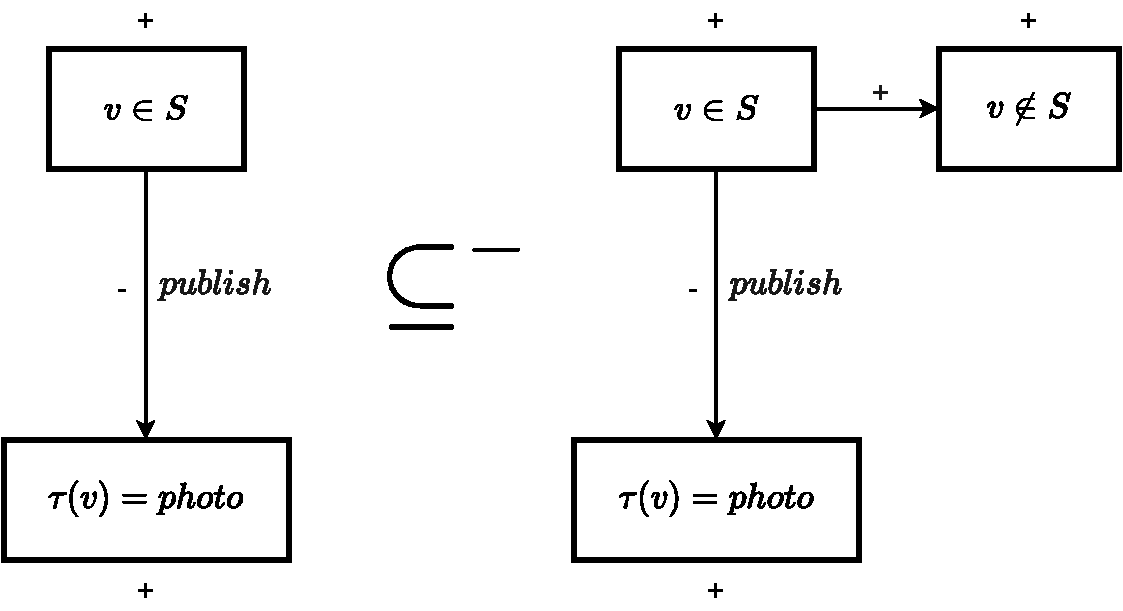
\includegraphics[scale=0.5]{png/FIG2.pdf}
    \end{center}
    \caption{%
        $Q^-$-conservative extension
    }%
    \label{ejemplo-conservativa}
\end{figure}

Since negative nodes introduce non-existence constraints to subgraph verification, $Q^-$-conservative extensions guarantee that no new constraints are added to them. Therefore:

\begin{theorem}{}
    If $Q_2\subseteq^- Q_1$ then $Q_1\preceq Q_2$.
\end{theorem}
\begin{proof}{}
	Since predicates associated to edges are solely based on the information within the edge itself (which takes into account the value of $\theta$ in its incident nodes, irrespective of their $\alpha$ value), we can assert that:
	$$\forall e\in E_{Q_2}\ ({Q_1}_e^{\alpha(e)}={Q_2}_e^{\alpha(e)})$$
	
	Considering this fact, we examine the behaviour of predicates associated with the nodes for both queries:
	\begin{itemize}
		\item If  $n\in V_{Q_2}^-$, since $Q_2\subseteq^- Q_1$, then ${Q_1}_n^-={Q_2}_n^-$.
		\item If $n\in V_{Q_2}^+$, then ${Q_1}_n^+\rightarrow {Q_2}_n^+$, because ($\gamma_1$, $\gamma_2$ are the incidence functions of $Q_1$ and $Q_2$, respectively):
		\begin{align*}
		{Q_1}_n^+   &= \exists v\in V\ \left( \bigwedge_{e\in \gamma_1(n)} {Q_1}_e^{\alpha(e)}\right)\\
		&= \exists v\in V\left( \bigwedge_{e\in \gamma_1(n)\cap E_{Q_2}} {Q_1}_e^{\alpha(e)}\ \wedge \ \bigwedge_{e\in \gamma_1(n)\smallsetminus E_{Q_2}} {Q_1}_e^{\alpha(e)}\right)\\
		&= \exists v\in V\left( \bigwedge_{e\in \gamma_2(n)\cap E_{Q_2}} {Q_2}_e^{\alpha(e)}\ \wedge \ \bigwedge_{e\in \gamma_1(n)\smallsetminus E_{Q_2}} {Q_1}_e^{\alpha(e)}\right)\\
		&\rightarrow {Q_2}_n^+
		\end{align*}
	\end{itemize}
	Hence:
	\begin{align*}
	Q_1 &= \bigwedge_{n\in V_{Q_1}} {Q_1}_n^{\alpha(n)} = \bigwedge_{n\in V_{Q_2}} {Q_1}_n^{\alpha(n)} \ \wedge \ \bigwedge_{n\in V_{Q_1}\smallsetminus V_{Q_2}} {Q_1}_n^{\alpha(n)}\\
	&= \bigwedge_{n\in V_{Q_2}^+} {Q_1}_n^{\alpha(n)} \ \wedge \ \bigwedge_{n\in V_{Q_2}^-} {Q_1}_n^{\alpha(n)} \ \wedge \ \bigwedge_{n\in V_{Q_1}\smallsetminus V_{Q_2}} {Q_1}_n^{\alpha(n)}
	\end{align*}
	\begin{align*}
	&\rightarrow \bigwedge_{n\in V_{Q_2}^+} {Q_2}_n^{\alpha(n)} \ \wedge \ \bigwedge_{n\in V_{Q_2}^-} {Q_2}_n^{\alpha(n)} \ \wedge \ \bigwedge_{n\in V_{Q_1}\smallsetminus V_{Q_2}} {Q_1}_n^{\alpha(n)}\\ 
	&= \bigwedge_{n\in V_{Q_2}} {Q_2}_n^{\alpha(n)} \ \wedge \ \bigwedge_{n\in V_{Q_1}\smallsetminus V_{Q_2}} {Q_1}_n^{\alpha(n)}\\
	&\rightarrow {Q_2}
	\end{align*}
\end{proof}
Previous result suggests that a query can be refined by adding nodes (of any sign) and edges to the existing positive nodes, but because of the (negated) interpretation of predicates associated with negative nodes, care must be taken to maintain their neighborhood to be sure that adding more edges does not weaken the imposed conditions (which consequently will not provide refined predicates).

To achieve controlled methods of query generation, we will outline processes for refining queries through unit steps. We shall accomplish this by defining the cloning operation, whereby existing nodes are duplicated, and all incident edges (including those between the nodes) on the original graph are also cloned: 

\begin{definition}{}
    Given $G=(V,E,\mu)$, and $W\subseteq V$, we define the \emph{clone of $G$ by duplication of $W$}, $Cl_G^W$, as:
    
    $$Cl_G^W=(V\cup W',E\cup E',\mu\cup \{(n',\mu(n))\}_{n\in W}\cup \{(e',\mu(e))\}_{e'\in E'})$$
    where $W'=\{n'\ :\ n\in W\}$ are new cloned nodes from $W$, and $ E '$ is a set of new edges obtained from incident edges on nodes of $ W $ where nodes of $ W $ are replaced by copies of $ W' $ (edges connecting original nodes with cloned nodes and edges connecting cloned nodes, are cloned).
\end{definition}\medskip

Figure \ref{ejemplo-clonacion} shows an example of a cloned graph by duplicating two nodes (in the original graph, left side, the set of nodes to be duplicated is highlighted).
\begin{figure}[h]
    \begin{center}
        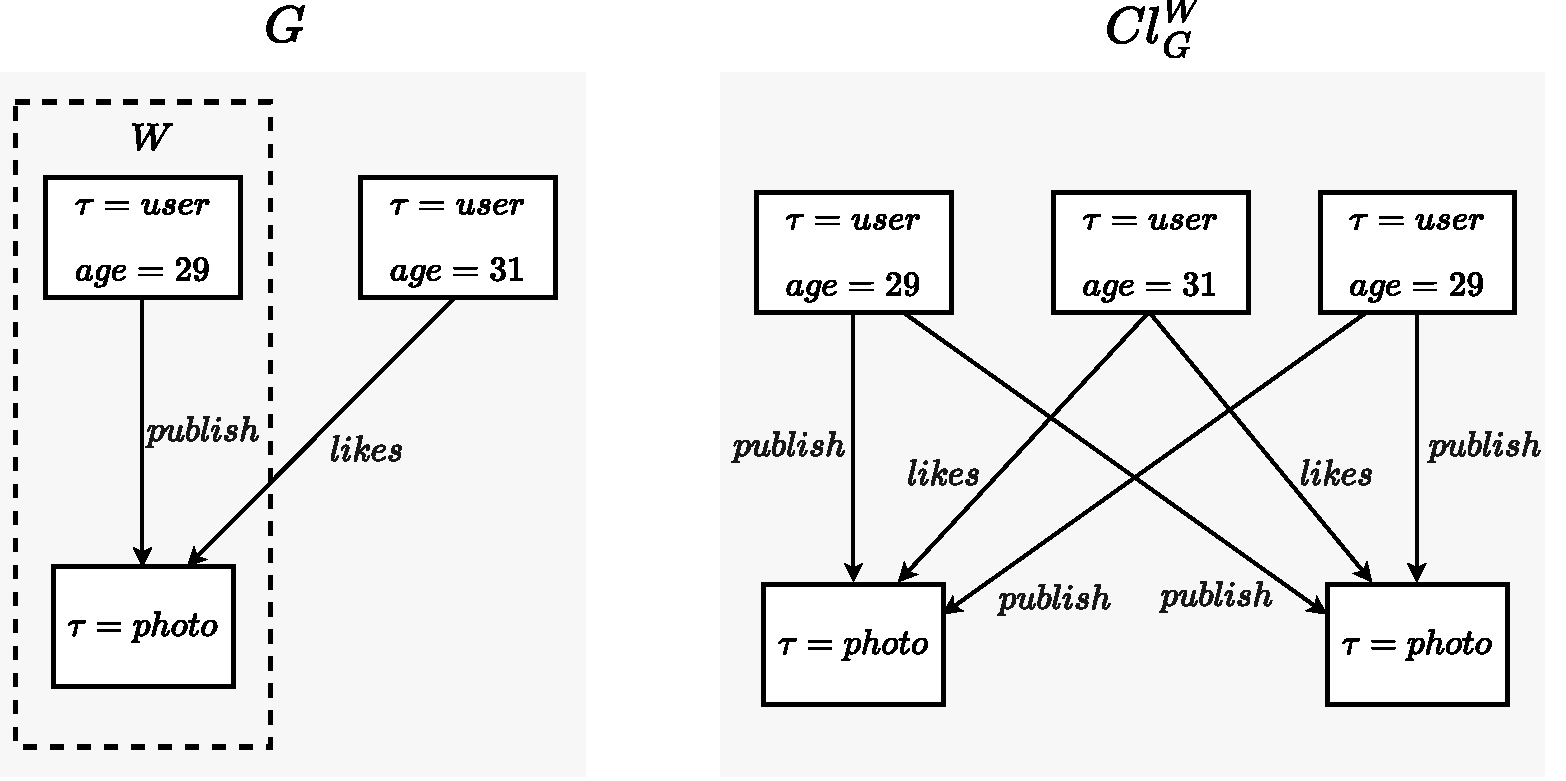
\includegraphics[width=\columnwidth]{png/FIG3.pdf}
    \end{center}
    \caption{%
        Clone of a graph by duplication
    }%
    \label{ejemplo-clonacion}
\end{figure}

The next result indicates that duplicating positive nodes does not change the \textit{meaning} of the queries.

\begin{theorem}{}
    If $W\subseteq V^+_Q$, then $Cl_Q^W\equiv Q$.
\end{theorem}
\begin{proof}{}
	Let us denote $ Q_1 = Cl_Q^W $. Then:
	\begin{align*}
	Q_1 &= \bigwedge_{n\in V_{Q_1}} {Q_1}_n^{\alpha(n)}
	 =\bigwedge_{n\in V_Q} {Q_1}_n^{\alpha(n)}\ \wedge \ \bigwedge_{n\in W} {Q_1}_{n'}^{\alpha(n')}\\
	&= \bigwedge_{n\in V_Q\smallsetminus \gamma_Q(W)} {Q_1}_n^{\alpha(n)}\ \wedge \ \bigwedge_{n\in\gamma_Q(W)} {Q_1}_n^{\alpha(n)}\ \wedge \ \bigwedge_{n\in W} {Q_1}_{n'}^{\alpha(n')}\\
	&= \bigwedge_{n\in V_Q\smallsetminus \gamma_Q(W)} Q_n^{\alpha(n)}\ \wedge \bigwedge_{n\in\gamma_Q(W)} Q_n^{\alpha(n)}\ \wedge \ \bigwedge_{n\in W} Q_n^{\alpha(n)}\\
	&= Q
	\end{align*}
\end{proof}

When refining a query to find complementary sets of selected subgraphs, we define the concept of a refinement set as central:

\begin{definition}{}
    Given $Q\in \mathcal{Q}$, $R\subseteq \mathcal{Q}$ is a \emph{refinement set} of $Q$ in $G$ if:
    \begin{enumerate}
        \item $\forall\ Q'\in R\ (Q'\preceq_G Q).$
        \item $\forall\ S\subseteq G\ (S\vDash Q\Rightarrow \exists !\ Q'\in R\ (S\vDash Q')).$
    \end{enumerate}
\end{definition}\medskip

Let us now introduce refinement sets to enhance simpler queries for expressiveness. $Q\in\mathcal{Q}$ is prefixed, and $\top$ represents a tautology:

\begin{theorem}{(Add new node)}
    If $m\notin V_Q$, the set $Q+\{m\}$, formed by:
        \begin{align*}
        Q_1 &= (V_Q\cup\{m\},\ E_Q,\ \alpha_Q\cup(m,+),\ \theta_Q\cup(m,\top)) , \\ 
         Q_2 &= (V_Q\cup\{m\},\ E_Q,\ \alpha_Q\cup(m,-),\ \theta_Q\cup(m,\top))
        \end{align*}
    is a refinement set of $Q$ in $G$ (Fig. \ref{ref1}).
\end{theorem}
\begin{proof}{}
	We must verify the two necessary conditions for refinement sets:
	\begin{enumerate}
		\item Since $Q\subseteq^- Q_1$ and $Q\subseteq^- Q_2$, thus $Q_1\preceq Q$ and $Q_2\preceq Q$.
		\item Given $S\subseteq G$ such that $S\vDash Q$. Then:
		\begin{align*}
		Q_1&= Q\ \wedge\ Q_m ,\\
		Q_2&= Q\ \wedge\ \neg Q_m 
		\end{align*}
		where $Q_m=\exists v\in V\ (\top)$.
		
		If $G\neq \emptyset$, then $S\vDash Q_1$ and $S\nvDash Q_2$.
		
		If $G= \emptyset$, then $S\nvDash Q_1$ and $S\vDash Q_2$.
	\end{enumerate}
\end{proof}

Since $ G \neq \emptyset $ (usually), $ Q_1 \equiv Q $. However, although we obtain an equivalent query, this operation is beneficial for adding new nodes and restrictions in the future.

\begin{figure}[h]
    \begin{center}
        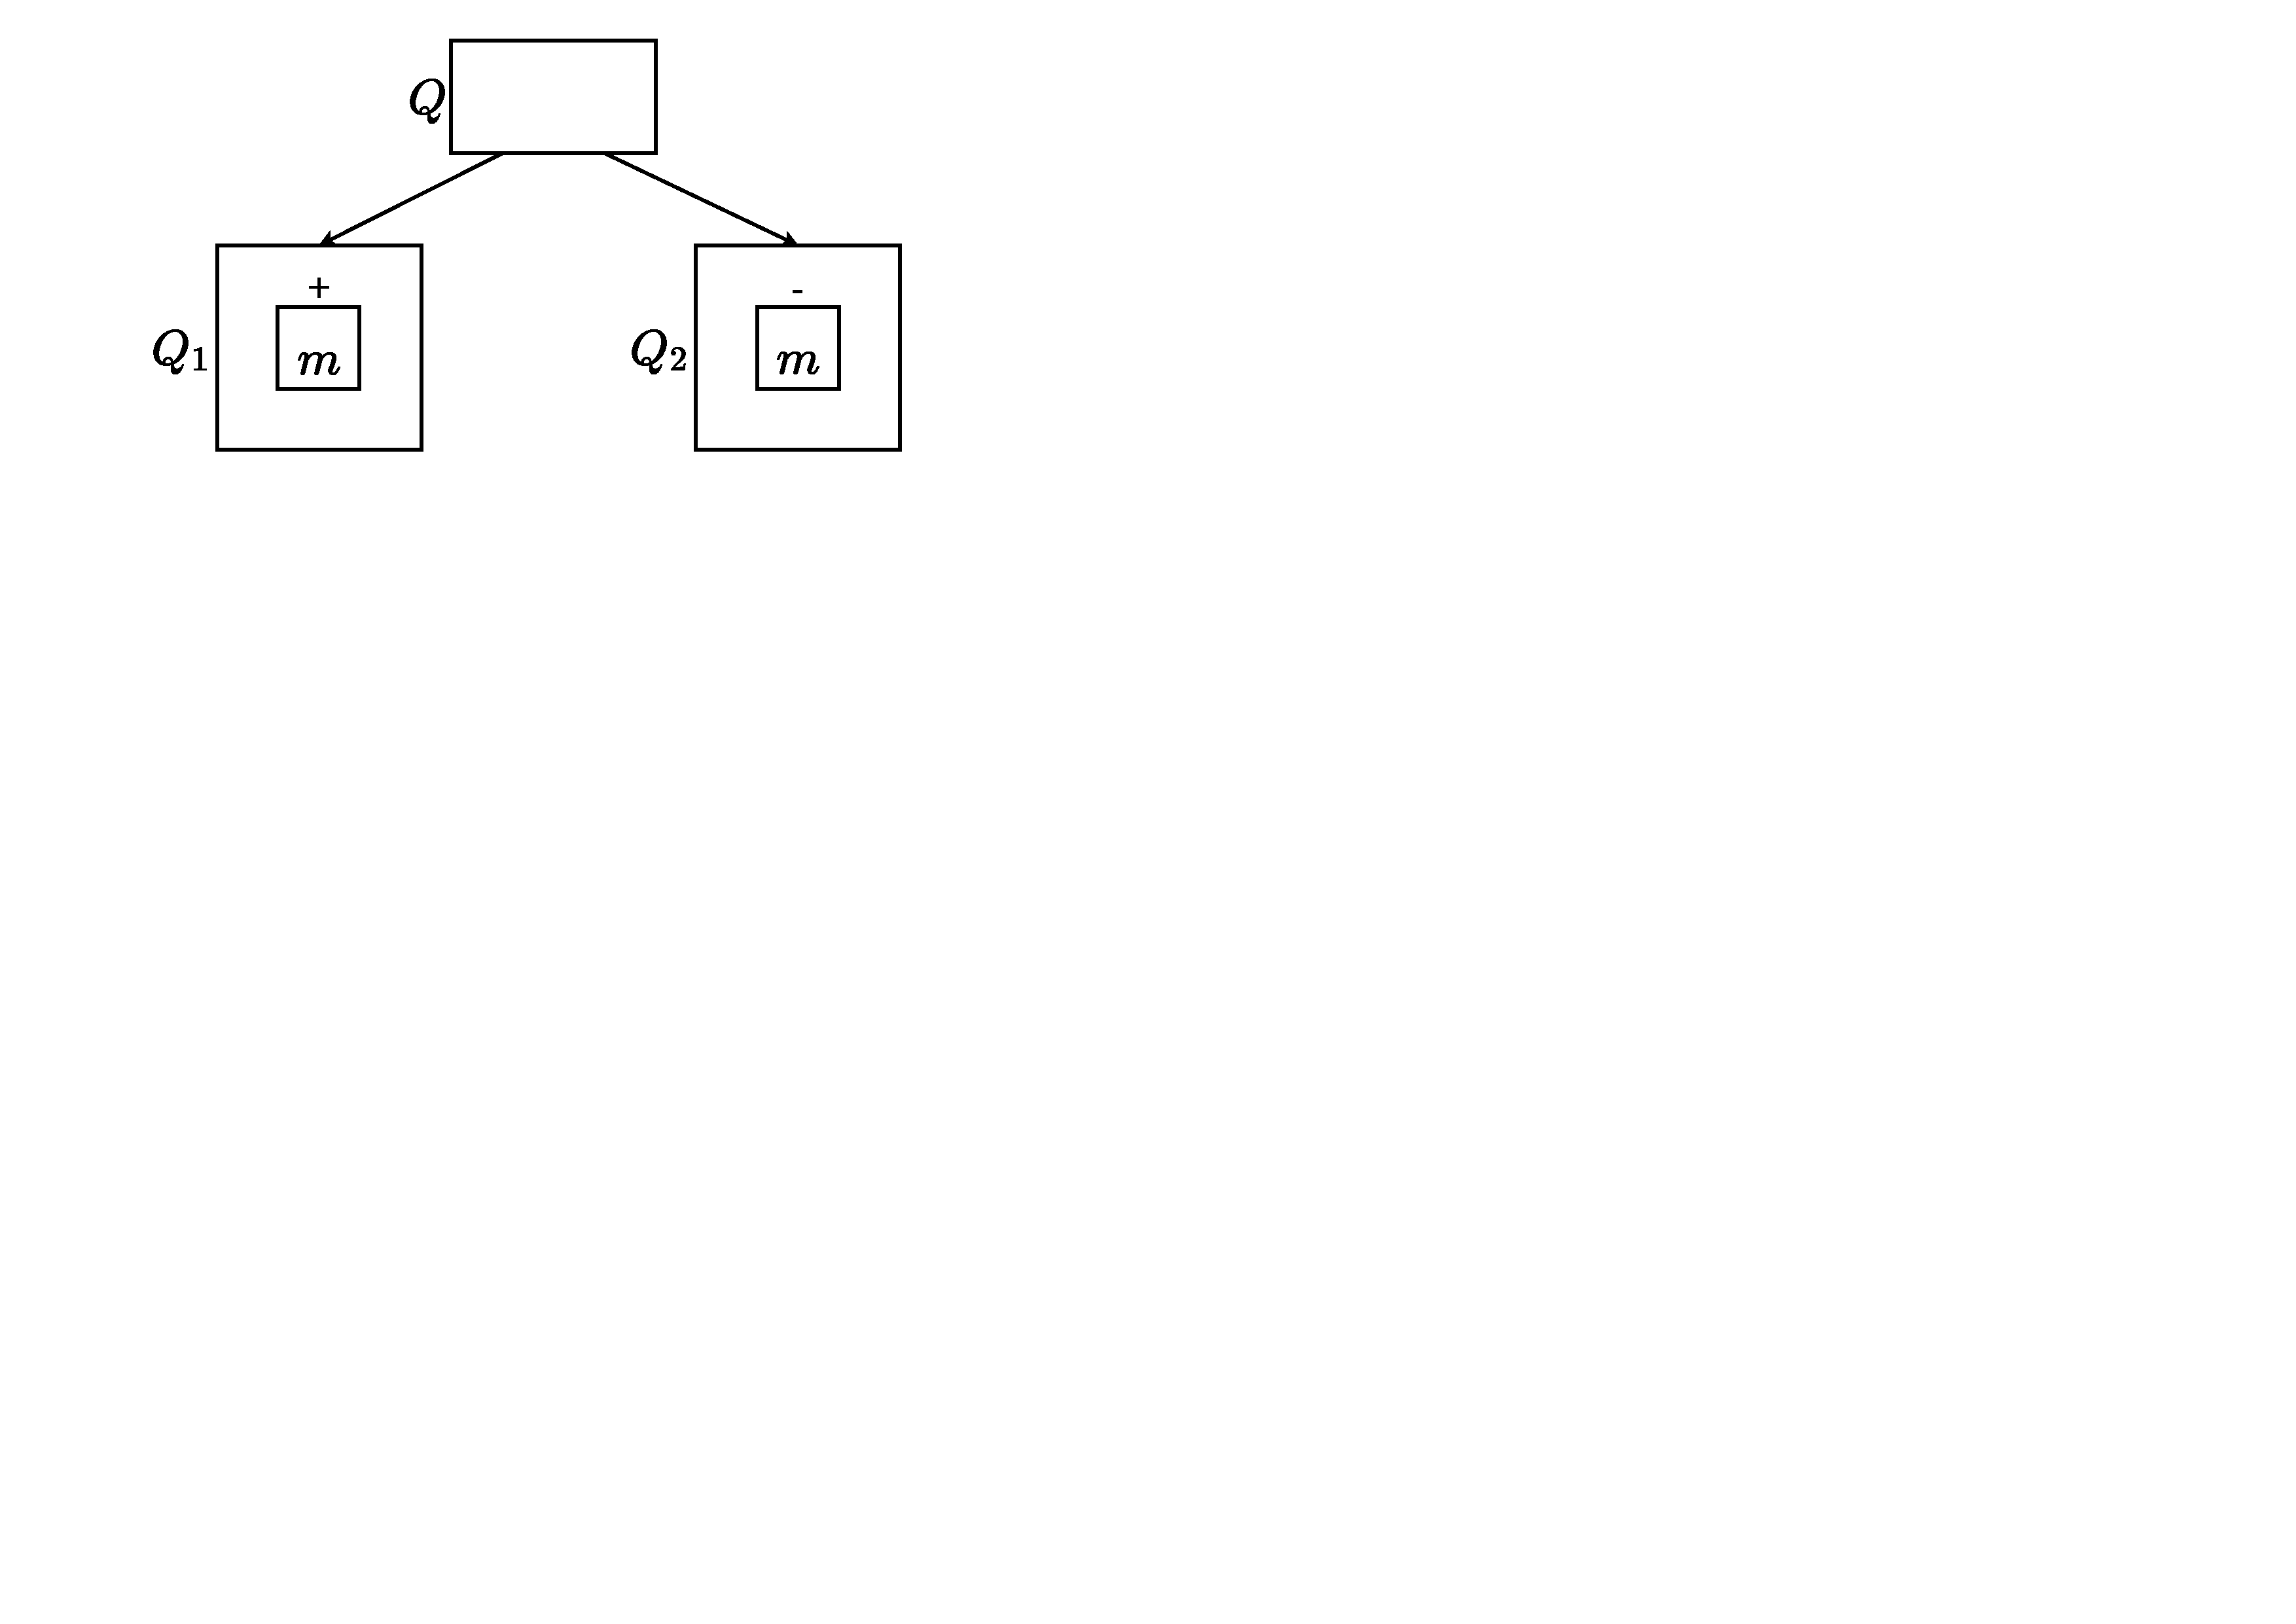
\includegraphics[scale=0.3]{png/REF1.pdf}
    \end{center}
    \caption{%
        \textit{Add node} refinement
    }%
    \label{ref1}
\end{figure}

The second refinement allows for the establishment of edges between query nodes that already exist. To obtain a valid refinement set, the inclusion of edges is limited to positive nodes. Subsequently, the nodes marked with a positive/negative sign represent cloned nodes whose $\alpha$ property has been designated as positive/negative.

\begin{theorem}{(Add new edge between + nodes)}
    If $n,m\in V_Q^+$, the set $Q+\{n\stackrel {e^*}{\longrightarrow} m\}$ ($*\in\{+,-\}$), formed by:
    \begin{align*}
    Q_1 &= (V_{Q'},\ E_{Q'}\cup\{n^+\stackrel {e^*}{\longrightarrow} m^+\},\ \theta_{Q'}\cup(e,\top)), \\
    Q_2 &= (V_{Q'},\ E_{Q'}\cup\{n^+\stackrel {e^*}{\longrightarrow} m^-\},\ \theta_{Q'}\cup(e,\top)), \\
    Q_3 &= (V_{Q'},\ E_{Q'}\cup\{n^-\stackrel {e^*}{\longrightarrow} m^+\},\ \theta_{Q'}\cup(e,\top)), \\
    Q_4 &= (V_{Q'},\ E_{Q'}\cup\{n^-\stackrel {e^*}{\longrightarrow} m^-\},\ \theta_{Q'}\cup(e,\top))
\end{align*}
    (where $Q'=Cl_Q^{\{n,m\}}$) is a refinement set of $Q$ in $G$ (Fig. \ref{ref2}).
\end{theorem}
\begin{proof}{}
	\quad
	\begin{enumerate}
		\item Since $Q'$ is a clone of $Q$, then $Q\equiv Q'$. In addition,  $Q'\subseteq^- Q_1,Q_2,Q_3,Q_4$, thus $Q_1,Q_2,Q_3,Q_4\preceq Q'\equiv Q$.
		\item Let us consider the predicates:
		\begin{align*}
		P_n &= \exists v\in V\ \left( \bigwedge_{a\in \gamma(n)} Q_a^{\alpha(a)}\ \wedge Q_{e^o}^{\alpha(e)}\right), \\
		P_m &= \exists v\in V\ \left( \bigwedge_{a\in \gamma(m)} Q_a^{\alpha(a)}\ \wedge Q_{e^i}^{\alpha(e)}\right).
		\end{align*}
		If $S\vDash Q_n$ and $S\vDash Q_m$, then we have four mutually complementary options:
		\begin{itemize}
			\item $S\vDash P_n\ \wedge\ S\vDash P_m \Rightarrow S\vDash Q_1$
			\item $S\vDash P_n\ \wedge\ S\nvDash P_m \Rightarrow S\vDash Q_2$
			\item $S\nvDash P_n\ \wedge\ S\vDash P_m \Rightarrow S\vDash Q_3$
			\item $S\nvDash P_n\ \wedge\ S\nvDash P_m \Rightarrow S\vDash Q_4$
		\end{itemize}
	\end{enumerate}
\end{proof}

\begin{figure}[h]
    \begin{center}
        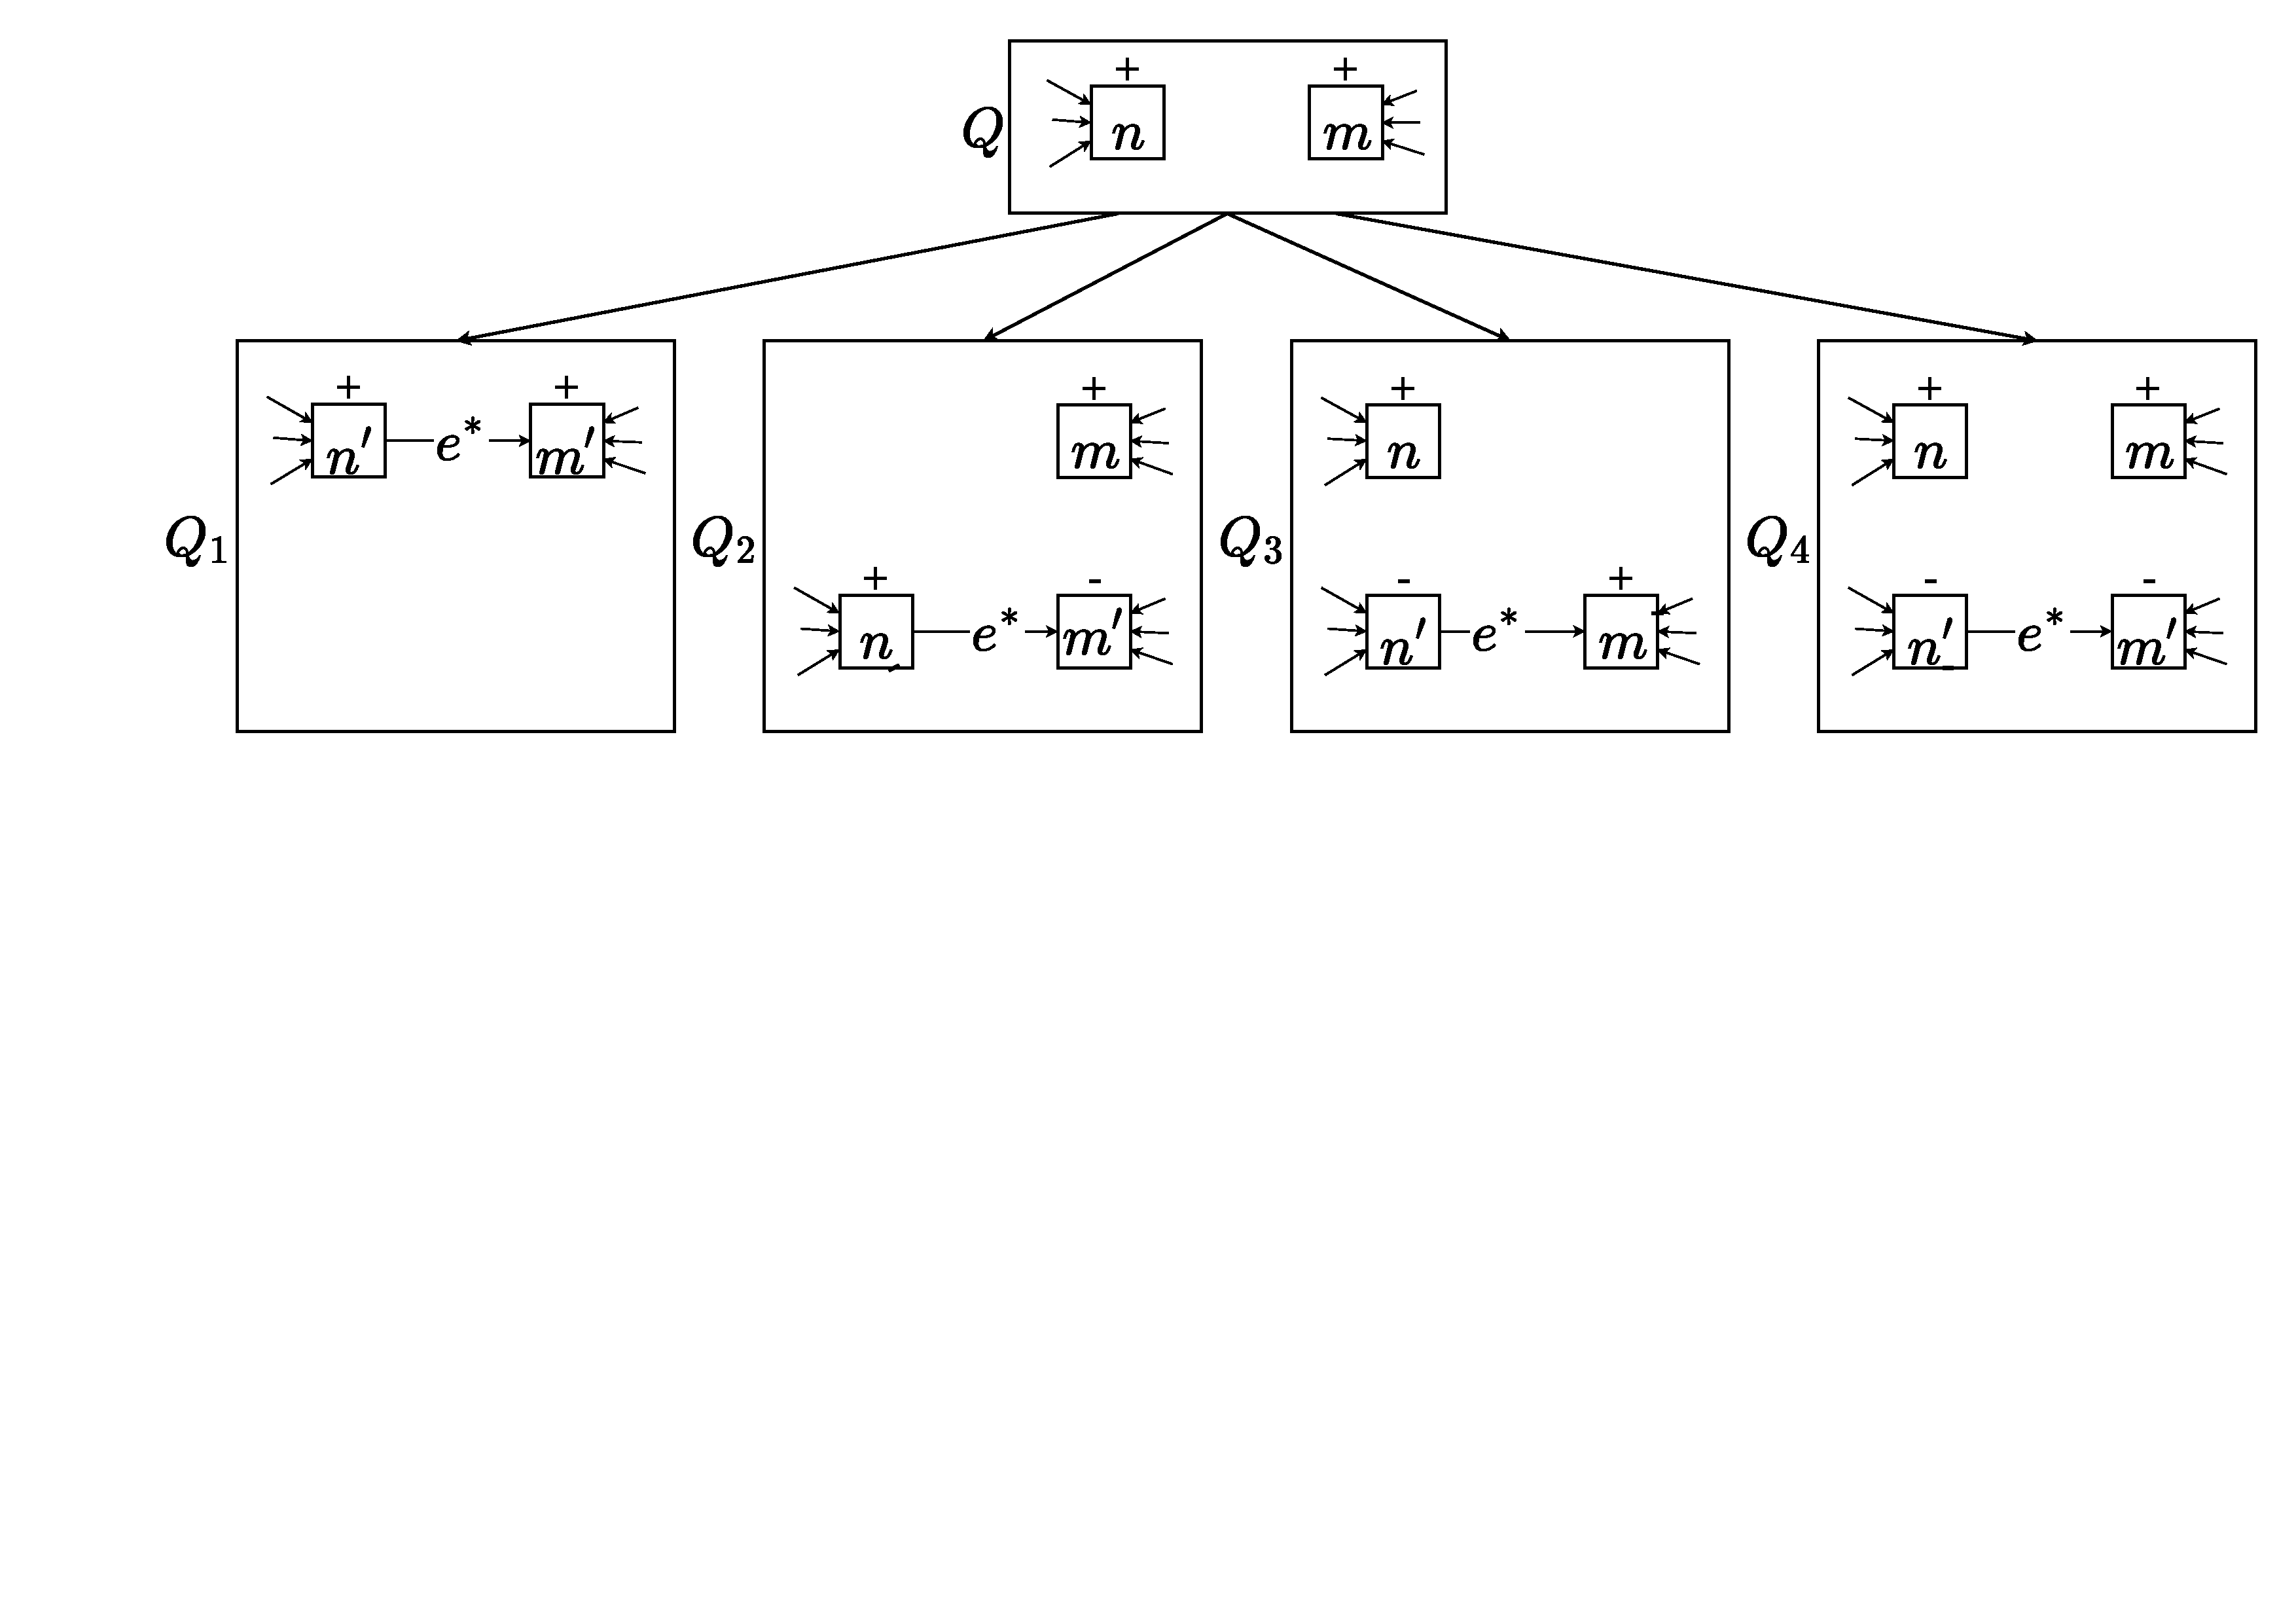
\includegraphics[width=\columnwidth]{png/REF2SIM.pdf}
    \end{center}
    \caption{%
        \textit{Add edge} refinement (simplified)
    }%
    \label{ref2}
\end{figure}

Next, an additional predicate is added to an existing edge through the following operation, limited to positive edges connecting positive nodes.

\begin{theorem}{(Add predicate to + edge between + nodes)}
    If $n,m\in V_Q^+$, with $n\stackrel {e^+}{\longrightarrow} m$, and $\varphi\in Form^2(L)$, the set $Q+\{n\stackrel {e \wedge \varphi}{\longrightarrow} m\}$, formed by:
    \begin{align*}
    Q_1 &= (V_{Q'},\ E_{Q'}\cup\{n^+\stackrel {e'}{\longrightarrow} m^+\},\ \theta_{Q'}\cup(e',\theta_e\wedge \varphi)), \\
    Q_2 &= (V_{Q'},\ E_{Q'}\cup\{n^+\stackrel {e'}{\longrightarrow} m^-\},\ \theta_{Q'}\cup(e',\theta_e\wedge \varphi)), \\
    Q_3 &= (V_{Q'},\ E_{Q'}\cup\{n^-\stackrel {e'}{\longrightarrow} m^+\},\ \theta_{Q'}\cup(e',\theta_e\wedge \varphi)), \\
    Q_4 &= (V_{Q'},\ E_{Q'}\cup\{n^-\stackrel {e'}{\longrightarrow} m^-\},\ \theta_{Q'}\cup(e',\theta_e\wedge \varphi))
    \end{align*}
    (where $Q'=Cl_Q^{\{n,m\}}$) is a refinement set of $Q$ in $G$ (Fig. \ref{ref3}).
\end{theorem}
\begin{proof}{}
	The proof is similar to the previous ones.
\end{proof}

\begin{figure}[h]
    \begin{center}
        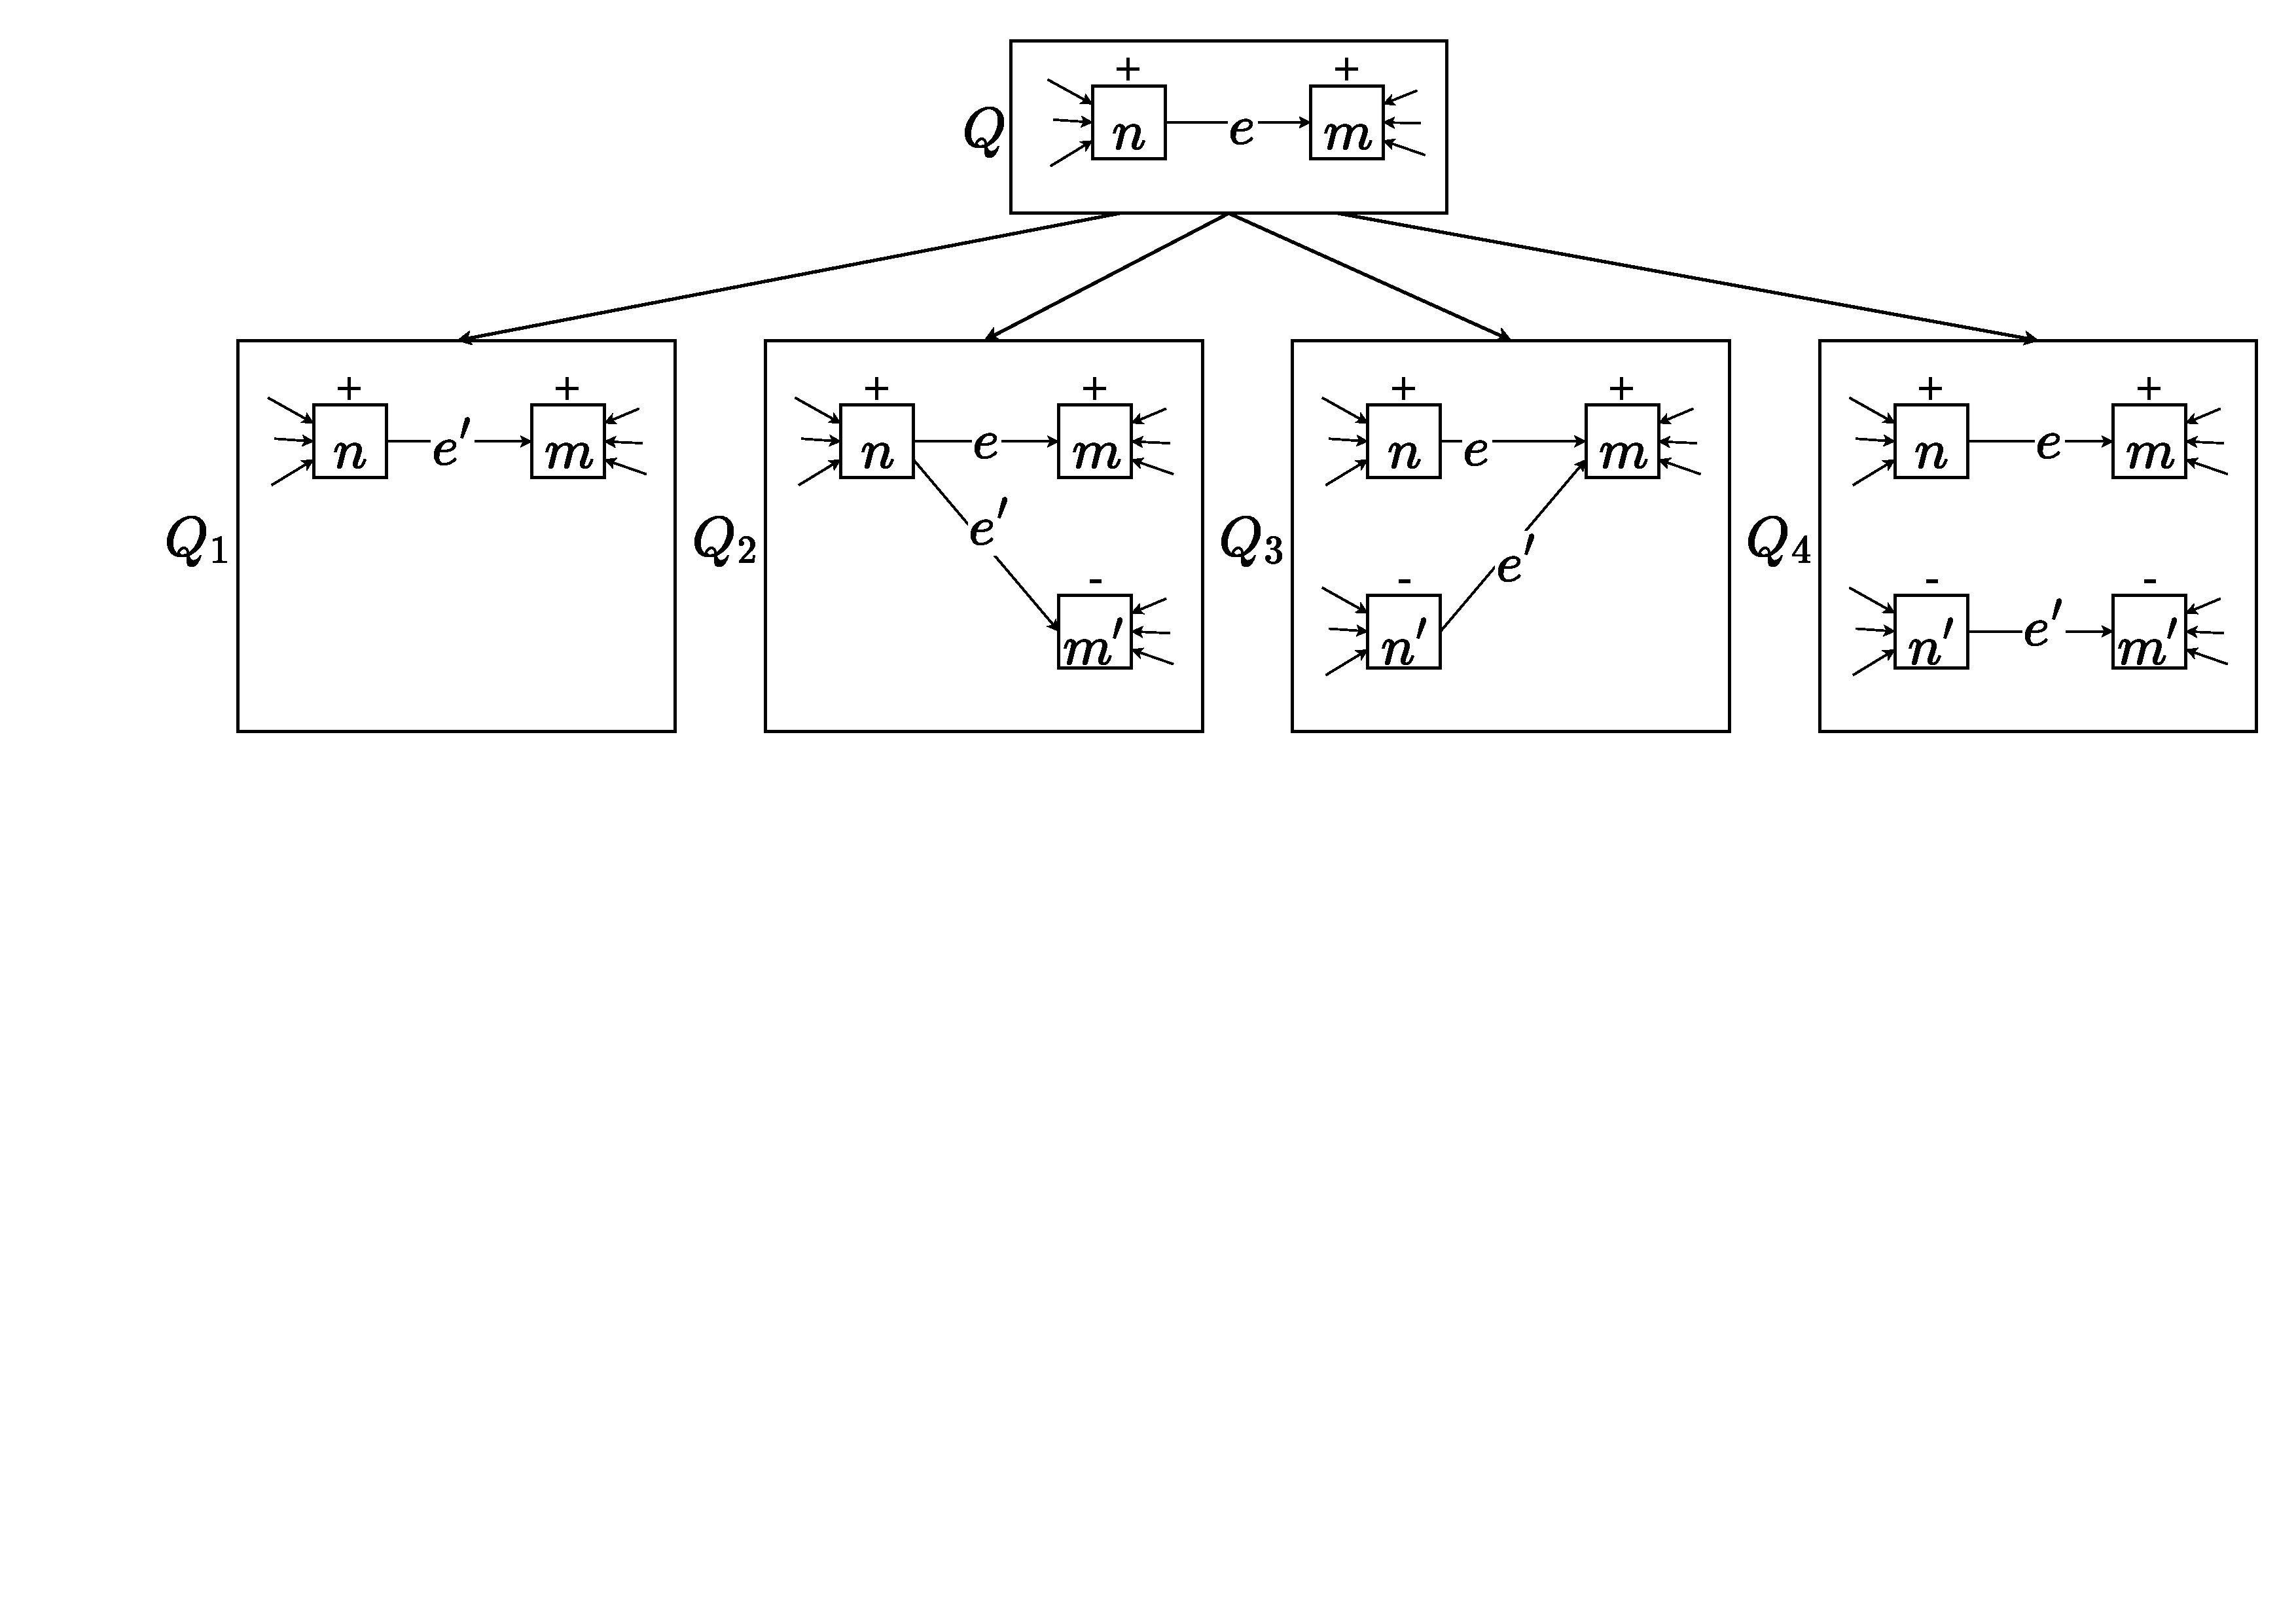
\includegraphics[width=\columnwidth]{png/REF3SIM.pdf}
    \end{center}
    \caption{%
	\textit{Add predicate to edge} refinement (simplified)
    }%
    \label{ref3}
\end{figure}

Finally, the last step involves adding predicates to existing nodes. This operation is only permitted when the affected nodes are positive, including the node where the predicate is added and those connected to it.

\begin{theorem}{(Add predicate to + node with + neighborhood)}
    If $\varphi\in Form^2(L)$, and $n\in V_Q^+$ with $\mathcal{N}_Q(n)\subseteq V_Q^+$, then the set $Q+\{n\wedge \varphi\}$ formed by:
    $$\{Q_{\sigma}=(V_{Q'},E_{Q'},\alpha_{Q'}\cup \sigma,\theta_{Q'}\cup(n',\theta_n\wedge\varphi))\ :\ \sigma\in \{+,-\}^{\mathcal{N}_Q(n)}\}$$ 	
(where $Q'=Cl_Q^{\mathcal{N}_Q(n)}$, and $\{+,-\}^{\mathcal{N}_Q(n)}$ is the set of all possible assignments of signs to elements in $\mathcal{N}_Q(n)$)
is a refinement set of $Q$ in $G$ (Fig. \ref{ref4}).
\end{theorem}
\normalsize
\begin{proof}{}
	The proof resembles earlier ones. It is important to consider that modifying node $n$ not only alters the associated predicate, but also those of its neighboring nodes. Additionally, the set of functions $\{+, -\}^{\mathcal{N}_Q(n)}$ encompasses all feasible sign assignments for the nodes within the neighborhood.
\end{proof}

\begin{figure}[h]
    \begin{center}
        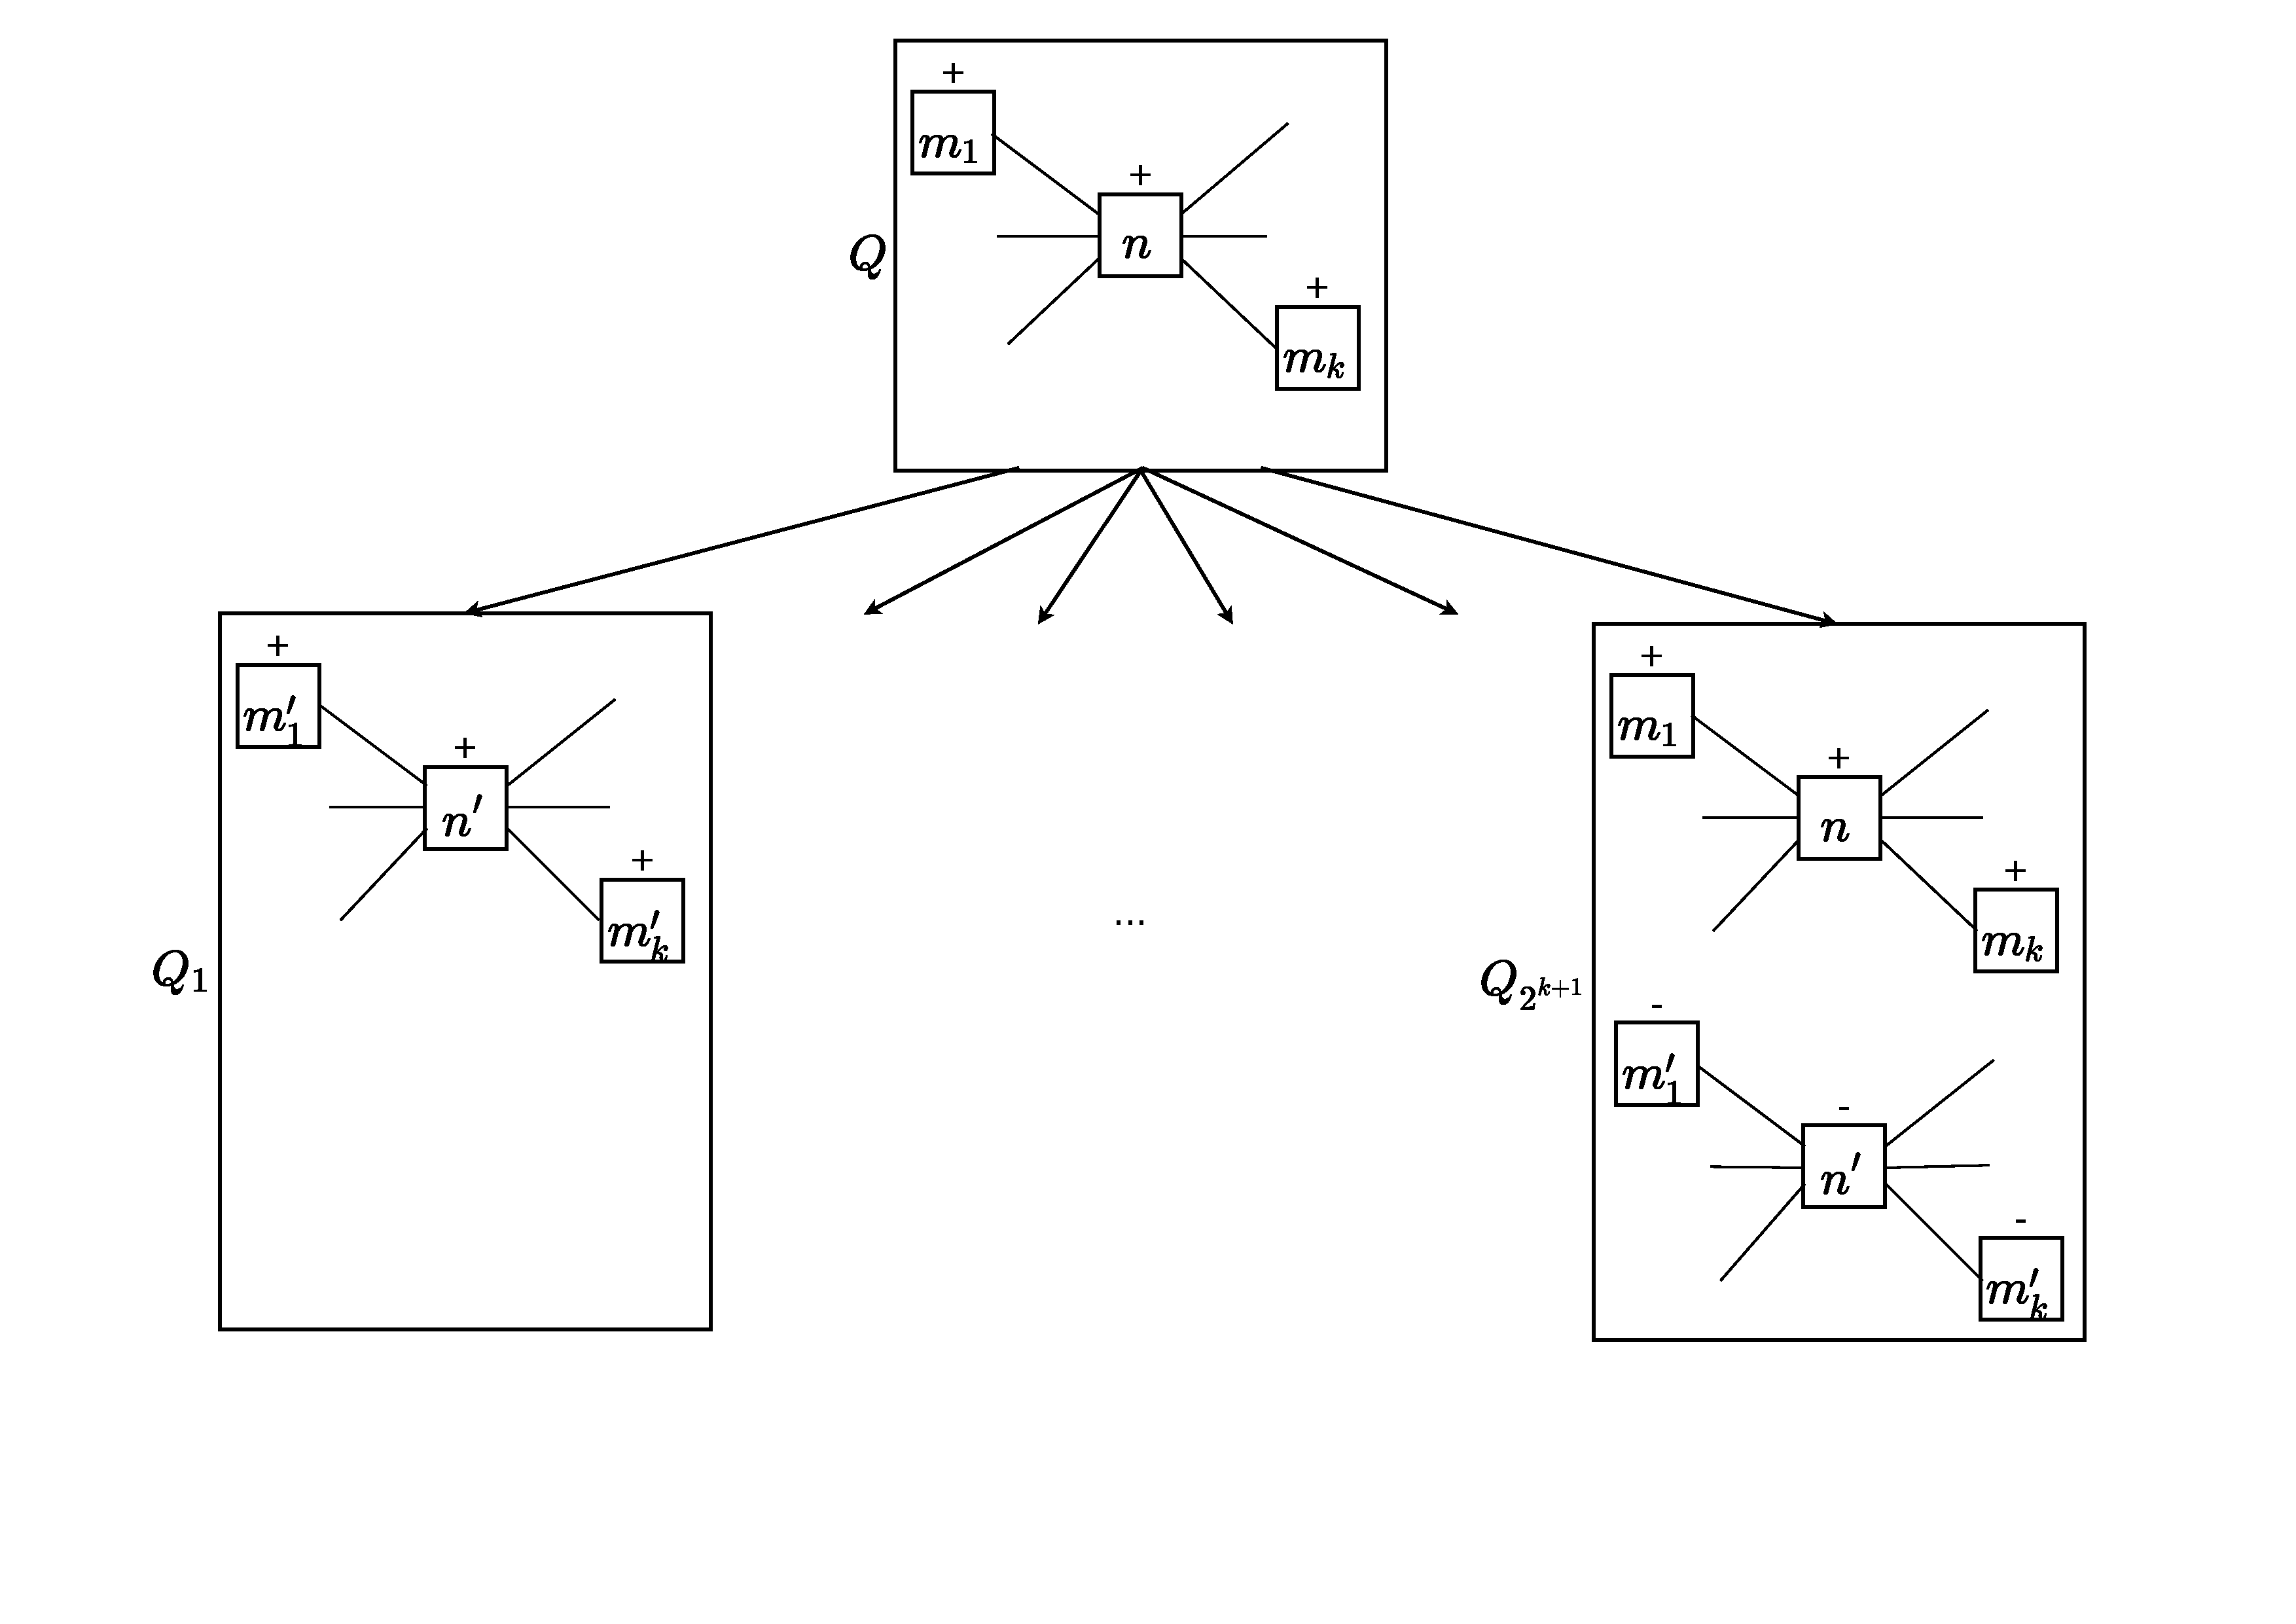
\includegraphics[width=\columnwidth]{png/REF4SIM.pdf}
    \end{center}
    \caption{%
        \textit{Add predicate to node} refinement (simplified)
    }%
    \label{ref4}
\end{figure}

Also note that simplified versions of the refinement sets are shown in Figures \ref{ref1}-\ref{ref4}. Section \ref{simrefs} provides an explanation on how to obtain these simplifications.

Obtaining a complementary query from the structure is a challenging task. Nonetheless, graph analyses often require sequences of queries to verify properties related to refinement and complementarity. To bridge this gap, this section introduces refinement operations. These operations facilitate the construction of an embedded partition tree, where nodes are labelled as illustrated in Figure \ref{arbolGGQ}:

\begin{itemize}
    \item The root node is labeled with $ Q_0 $ (some initial query).
    \item If a node on the tree is labelled with $Q$, and $R=\{Q_1,\dots,Q_n\}$ is a set that refines $Q$, then the child nodes will be labelled with the elements of $R$.
\end{itemize}

\begin{figure}[h]
    \begin{center}
        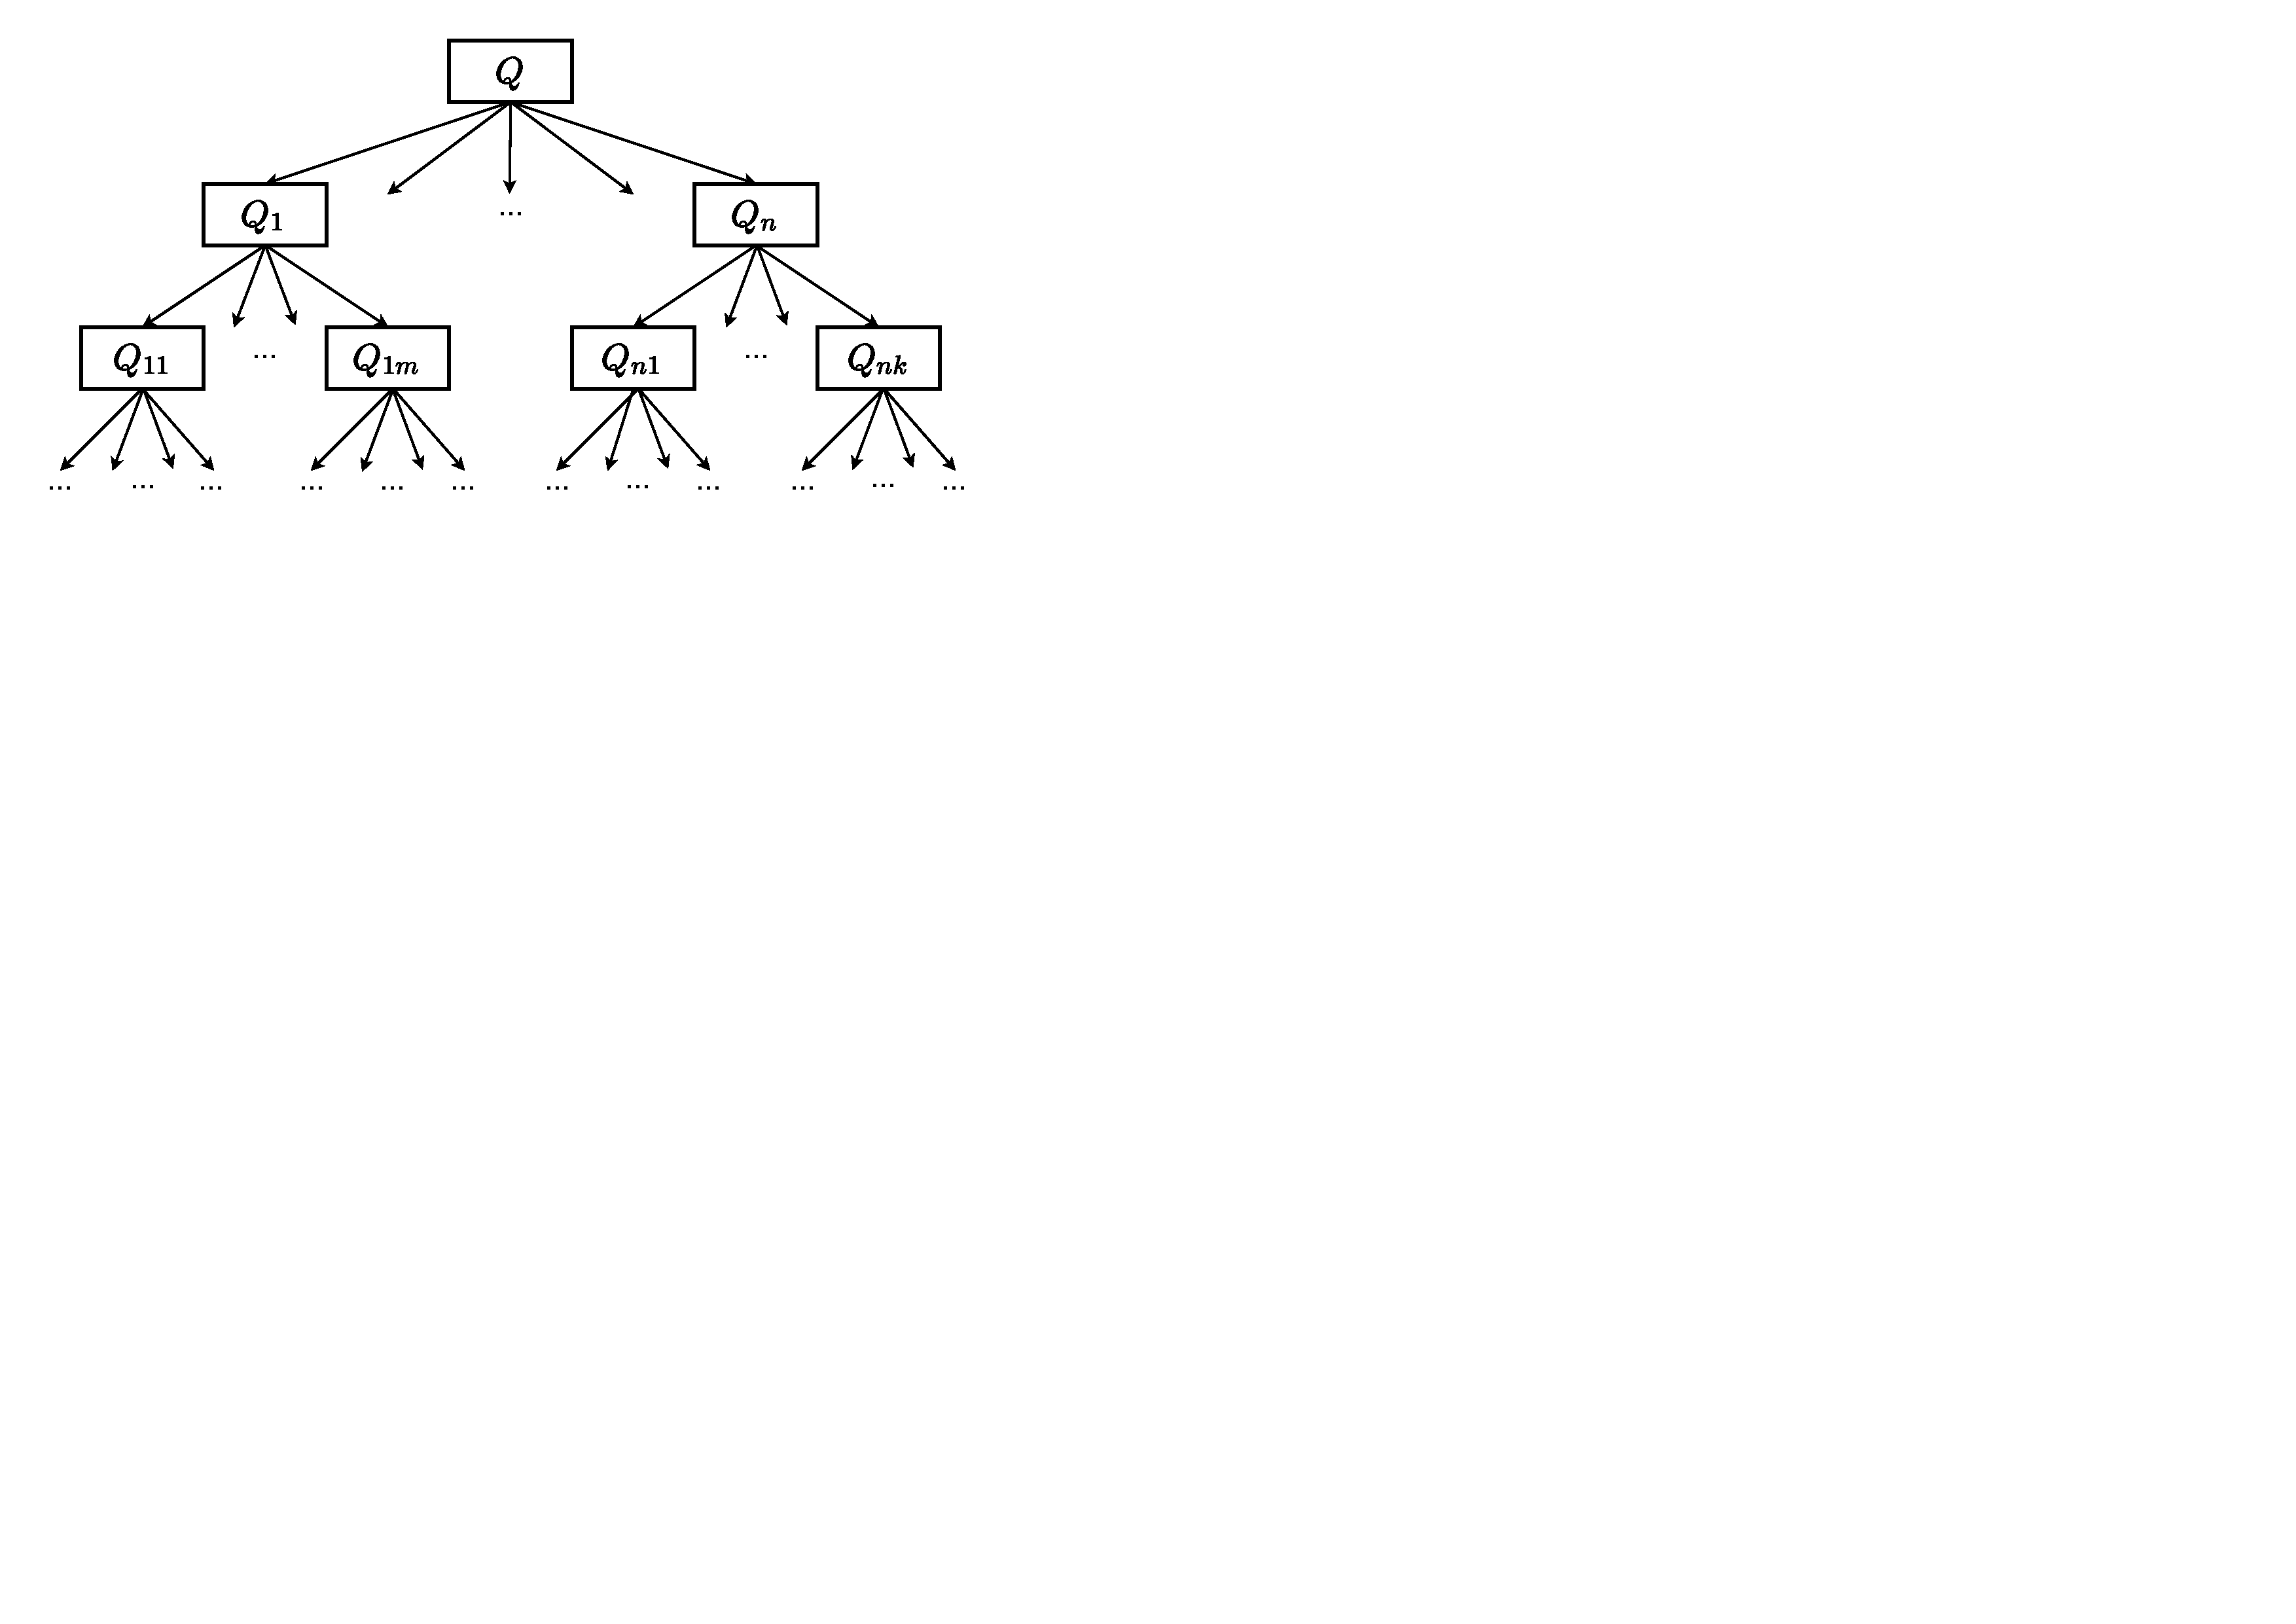
\includegraphics[scale=0.3]{png/FIG4.pdf}
    \end{center}
    \caption{%
        Refinements tree
    }%
    \label{arbolGGQ}
\end{figure}

Refinement sets presented herein offer one approach, rather than the sole approach. For example, we could consider refinements that, instead of adding constraints to positive elements, lighten the conditions over negative elements, for example, by using disjunction of predicates instead of conjunction of them.

\subsection{Simplified refinement sets}
\label{simrefs}
Let us simplify a query into an equivalent one by applying certain operations.

\begin{definition}{}
    We define $Q'\subseteq Q$ as \emph{redundant} in $Q$ if $Q\equiv Q-Q'$. Here, $Q-Q'$ represents the subgraph of $Q$ given by:
	$$(V_Q\smallsetminus V_{Q'}, E_Q\smallsetminus (E_{Q'}\cup\{\gamma(n):\ n\in V_{Q'}\}),\mu_Q)$$

\end{definition}\medskip

One initial finding that enables the acquisition of simplified versions of a query by eliminating superfluous nodes is (from the following two results we only give an idea of the proof, which can be very laborious but straightforward from the above constructions):

\begin{theorem}{}
	Given a query $Q$, and $n,m\in V_Q$ verifying:
	\begin{itemize}
		\item $\alpha(n)=\alpha(m)$
		\item $\theta_n\equiv\theta_m$
		\item For each $e\in \gamma(n)$, exists $e'\in \gamma(m)$, with $\alpha(e)=\alpha(e')$, $\theta_e\equiv\theta_{e'}$ and $\gamma(e)\smallsetminus\{n\}=\gamma(e')\smallsetminus\{m\}$
	\end{itemize}
	Then, $n$ is redundant in $Q$.
\end{theorem}


\begin{proof}{}

A query Q comprises nodes and their relationships. Each query node imposes constraints on the subgraph that is evaluated, including the presence or absence of nodes and the paths in which they participate. These restrictions should be considered during the evaluation. If there are two nodes $n,m \in V_Q$ with $\alpha(n) = \alpha(m)$ and $\theta_n\equiv\theta_m$, and for each $e\in \gamma(n)$, there exists $e'\in \gamma(m)$, with $\alpha(e)=\alpha(e')$, $\theta_e\equiv\theta_{e'}$ and $\gamma(e)\smallsetminus\{n\}=\gamma(e')\smallsetminus\{m\}$, both nodes apply identical restrictions to the subgraph being evaluated. Therefore, deleting one of them will not change the assessment on the subgraph.
\end{proof}


Essentially, $m$ is a duplicate of $n$, but potentially with additional connected edges. A comparable outcome for the edges can be achieved:

\begin{theorem}{}
    Given a query $Q$, and two edges, $e, e'\in E_Q$, such that $\alpha(e)=\alpha(e')$, $n\stackrel {e}{\longrightarrow} m$ and $n\stackrel {e'}{\longrightarrow} m$ with $n,m \in V_Q^+$. If $\theta_e\rightarrow \theta_{e'}$ then $e'$ is redundant in $Q$.
\end{theorem}


\begin{proof}{}

Following the same reasoning as the previous theorem, if there are two edges, $e$ and $e'$, in $E_Q$, which connect the same two nodes in a query and $\alpha(e)=\alpha(e')$ and $\theta_e\rightarrow \theta_{e'}$, the constraint imposed by $e$ implies the constraint imposed by $e'$. Therefore, eliminating e' would maintain the set of matching subgraphs.

\end{proof}

From these two findings, we can streamline the refinement sets that were established in section \ref{refs} by removing redundant elements in succession after cloning. 

\subsection{Graph query examples}

For illustrative purposes, this section presents a series of queries on a toy graph dataset. Figure \ref{starwars} illustrates a segment of the Starwars graph\footnote{http://console.neo4j.org/?id=StarWars}.

\begin{figure}[h!]
    \begin{center}
        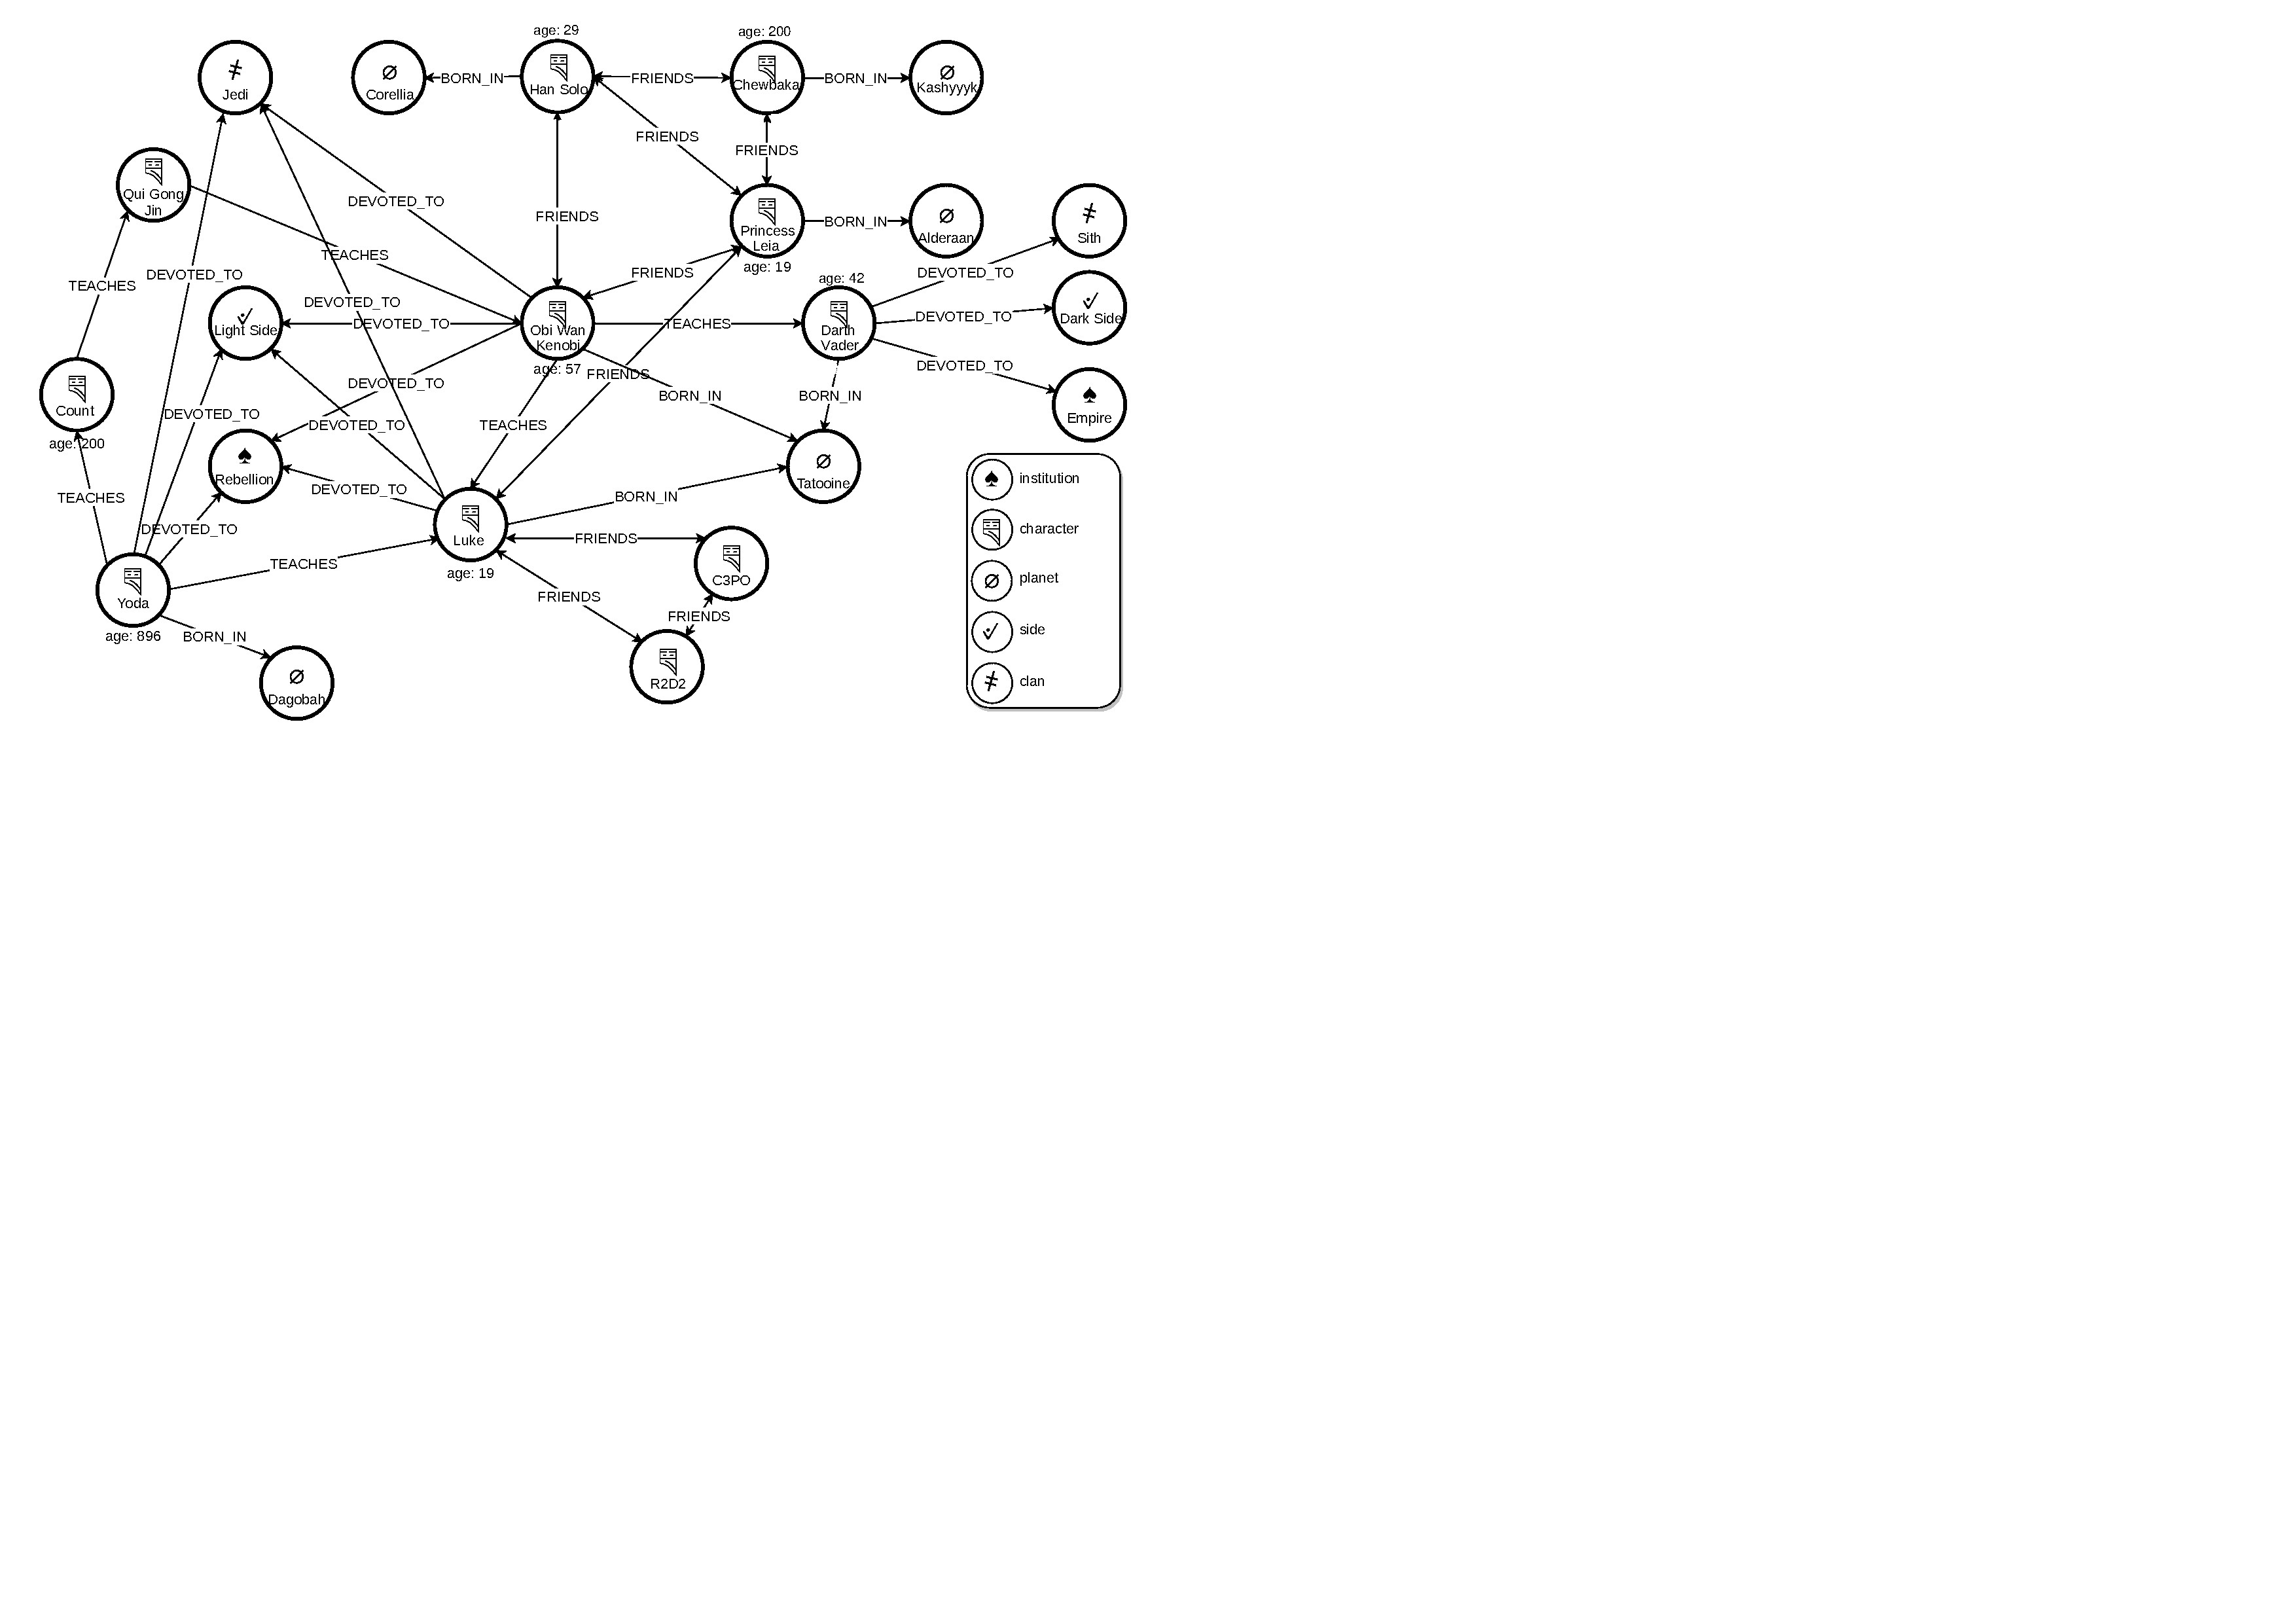
\includegraphics[width=\columnwidth]{png/FIG5.pdf}
    \end{center}
    \caption{%
        Section of Starwars Graph
    }%
    \label{starwars}
\end{figure}

To streamline query and graph representation, we will convert $\tau$, a property denoting node and edge types, into labels for edges or icons for nodes. Additionally, the node properties denoted by \textit{name} will be written on them, and the undirected edges will be represented by bidirectional arrows. The property $\alpha$ will be represented directly on query elements using $+ / -$ symbols, and we will write the binary predicate $\theta$ directly on the elements (except for tautologies). When expressions such as $\tau (\rho) = X$ are in the predicate of an edge, $X$ is written directly and interpreted as a regular expression to be verified by the sequence of $\tau$ properties of the links in the associated graph path. 

\begin{figure}[h!]
    \begin{center}
        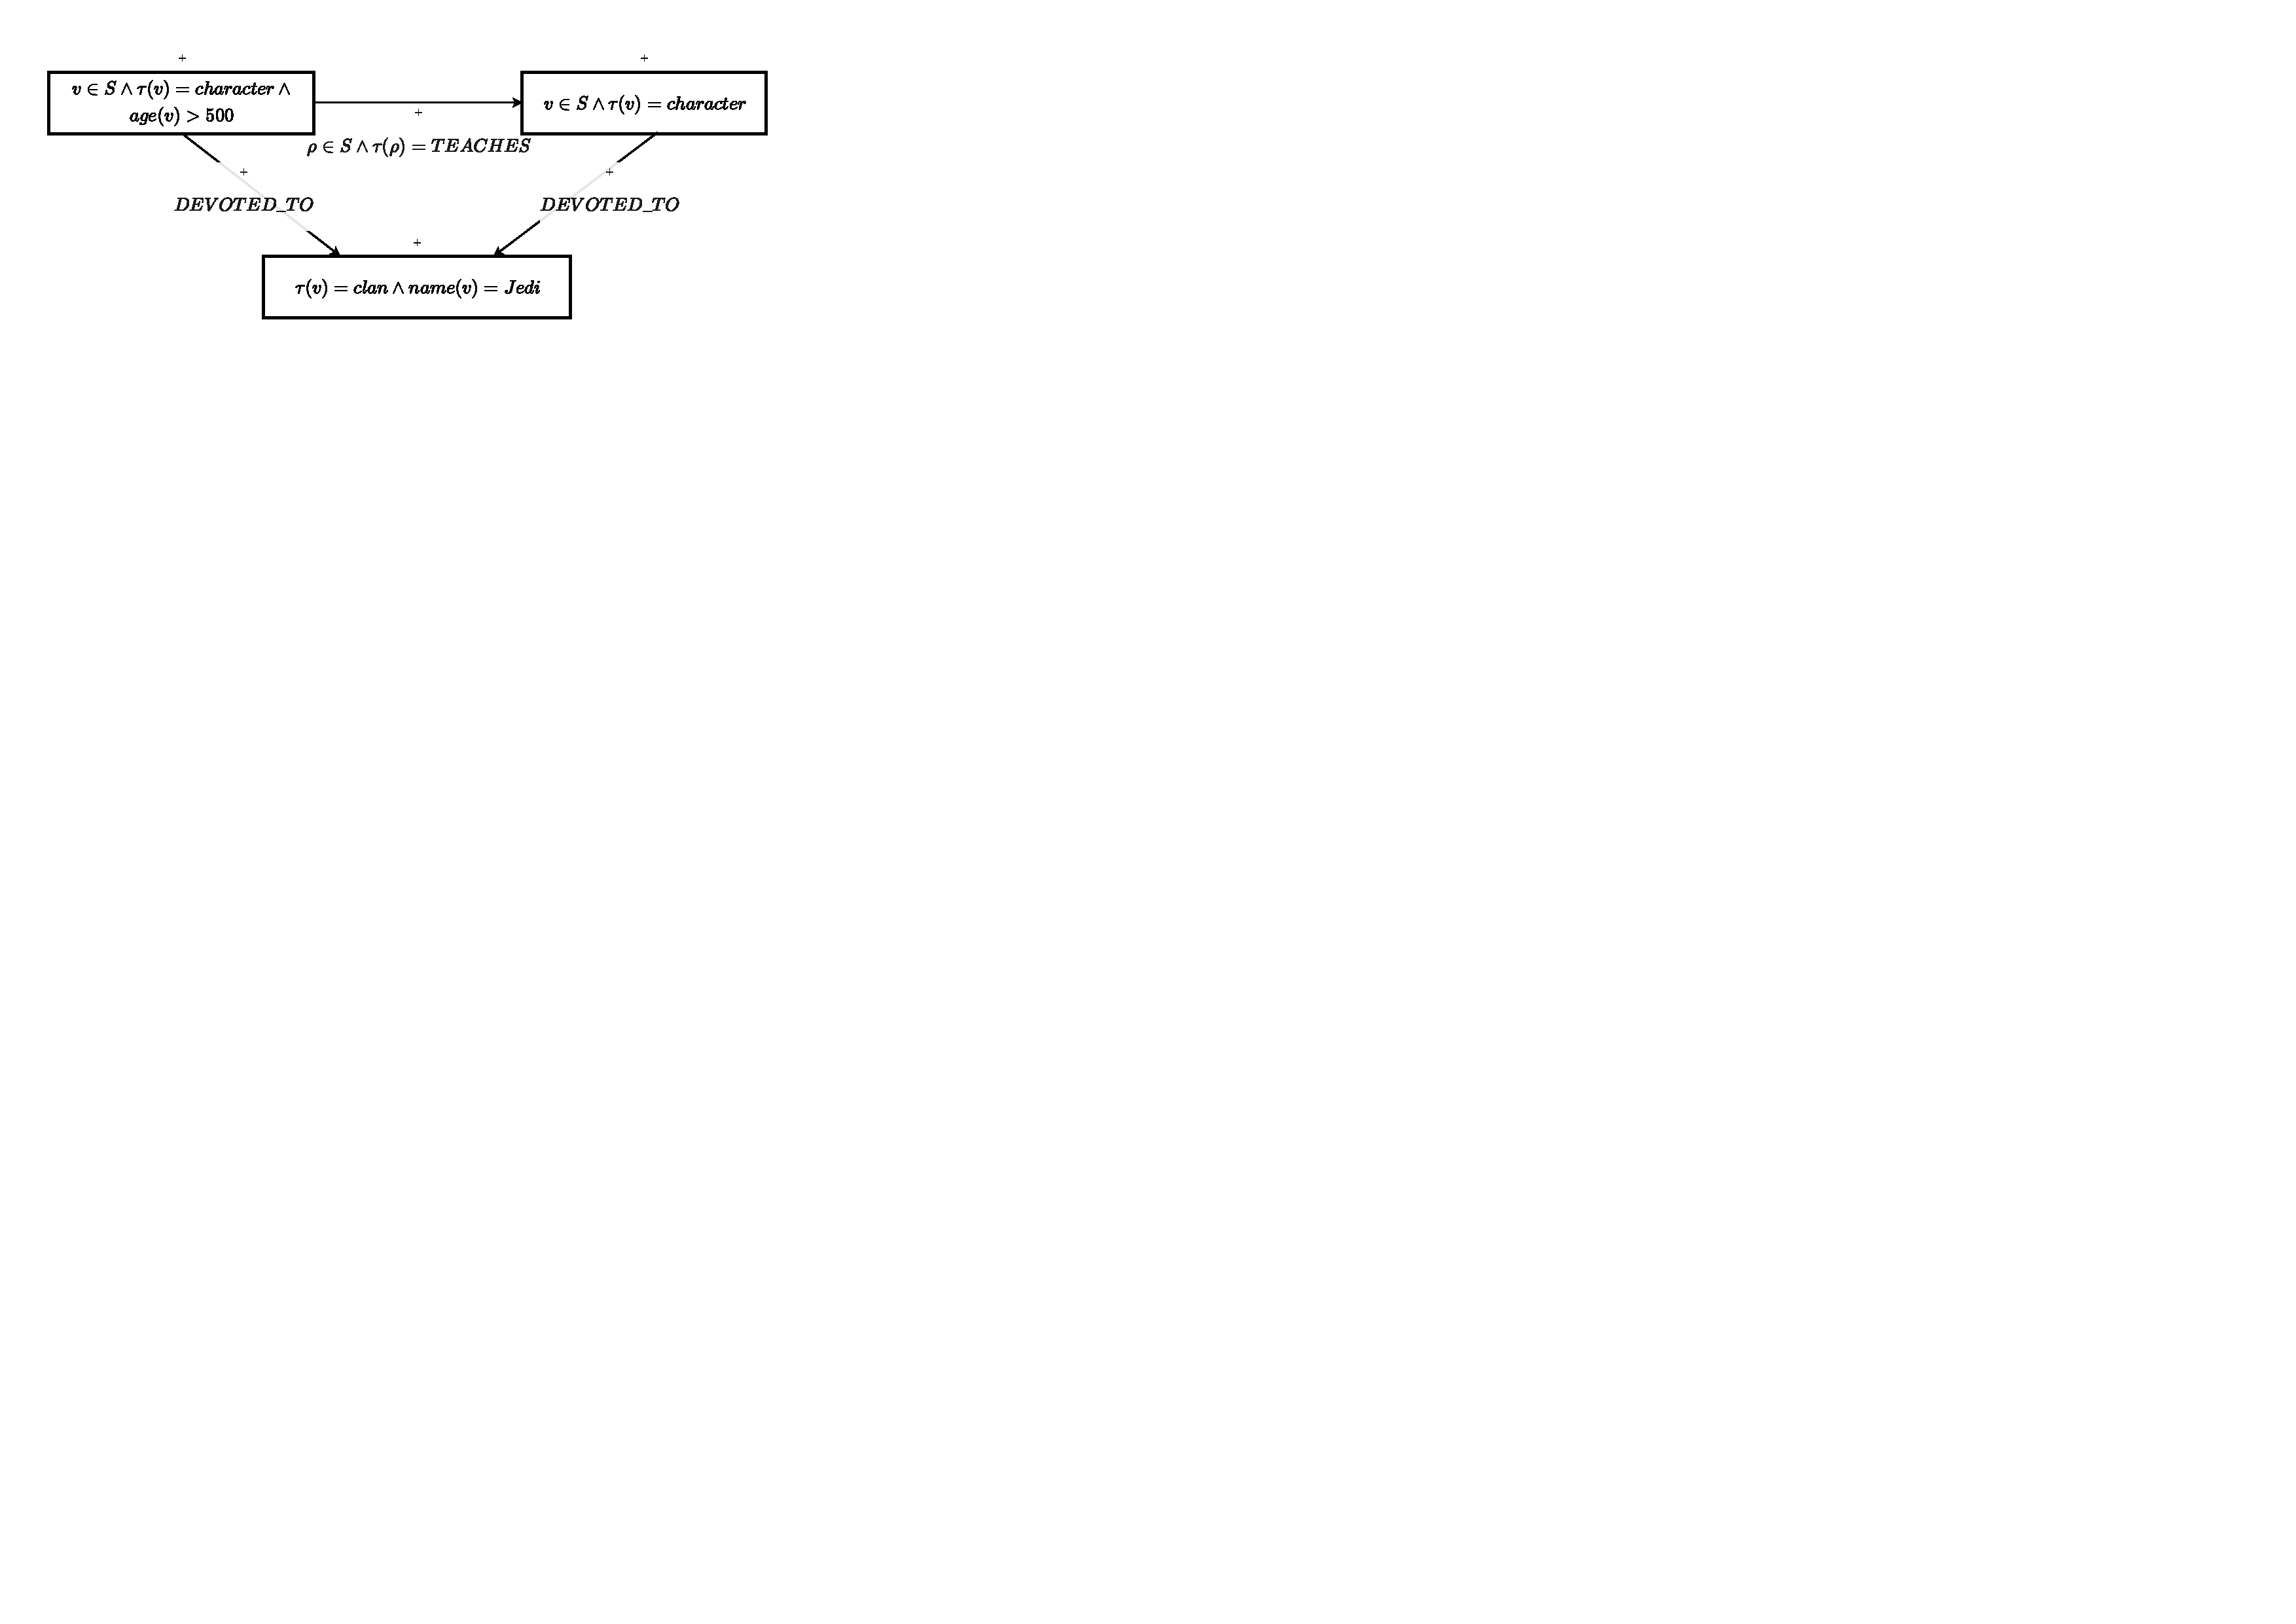
\includegraphics[width=\columnwidth]{png/PQG1.pdf}
    \end{center}
    \caption{%
        Query 1
    }%
    \label{pqg1}
\end{figure}

Query 1 (Figure \ref{pqg1}) can be interpreted as follows: \textit{Two characters are connected by a \textit{TEACHES} relationship, where the master is over 500 years old and both are devoted to the Jedi.} This query utilizes structural constraints through the presence of edges and predicates with properties such as $ \tau $, \textit{name}, and \textit{age}. For example, in Figure \ref{starwars}, the subgraph comprising \texttt{Yoda}, \texttt{Luke}, and their \texttt{TEACHES} relationship satisfies this query. 

\begin{figure}[h]
    \begin{center}
        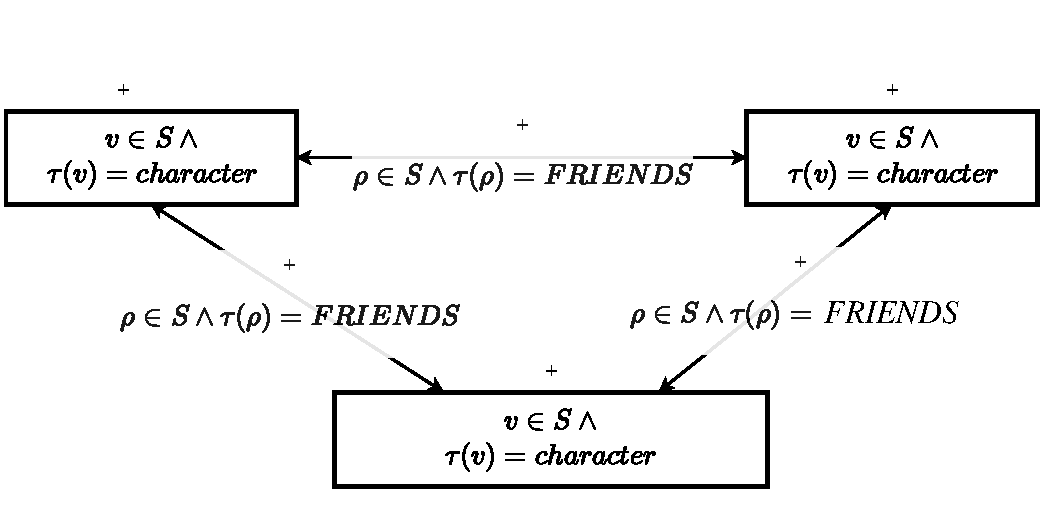
\includegraphics[width=\columnwidth]{png/PQG3.pdf}
    \end{center}
    \caption{%
      Query 2
    }%
    \label{pqg3}
\end{figure}

Query 2 (Figure \ref{pqg3}) outlines a cyclic query that utilises \texttt{FRIENDS} relationships. It will be verified on any subgraph containing three characters who are friends with each other (for example, the subgraph formed by \texttt{Hans Solo}, \texttt{Chewbaka}, \texttt{Princess Leia} and the \texttt{FRIENDS} relationships between them in Figure \ref{starwars}).

\begin{figure}[h]
    \begin{center}
        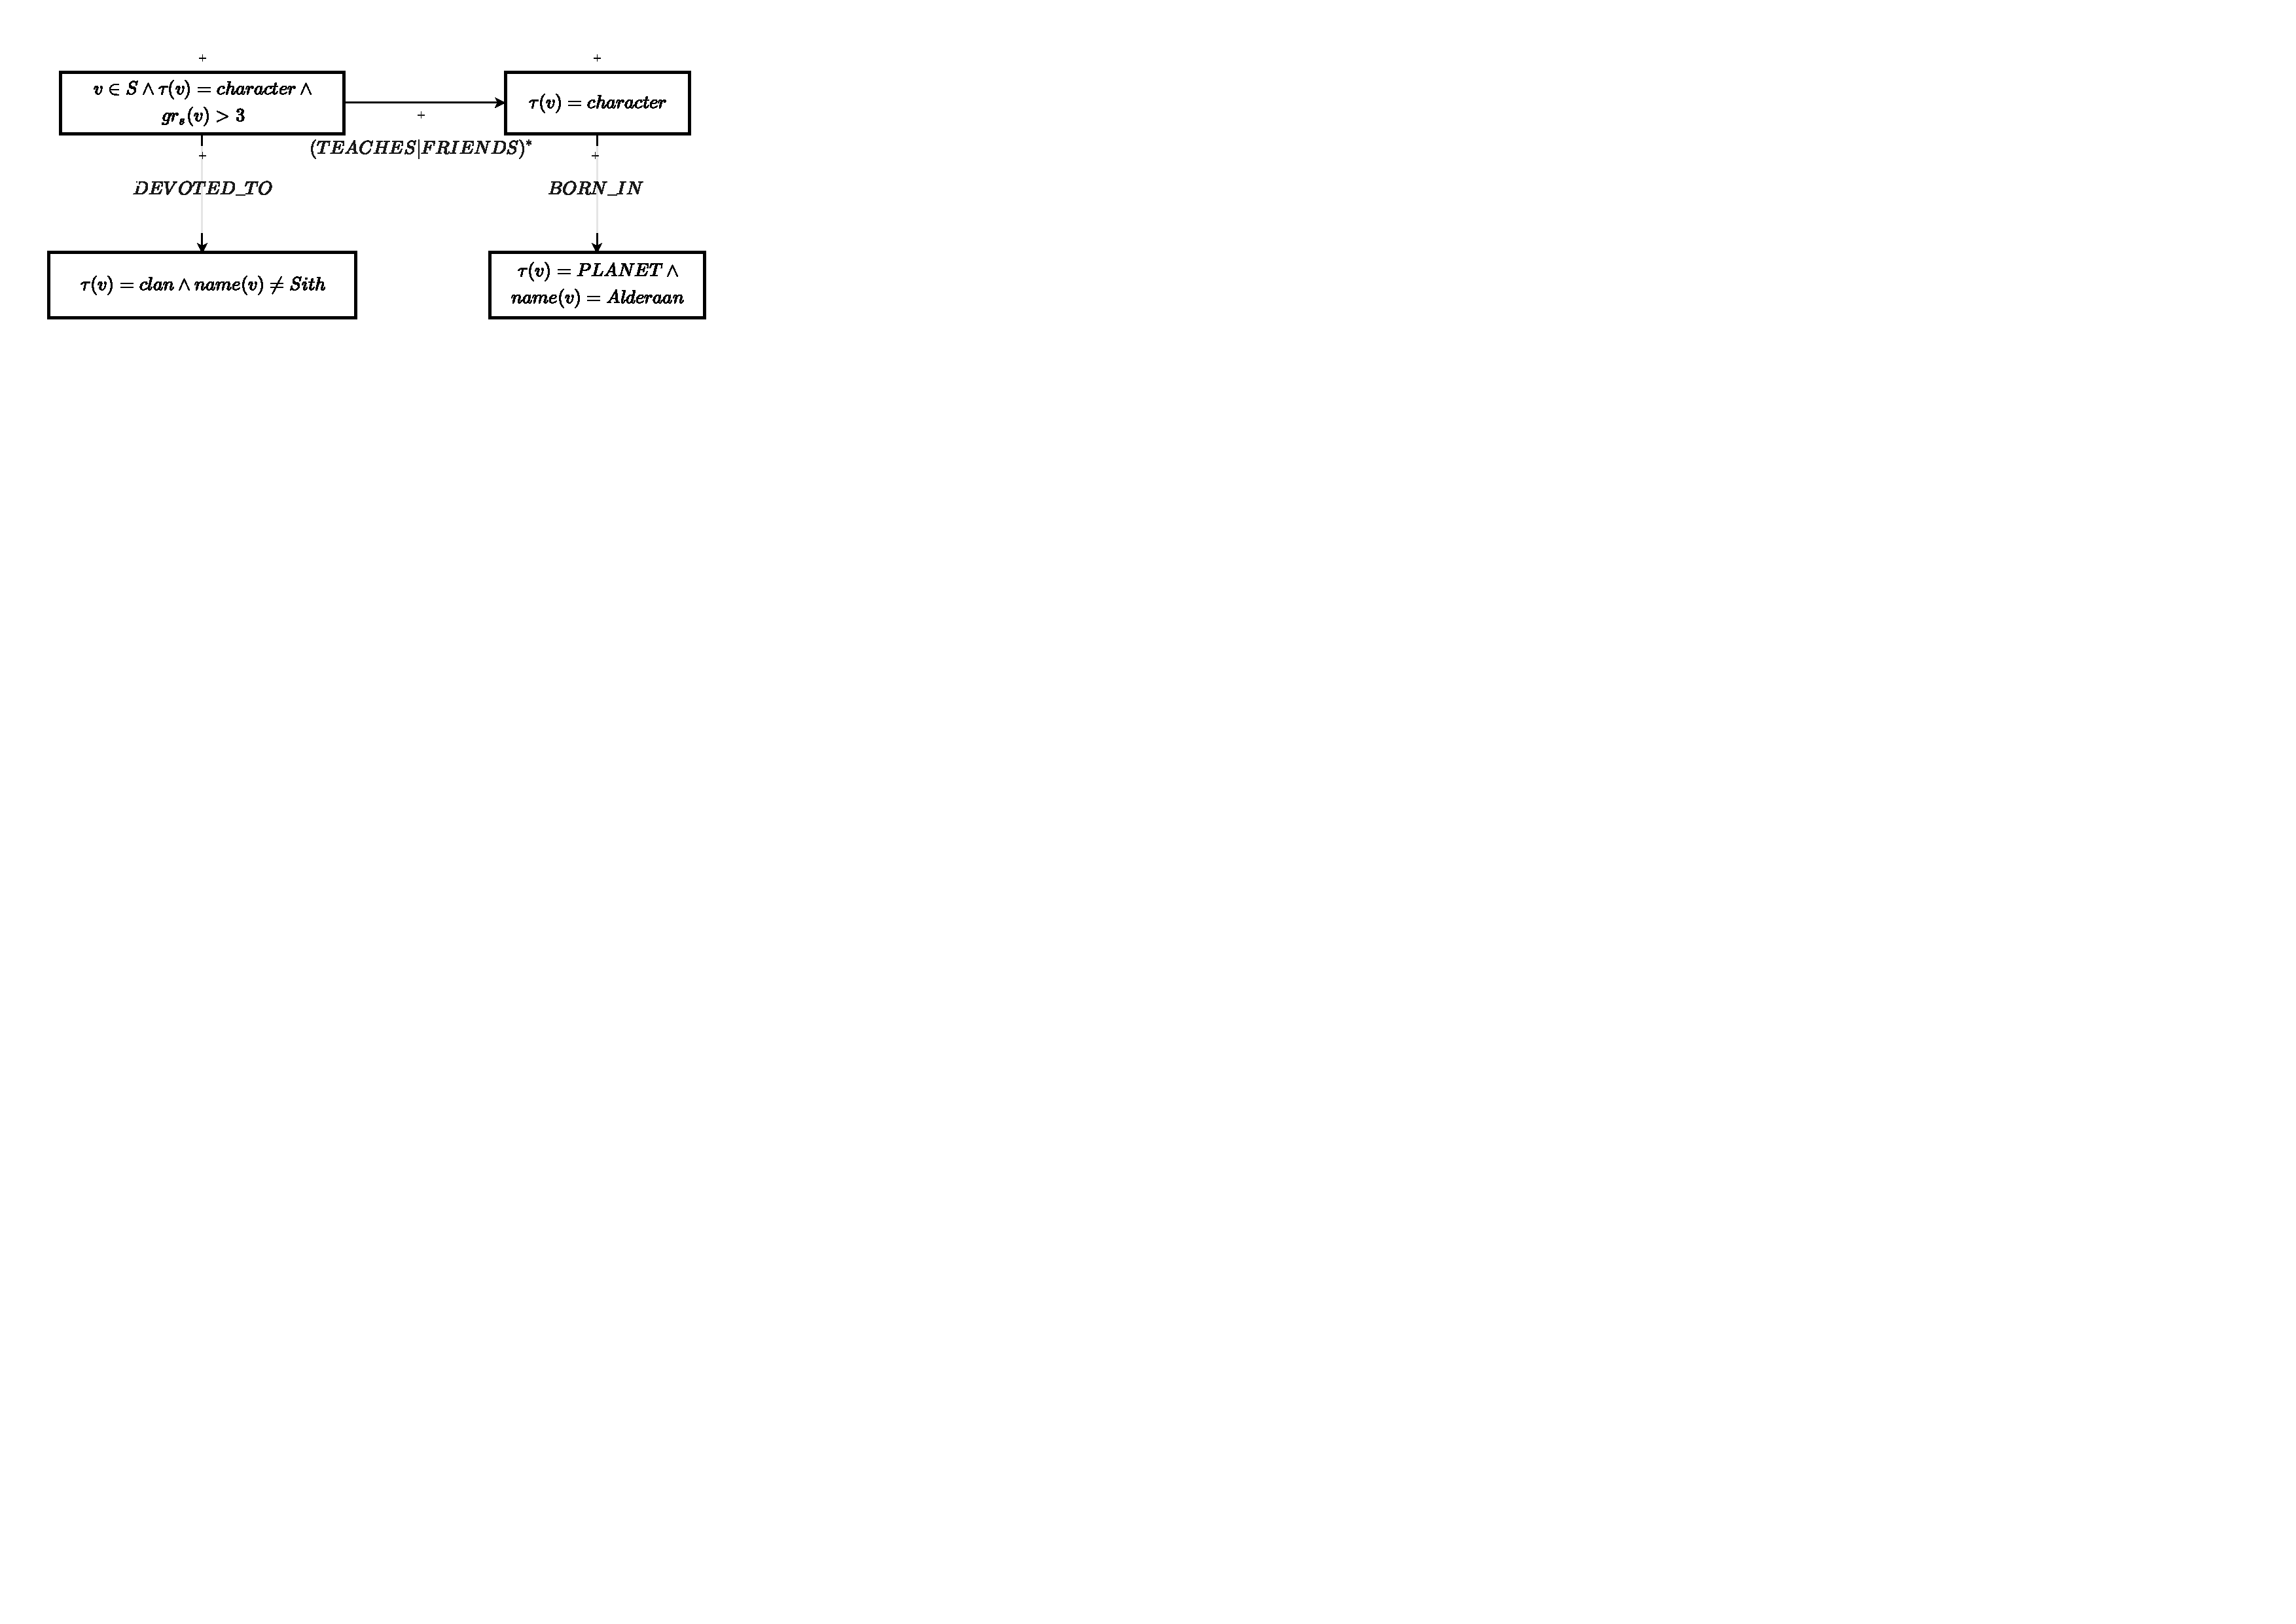
\includegraphics[width=\columnwidth]{png/PQG4.pdf}
    \end{center}
    \caption{%
        Query 3
    }%
    \label{pqg4}
\end{figure}

Query 3 (Figure \ref{pqg4}) can be interpreted as follows: \textit{A character with more than 3 outgoing relationships, not belonging to the Sith clan, connected through a path consisting of any number of FRIENDS and TEACHES relationships with an individual from Alderaan.} In this scenario, a regular expression has been employed to denote a path consisting of an unspecified amount of \texttt{FRIENDS} and \texttt{TEACHES} relationships. Additionally, an auxiliary function, $gr_s(v) \in L$, has been utilised to reference the outgoing degree of node $v$. This query will be validated by any subgraph that contains \texttt{Luke} or \texttt{Obi Wan Kenobi}.

\subsection{Computational complexity}
\label{cc}
Query systems based on graph isomorphisms (most of the existing ones) face NP-complete complexity  \citep{karp1975computational,Cook:1971:CTP:800157.805047}.

The preceding section presented our graph query framework that is reliant on logical predicates. In this section, we will demonstrate that the assessment of queries is polynomial, even in the case of cyclic queries. This is achievable by imposing two constraints. First, the length of paths that are illustrated by links in the query is restricted by the constant $k$, and second, the complexity of the predicates used in nodes and edges is polynomial.

To verify $S\models Q$, it is necessary to examine each predicate $Q_n(S)$ linked to all nodes $n \in V_Q$. Furthermore, each predicate $Q_n(S)$ linked to a node in $Q$ requires assessing one $Q_e(v,S)$ predicate for every link $e\in\gamma_Q(n)$. Thus, initially, we shall focus on evaluating the computational complexity linked with the link predicates $Q_e(v,S)$. Subsequently, we shall proceed to examine the complexity associated with the node predicates $Q_n(S)$. Ultimately, we shall exhibit that the query complexity is polynomial.

As previously defined, the computational complexity of evaluating predicates attributed to both nodes and edges within a query $Q$ is polynomial, denoted by $\mathcal{O}(p)$. The predicates $Q_e(v,S)$ related to edges in a query verify the existence of a path $\rho$ in the graph $G$ starting/ending in $v$ that satisfies its own predicate $\theta_e (\rho, S)$ and with the source and destination nodes that satisfy the predicates $\theta_{e^o} (\rho^o , S)$ and $\theta_{e^i} (\rho^i , S)$ respectively. Thus, the complexity involved in evaluating a particular path is $\mathcal{O}(3p) = \mathcal{O}(p)$. 

The computational complexity to verify the existence of a path beginning or ending at a node $v$ in $V$, satisfying the aforementioned criteria, is $\mathcal{O}(p \times |V|^k)$. Here, $|V|^k$ denotes the number of paths that start or end at $v$ under the condition that they are no longer than $k$ in length. As the number of links commencing or ending at a node $n \in V_Q$ is bound by $|E_Q|$, the computational complexity involved in the node predicate $Q_n(S)$ is $\mathcal{O}(p\times |V|^k \times |E_Q|)$. 

Finally, if the query consists of $|V_Q|$ nodes, the complexity of checking the query $Q(S)$ is $\mathcal{O}(p\times |V|^k \times |E_Q| \times |V_Q|)$. It is evident that the constant $k$ (path length bound) significantly impacts the execution of such queries, as it determines the exponent of the complexity.

Efficient operation of a graph query framework is crucial when dealing with large-scale data sets that are commonly found in real-world applications. Notably, when such a system is employed as the kernel of relational machine learning algorithms, as we will demonstrate in the following section, the ability to perform query operations in polynomial time, even for cyclic queries, is fundamental.

\section{Relational machine learning}
\label{rml}

In this section, we shall leverage the advantages of the framework presented to acquire relational classifiers on graph data sets. To elaborate, we shall initiate from a labelled subgraph set within a graph data set then develop a pattern search technique founded on information gain to obtain typical patterns for each subgraph class.

\subsection{Information-gain pattern mining}
\label{algorithm}

To obtain characteristic patterns of subgraph classes using the previous graph query framework, a top-down decision tree induction will be conducted to explore the pattern space. Within the trees' internal nodes, graph queries will serve as test tools. The best refinement sets will be identified during the tree construction process, resulting in queries that define classes within the graph dataset. 

The training set, $\mathcal{L}$, consists of pairs $(S_i, y_i)$, where $S_i$ denotes a subgraph of $G$ and $y_i$ represents its associated class. Every node $n$ in the resulting decision tree is linked to:
 
\begin{itemize}
\item a subset of the training set: $\mathcal{L}_n \subseteq \mathcal{L}$, 
\item a query $Q_n$ such that: $\forall S \in \mathcal {L}_n (S \vDash Q_n)$.
\end{itemize}

The procedure for tree learning is standard: a tree is initialized comprising one node (the root) linked to the entire set of training, $\mathcal{L}$. The initial query, $ Q_0 $, corresponds to all its constituents ($\forall S \in \mathcal{L}, S \vDash Q_0$). The subsequent stage involves determining which refinement set generates the maximum information gain while separating $\mathcal{L}$, and applying it to $ Q_0 $. For each query in the refinement set, a corresponding child node is created, and $\mathcal{L}$ samples are transmitted through it. A child with a matching associated query is guaranteed to exist since it is a refinement set of $Q_0$. The recursive process continues for each new node until a stop condition is met. At that point, the node becomes a leaf associated with a class. Note that the decision trees derived from this approach are not predominantly binary, unlike the prevalent trees in the literature. 

\subsection{Relational tree learning examples}
\label{kd}

Here, we introduce some practical instances to demonstrate the process of performing relational learning by using the query framework and refinement sets. The refinement operations will be as mentioned in Section \ref{refs}. A critical factor is that all subgraphs in a decision node belong to the same class, which we require as the stopping condition. Initially, we will focus on node classification problems before proceeding to classify more intricate structures. 

Consider the small social network illustrated in Figure \ref{grafo1}, portraying users and items in a graph. The objective is to classify the nodes based on the patterns extracted from the dataset.

\begin{figure}[h!]
  \centering
  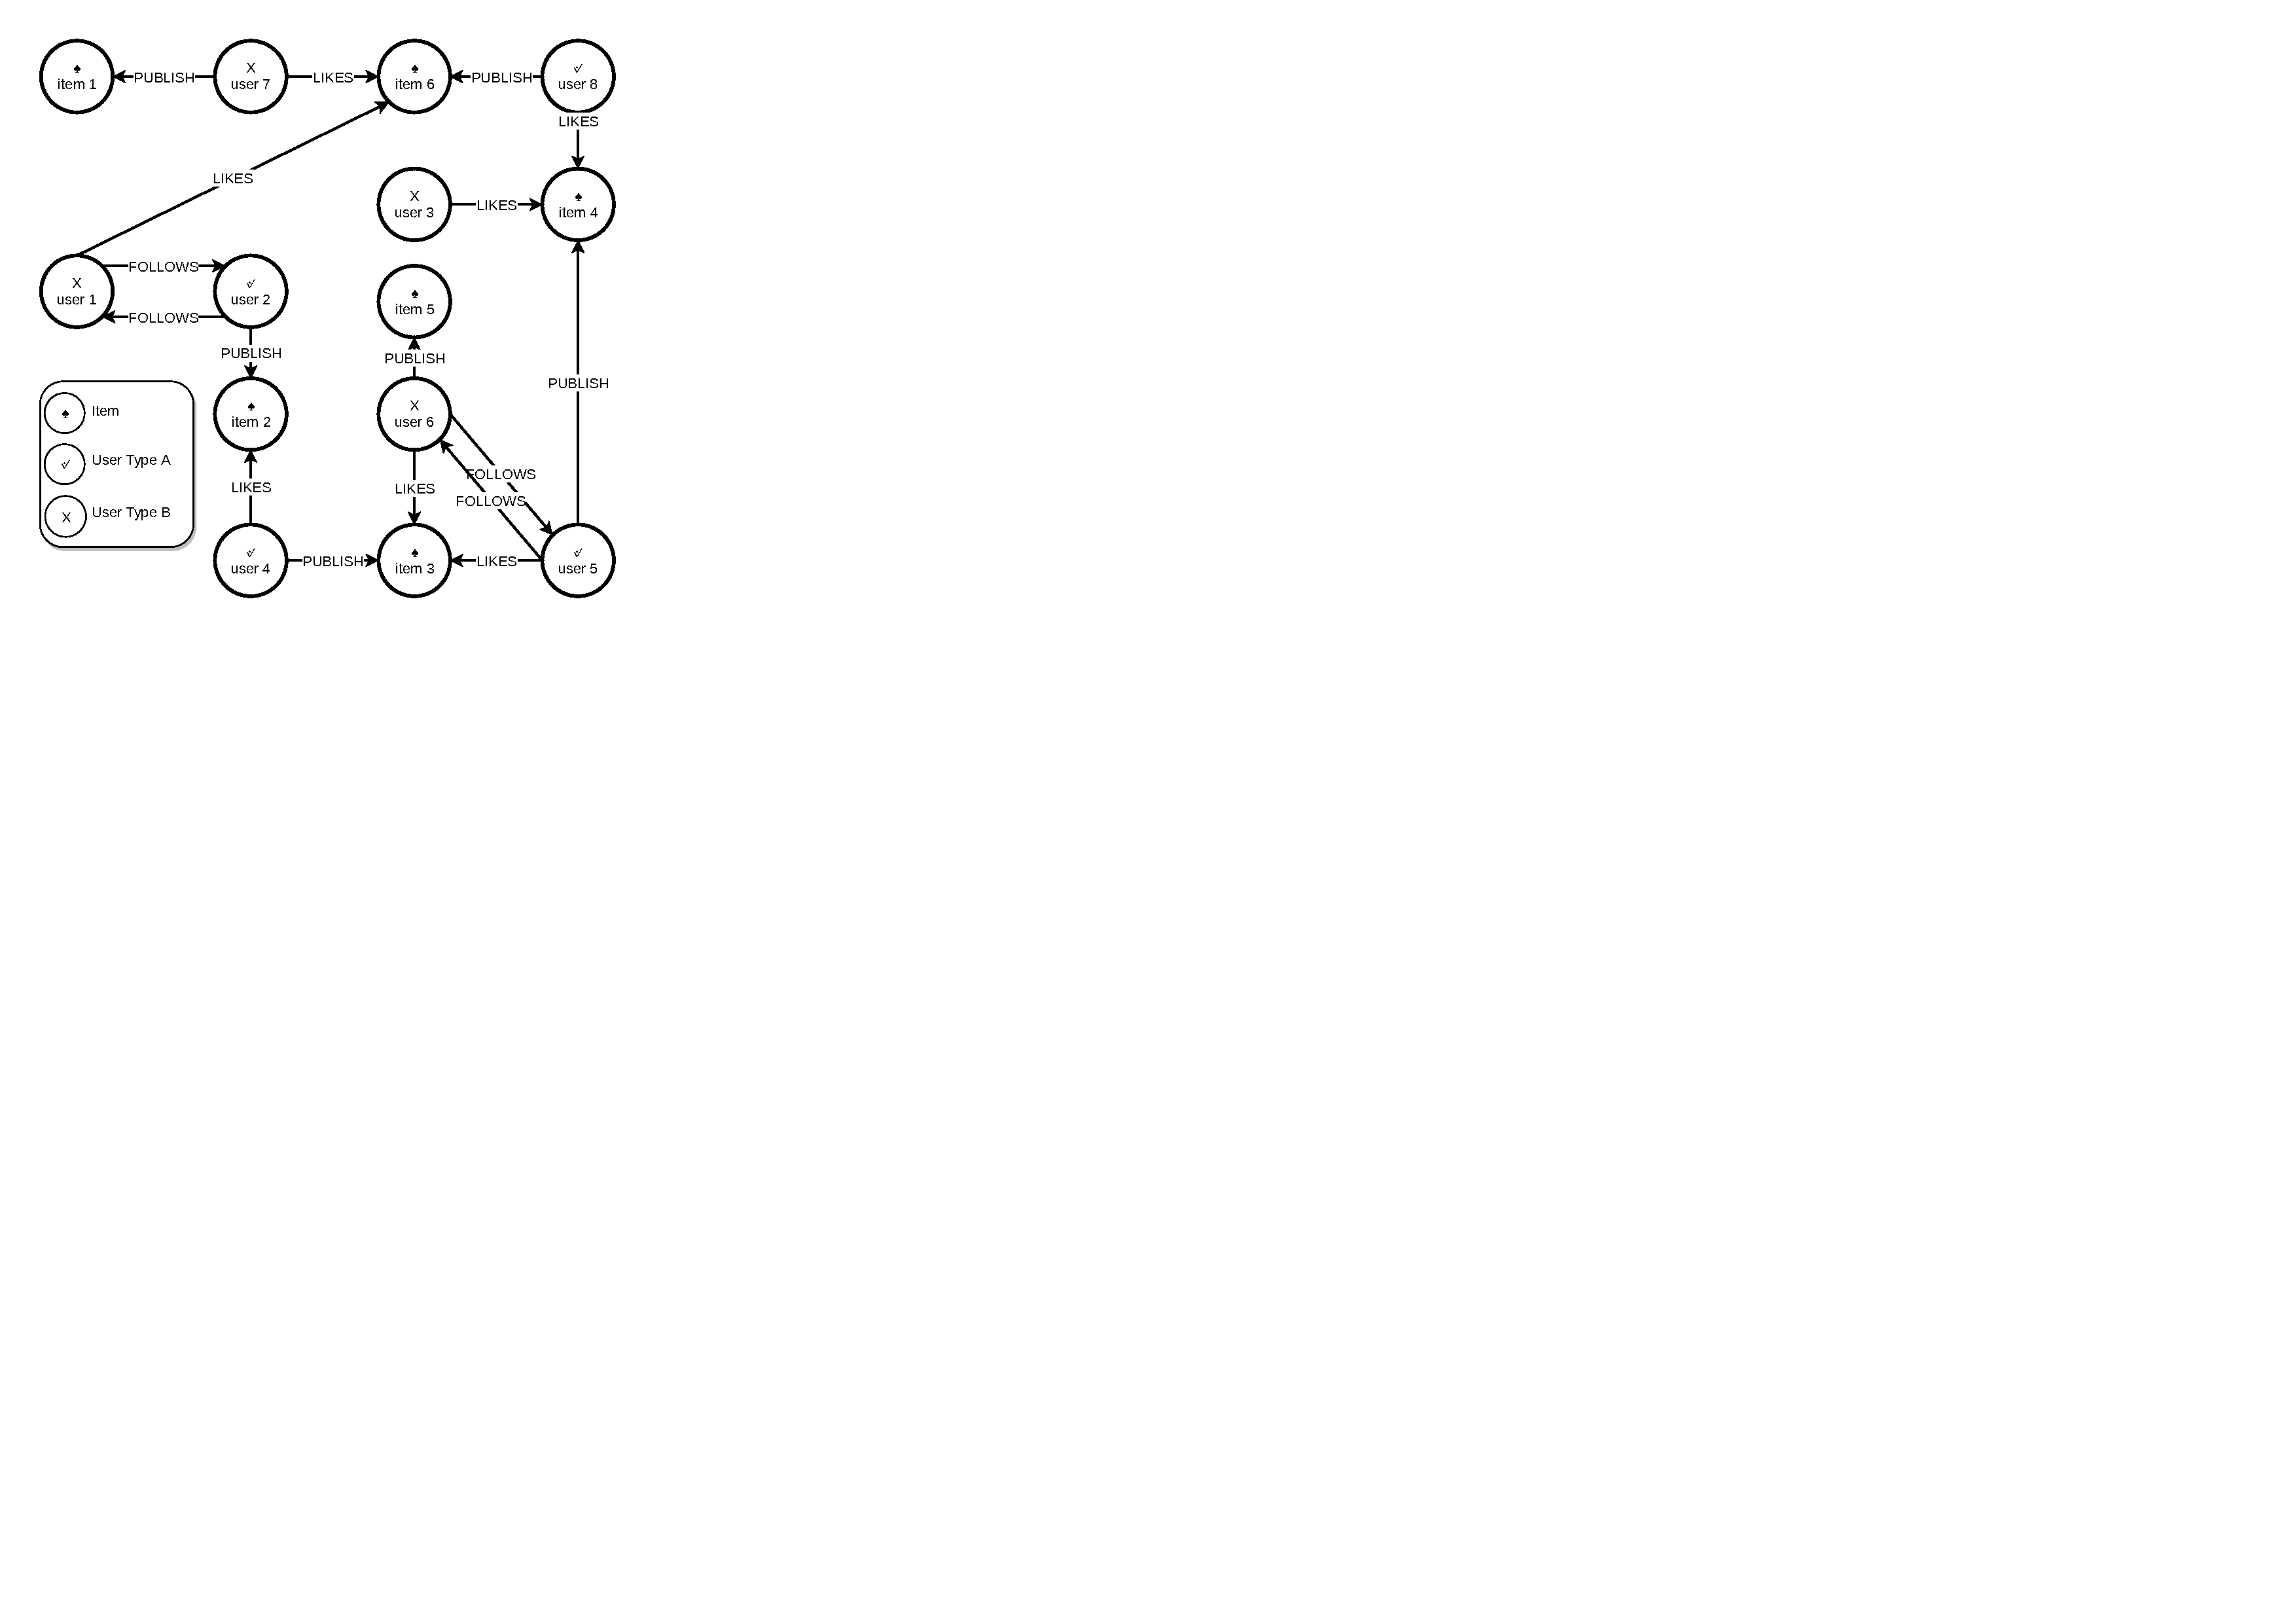
\includegraphics[scale=0.6]{png/FIG8.pdf}
  \caption{Social Network toy}
  \label{grafo1}
\end{figure}

Beginning with a training set composed of all nodes in the graph, Figure \ref{social1} displays the relational decision tree acquired through the process elucidated in Section \ref{algorithm}. Negative nodes/edges are identified with a cross, while nodes with predicate $\theta(v,S) := v \in S$ are larger and white in hue. This tree accurately assigns types (\texttt{User A}, \texttt{User B}, or \texttt{Item}) to all nodes in the graph by exploiting relational information from the network. Furthermore, on the leaves of the tree, distinctive patterns are acquired for each node type, which can be used to directly assess nodes and clarify future classifications. 

\begin{figure}[h!]
	\centering
	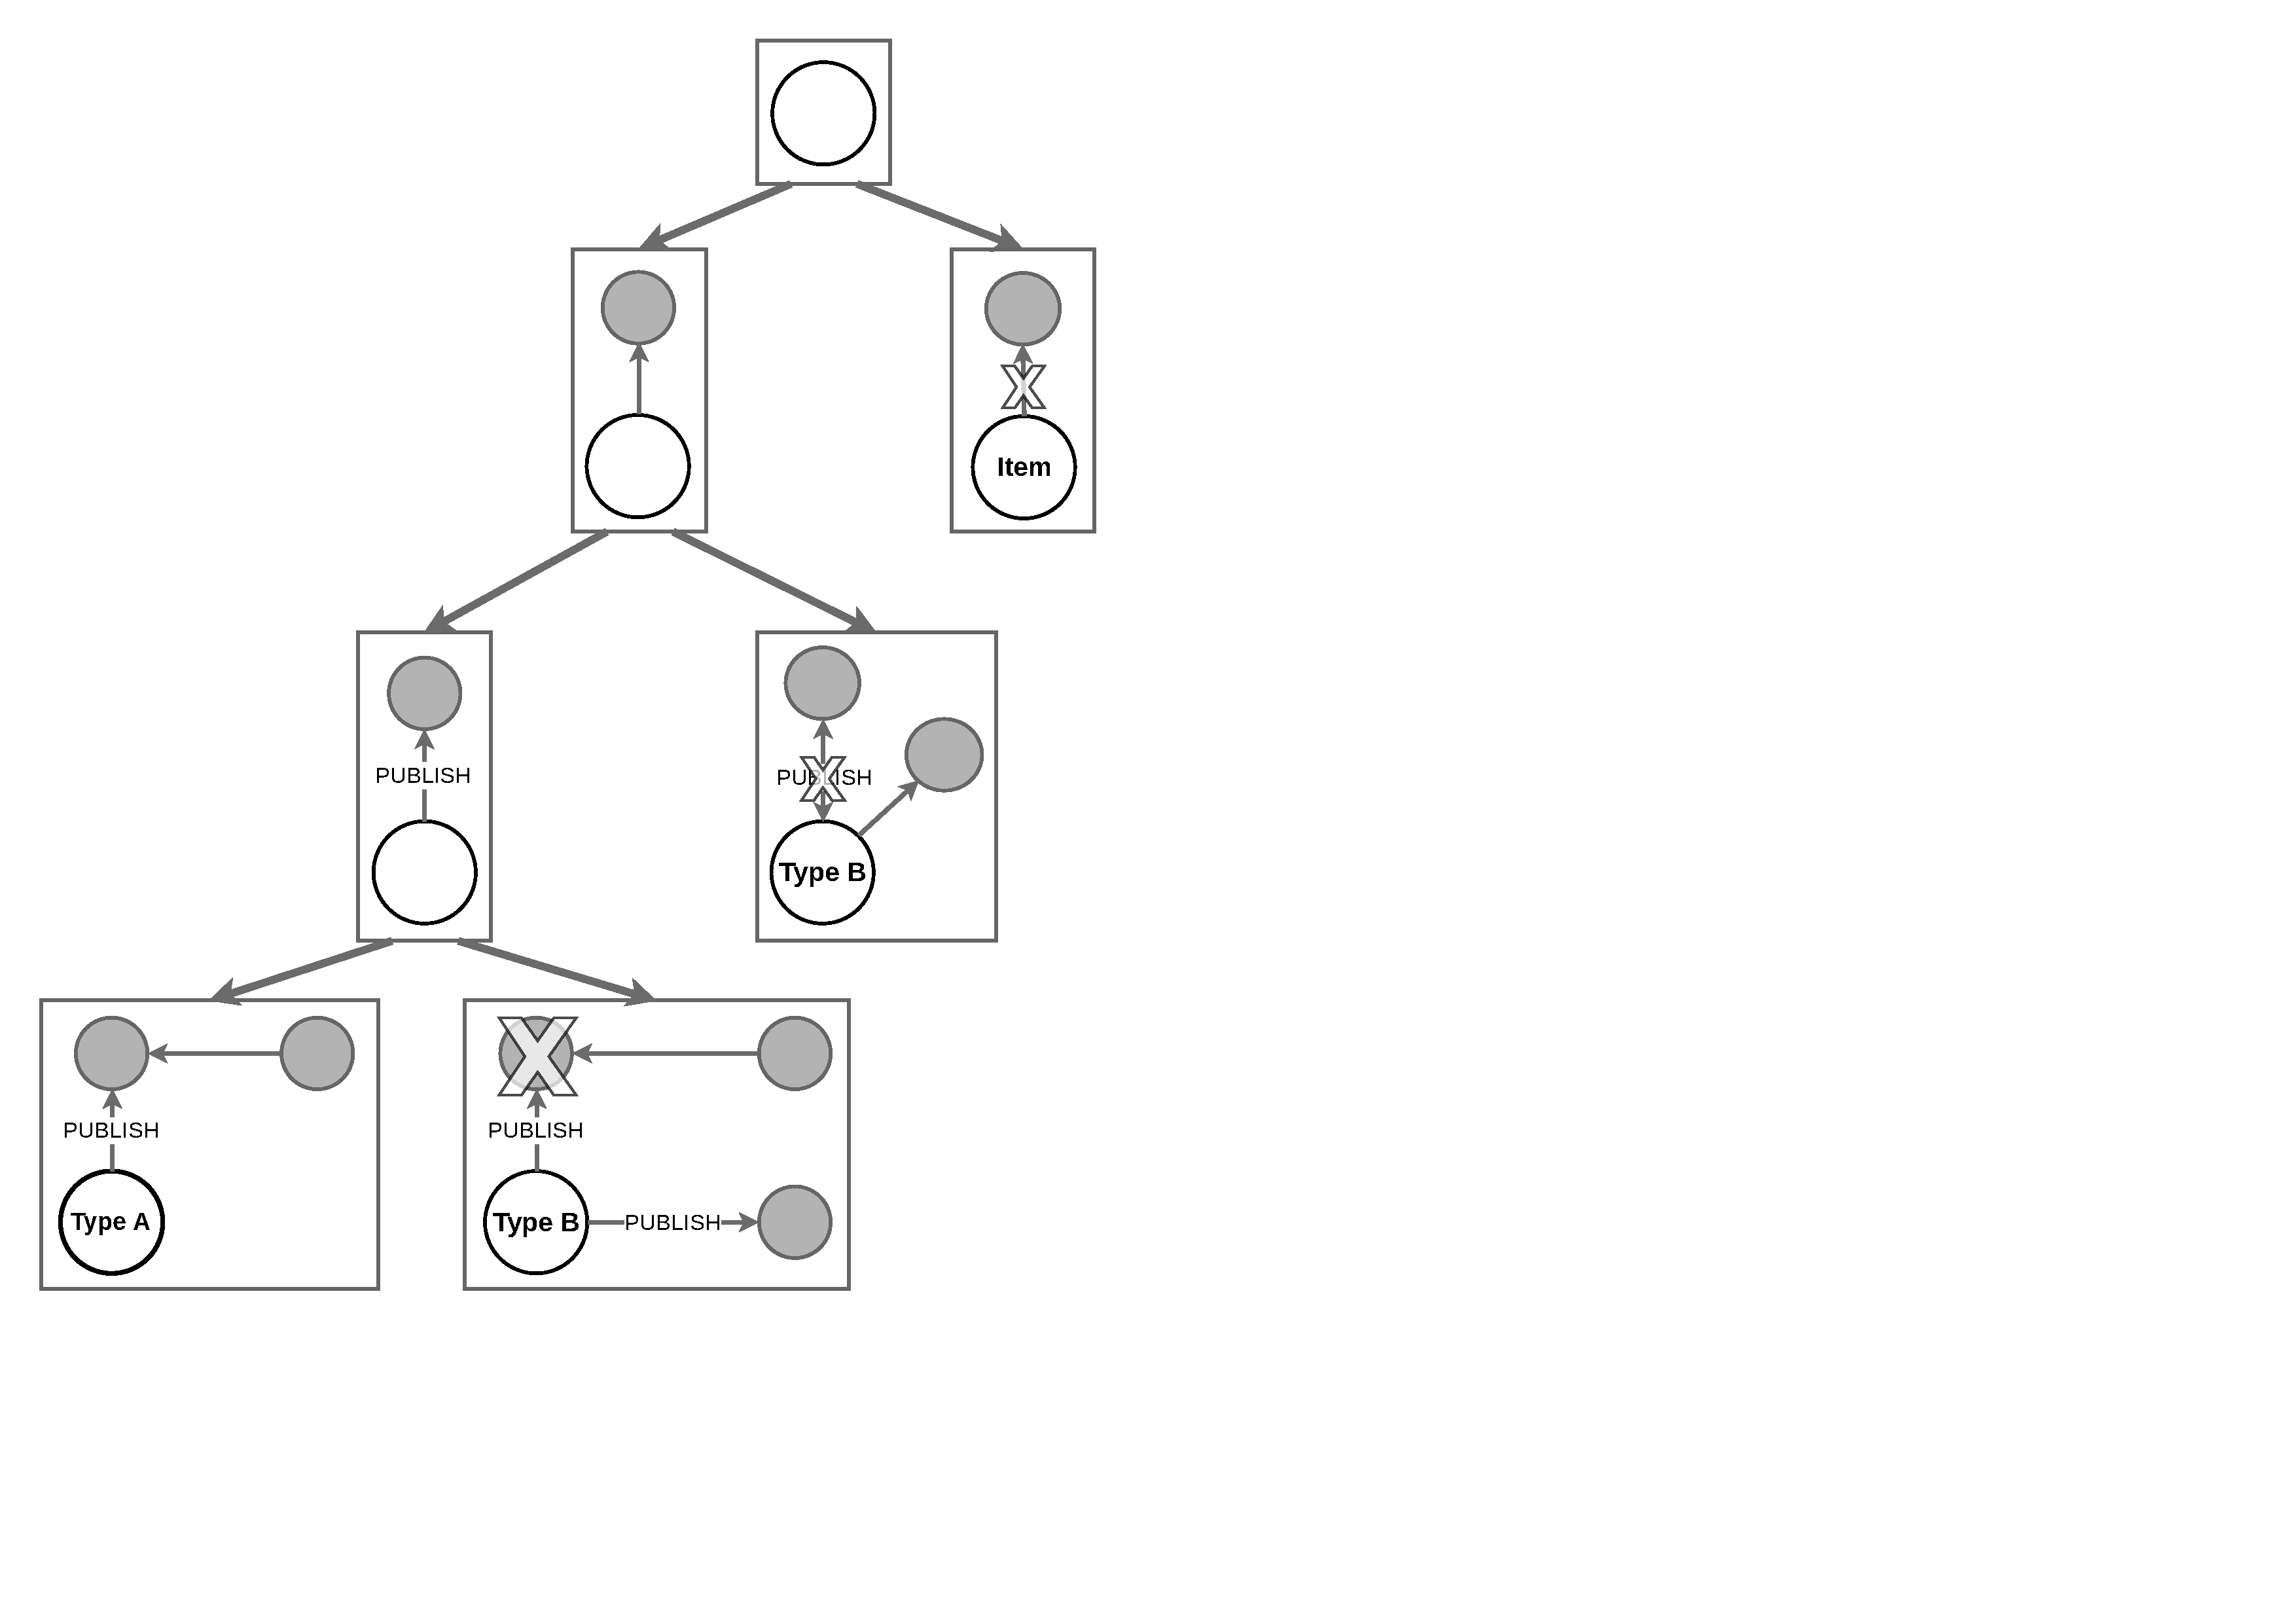
\includegraphics[scale = 0.3]{png/FIG6.pdf}
	\caption{Node type classifier}
	\label{social1}
\end{figure}

Similarly, by utilizing each character node in the Star Wars toy graph (Figure \ref{starwars}) and the corresponding \texttt{specie} property as a training dataset, the relational decision tree shown in Figure \ref{droid} categorizes and explains each character's species in the graph. The leaf patterns of the tree characterize each species: human characters are born friends of \texttt{Luke}, while droids are unborn friends of \texttt{Luke}, wookies are those born in \texttt{Kashyyk}, etc.

\begin{figure}[htb]
    \begin{center}
        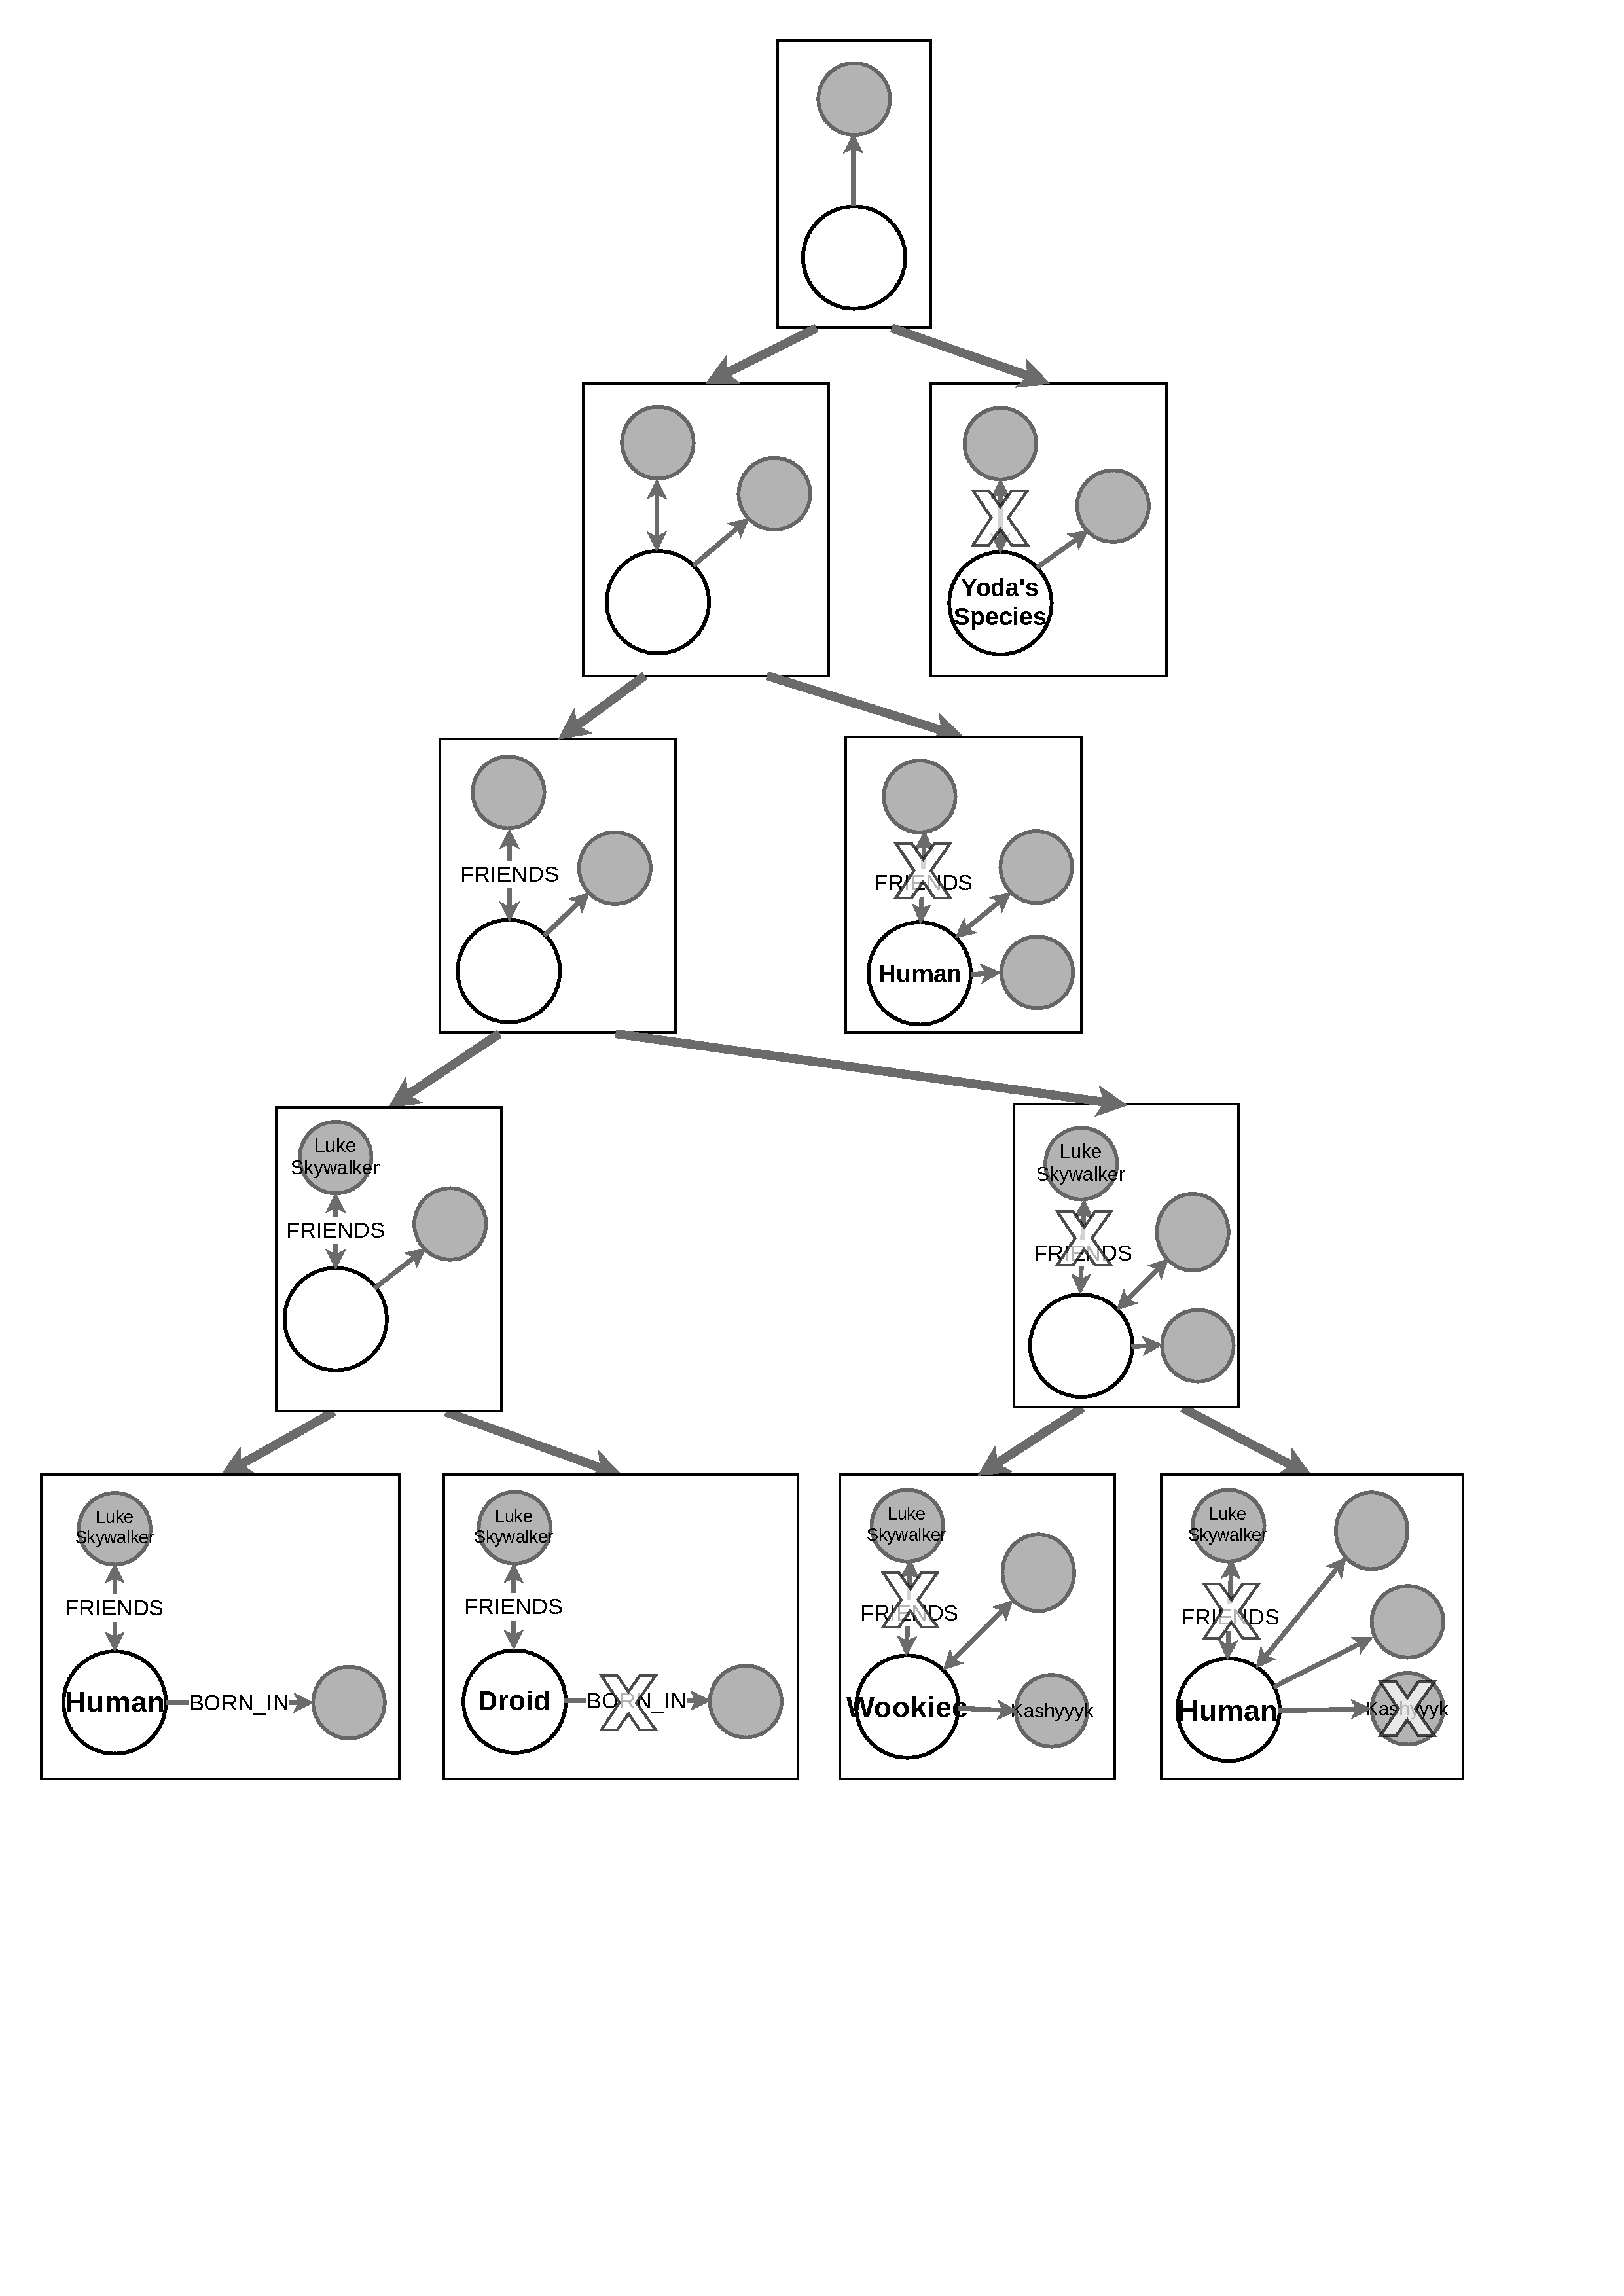
\includegraphics[scale=0.3]{png/FIG7.pdf}
    \end{center}
	\caption{Character specie classifier}
	    \label{droid}
\end{figure}

%As an example of structure classification problem, let us consider the training set composed by pairs master-apprentice connected by a \texttt{TEACHES} relationship in Starwars toy graph in order to distinguish pairs devotee of the same side from those devotee of different sides. Figure \ref{ts} shows the relational decision tree produced by our method. The leftmost leaf provide an explanation for the positive class samples, while the rest of the leafs explain the negative class.
%
%\begin{figure}[htb]
%    \begin{center}
%        \includegraphics[width=\columnwidth]{png/arbolMAStarwars.pdf}
%    \end{center}
%	\caption{Same side Master-Apprentice classifier.}
%	    \label{ts}
%\end{figure}

\section{Conclusions and future work}
\label{cafw}

The paper's main contribution lies in a novel framework for graph queries that permits the polynomial cyclic assessment of queries and refinements based on atomic operations. The framework's ability to apply refinements in relational learning processes was also demonstrated. In addition, the presented framework fulfils several essential requirements. The system utilises a consistent grammar for both queries and evaluated structures. It allows the assessment of subgraphs beyond individual nodes and supports cyclic queries within polynomial time (where the length of the query path is limited). The system offers a controlled and automated query construction via refinements, and the refinement sets constitute embedded partitions of the evaluated structure set, making them effective tools for top-down learning techniques.

Graph isomorphism-based query systems exhibit exponential complexity when presented with cyclic queries. Additionally, if a projection is necessary for pattern verification, evaluating the non-existence of specific elements becomes difficult or even impossible. However, the query graph framework offered here assesses the existence/non-existence of paths and nodes in a graph rather than demanding isomorphisms, thus enabling the evaluation of cyclic patterns in polynomial time. 

After conducting an initial and fully functional proof-of-concept implementation, the graph query framework's capabilities have been demonstrated through experimentation. This methodology has been explicitly applied in relational learning procedures, as demonstrated in section \ref{kd}, and the results of these experiments have shown that interesting patterns can be extracted from relational data. This is of great significance in both explainable learning and automatic feature extraction tasks. The results' graphs were obtained via our proof-of-concept implementation on a graph database and employing the \textit{matplotlib} library \citep{hunter}.

Despite the presented query definition utilizing binary graph data sets (rather than hypergraphs), it can be implemented on hypergraph data as well. This is due to the fact that the concept of a path, which connects pairs of nodes, is independent of the edge arity involved. For the sake of simplicity, and due to the absence of true hypergraph databases, our queries have been limited to the binary case. Nevertheless, they can be adapted to more universal cases once the usage of hypergraphs becomes more widespread.

Also, in Section \ref{refs}, a basic and reliable set of refinement operations have been provided. However, they should not be considered the most suitable solution for all types of learning tasks. To achieve complex queries and to prevent plateaus in the pattern space, more complex refinement families can be established. For example, it is possible to combine the operations \emph{ add edge} and \emph{adding property to an edge} into one step, thereby reducing the number of steps required. If executed properly, unifying the refinements based on the frequency of structural occurrences in a graph, for instance, can lead to faster versions of learning algorithms at the expense of covering a broader query space. This work provides theoretical tools to support the accuracy of new refinement families. Future research will focus on developing automated methods to generate refinement sets based on a given learning task and the specific characteristics of the graph dataset. Extracting statistics from the graph data for automatic generation of such sets can result in significant optimizations. 

It is concluded that it is feasible to establish effective techniques for matching graph patterns and learning symbolic relationships, resulting in systematic exploration of the pattern space, a high degree of expressiveness in queries and computational cost of implementations kept in reasonable orders.
%Complexity associated to queries within the proposed framework is polynomial. However, the constant $k$ that limits the length of the paths searched in the graph plays a fundamental role (section \ref{cc}). For this reason, care must be taken to define such a bounding so that the query system remains viable. Being $d$ the number of attributes and $m$ the number of examples, complexity of decision tree learning algorithms belongs to $\mathcal{O}(d \times m \times \log m)$  \citep{witten2016data}. Thus, complexity of our proposed relational decision tree learning algorithm is polynomial too. As efficiency is one of the major problems for this kind of learning techniques, the higher efficiency of the complete relational learning framework presented here may be very promising.

Patterns associated with the leaves in obtained decision trees can be used to characterize subgraph categories. Moreover, the path from the root node to the corresponding leaf of the decision tree for a particular input can be used to justify decisions, a beneficial feature in various sensitive applications as in decision trees. In addition, patterns obtained from the graph learning procedure presented can serve as features in other machine learning methods. Once the patterns have been acquired, they can serve as Boolean features for subgraph modeling, enabling non-relational machine learning methods to learn from them.

Learning of relational decision trees can be utilised by \textit{ensemble} methods (such as Random Forest), and although the explanatory power is diluted when multiple trees are combined, its predictive power can be greatly enhanced. Therefore, it is essential to investigate the probabilistic amalgamation of queries to generate patterns that can be interpreted as probabilistic decision tools. 

Furthermore, while a relational decision tree learning technique has been employed, additional machine learning algorithms can be evaluated alongside this query framework to investigate more opportunities for relational learning.

\section*{Acknowledgements}


\vspace{6pt} 

%%%%%%%%%%%%%%%%%%%%%%%%%%%%%%%%%%%%%%%%%%
%% optional
%\supplementary{The following supporting information can be downloaded at:  \linksupplementary{s1}, Figure S1: title; Table S1: title; Video S1: title.}

% Only for the journal Methods and Protocols:
% If you wish to submit a video article, please do so with any other supplementary material.
% \supplementary{The following supporting information can be downloaded at: \linksupplementary{s1}, Figure S1: title; Table S1: title; Video S1: title. A supporting video article is available at doi: link.}

%%%%%%%%%%%%%%%%%%%%%%%%%%%%%%%%%%%%%%%%%%
%\authorcontributions{For research articles with several authors, a short paragraph specifying their individual contributions must be provided. The following statements should be used ``Conceptualization, X.X. and Y.Y.; methodology, X.X.; software, X.X.; validation, X.X., Y.Y. and Z.Z.; formal analysis, X.X.; investigation, X.X.; resources, X.X.; data curation, X.X.; writing---original draft preparation, X.X.; writing---review and editing, X.X.; visualization, X.X.; supervision, X.X.; project administration, X.X.; funding acquisition, Y.Y. All authors have read and agreed to the published version of the manuscript.'', please turn to the  \href{http://img.mdpi.org/data/contributor-role-instruction.pdf}{CRediT taxonomy} for the term explanation. Authorship must be limited to those who have contributed substantially to the work~reported.}

%\funding{Please add: ``This research received no external funding'' or ``This research was funded by NAME OF FUNDER grant number XXX.'' and  and ``The APC was funded by XXX''. Check carefully that the details given are accurate and use the standard spelling of funding agency names at \url{https://search.crossref.org/funding}, any errors may affect your future funding.}

%\institutionalreview{In this section, you should add the Institutional Review Board Statement and approval number, if relevant to your study. You might choose to exclude this statement if the study did not require ethical approval. Please note that the Editorial Office might ask you for further information. Please add “The study was conducted in accordance with the Declaration of Helsinki, and approved by the Institutional Review Board (or Ethics Committee) of NAME OF INSTITUTE (protocol code XXX and date of approval).” for studies involving humans. OR “The animal study protocol was approved by the Institutional Review Board (or Ethics Committee) of NAME OF INSTITUTE (protocol code XXX and date of approval).” for studies involving animals. OR “Ethical review and approval were waived for this study due to REASON (please provide a detailed justification).” OR “Not applicable” for studies not involving humans or animals.}

%\informedconsent{Any research article describing a study involving humans should contain this statement. Please add ``Informed consent was obtained from all subjects involved in the study.'' OR ``Patient consent was waived due to REASON (please provide a detailed justification).'' OR ``Not applicable'' for studies not involving humans. You might also choose to exclude this statement if the study did not involve humans.

%Written informed consent for publication must be obtained from participating patients who can be identified (including by the patients themselves). Please state ``Written informed consent has been obtained from the patient(s) to publish this paper'' if applicable.}

%\dataavailability{We encourage all authors of articles published in MDPI journals to share their research data. In this section, please provide details regarding where data supporting reported results can be found, including links to publicly archived datasets analyzed or generated during the study. Where no new data were created, or where data is unavailable due to privacy or ethical re-strictions, a statement is still required. Suggested Data Availability Statements are available in section “MDPI Research Data Policies” at \url{https://www.mdpi.com/ethics}.} 

\funding{Proyecto PID2019-109152G financiado por MCIN/AEI/10.13039/501100011033}

\acknowledgments{DISARM project - Grant n. PDC2021-121197, and the HORUS project - Grant n. PID2021-126359OB-I00 funded by MCIN/AEI/310.13039/501100011033 and by the “European Union NextGenerationEU/PRTR”}

%\conflictsofinterest{Declare conflicts of interest or state ``The authors declare no conflict of interest.'' Authors must identify and declare any personal circumstances or interest that may be perceived as inappropriately influencing the representation or interpretation of reported research results. Any role of the funders in the design of the study; in the collection, analyses or interpretation of data; in the writing of the manuscript; or in the decision to publish the results must be declared in this section. If there is no role, please state ``The funders had no role in the design of the study; in the collection, analyses, or interpretation of data; in the writing of the manuscript; or in the decision to publish the~results''.} 

%%%%%%%%%%%%%%%%%%%%%%%%%%%%%%%%%%%%%%%%%%
%% Optional


%\section[\appendixname~\thesection]{}
%All appendix sections must be cited in the main text. In the appendices, Figures, Tables, etc. should be labeled, starting with ``A''---e.g., Figure A1, Figure A2, etc.

%%%%%%%%%%%%%%%%%%%%%%%%%%%%%%%%%%%%%%%%%%
\begin{adjustwidth}{-\extralength}{0cm}
%\printendnotes[custom] % Un-comment to print a list of endnotes

\reftitle{References}

% Please provide either the correct journal abbreviation (e.g. according to the “List of Title Word Abbreviations” http://www.issn.org/services/online-services/access-to-the-ltwa/) or the full name of the journal.
% Citations and References in Supplementary files are permitted provided that they also appear in the reference list here. 

%=====================================
% References, variant A: external bibliography
%=====================================
%\bibliography{your_external_BibTeX_file}

%=====================================
% References, variant B: internal bibliography
%=====================================
\begin{thebibliography}{31}
\expandafter\ifx\csname natexlab\endcsname\relax\def\natexlab#1{#1}\fi
\providecommand{\url}[1]{\texttt{#1}}
\providecommand{\href}[2]{#2}
\providecommand{\path}[1]{#1}
\providecommand{\DOIprefix}{doi:}
\providecommand{\ArXivprefix}{arXiv:}
\providecommand{\URLprefix}{URL: }
\providecommand{\Pubmedprefix}{pmid:}
\providecommand{\doi}[1]{\href{http://dx.doi.org/#1}{\path{#1}}}
\providecommand{\Pubmed}[1]{\href{pmid:#1}{\path{#1}}}
\providecommand{\bibinfo}[2]{#2}
\ifx\xfnm\relax \def\xfnm[#1]{\unskip,\space#1}\fi
%Type = Article
\bibitem[{Almagro{-}Blanco \&
  Sancho{-}Caparrini(2017)}]{DBLP:journals/corr/abs-1708-03734}
\bibinfo{author}{Almagro{-}Blanco, P.}, \& \bibinfo{author}{Sancho{-}Caparrini,
  F.} (\bibinfo{year}{2017}).
\newblock \bibinfo{title}{Generalized graph pattern matching}.
\newblock {\it \bibinfo{journal}{CoRR}\/},  {\it
  \bibinfo{volume}{abs/1708.03734}\/}. \URLprefix
  \url{http://arxiv.org/abs/1708.03734}.
  \href{http://arxiv.org/abs/1708.03734}{\tt arXiv:1708.03734}.
%Type = Inproceedings
\bibitem[{Barcel{\'o} et~al.(2011)Barcel{\'o}, Libkin \& Reutter}]{Barcelo}
\bibinfo{author}{Barcel{\'o}, P.}, \bibinfo{author}{Libkin, L.}, \&
  \bibinfo{author}{Reutter, J.~L.} (\bibinfo{year}{2011}).
\newblock \bibinfo{title}{Querying graph patterns}.
\newblock In {\it \bibinfo{booktitle}{Proceedings of the Thirtieth ACM
  SIGMOD-SIGACT-SIGART Symposium on Principles of Database Systems}\/} PODS '11
  (pp. \bibinfo{pages}{199--210}).
\newblock \bibinfo{address}{New York, NY, USA}: \bibinfo{publisher}{ACM}.
\newblock \URLprefix \url{http://doi.acm.org/10.1145/1989284.1989307}.
  \DOIprefix\doi{10.1145/1989284.1989307}.
%Type = Article
\bibitem[{Blockeel \& Raedt(1998)}]{BLOCKEEL1998285}
\bibinfo{author}{Blockeel, H.}, \& \bibinfo{author}{Raedt, L.~D.}
  (\bibinfo{year}{1998}).
\newblock \bibinfo{title}{Top-down induction of first-order logical decision
  trees}.
\newblock {\it \bibinfo{journal}{Artificial Intelligence}\/},  {\it
  \bibinfo{volume}{101}\/}, \bibinfo{pages}{285--297}. \URLprefix
  \url{http://www.sciencedirect.com/science/article/pii/S0004370298000344}.
  \DOIprefix\doi{10.1016/S0004-3702(98)00034-4}.
%Type = Incollection

\bibitem[{Bonifati, Angela and Fletcher, George and Voigt, Hannes and Yakovets, Nikolay and Jagadish, H. V.}]{Bonifati}
\bibinfo{author}{Bonifati, A.} \bibinfo{author}{Fletcher, G.}\bibinfo{author}{Voigt, H.}\bibinfo{author}{Yakovets, N.}\bibinfo{author}{Jagadish, H. V.} (\bibinfo{year}{2018}
\newblock \bibinfo{title}{Querying Graphs}
\newblock \bibinfo{publisher}{Morgan \& Claypool Publishers}

\bibitem[{Bordes et~al.(2013)Bordes, Usunier, Garcia-Duran, Weston \&
  Yakhnenko}]{transe}
\bibinfo{author}{Bordes, A.}, \bibinfo{author}{Usunier, N.},
  \bibinfo{author}{Garcia-Duran, A.}, \bibinfo{author}{Weston, J.}, \&
  \bibinfo{author}{Yakhnenko, O.} (\bibinfo{year}{2013}).
\newblock \bibinfo{title}{Translating embeddings for modeling multi-relational
  data}.
\newblock In \bibinfo{editor}{C.~J.~C. Burges}, \bibinfo{editor}{L.~Bottou},
  \bibinfo{editor}{M.~Welling}, \bibinfo{editor}{Z.~Ghahramani}, \&
  \bibinfo{editor}{K.~Q. Weinberger} (Eds.), {\it \bibinfo{booktitle}{Advances
  in Neural Information Processing Systems 26}\/} (pp.
  \bibinfo{pages}{2787--2795}).
\newblock \bibinfo{publisher}{Curran Associates, Inc.}
\newblock \URLprefix
  \url{http://papers.nips.cc/paper/5071-translating-embeddings-for-modeling-multi-relational-data.pdf}.

  
%Type = Article
\bibitem[{Brynjolfsson \& Mitchell(2017)}]{brynjolfsson2017can}
\bibinfo{author}{Brynjolfsson, E.}, \& \bibinfo{author}{Mitchell, T.}
  (\bibinfo{year}{2017}).
\newblock \bibinfo{title}{What can machine learning do? workforce
  implications}.
\newblock {\it \bibinfo{journal}{Science}\/},  {\it \bibinfo{volume}{358}\/},
  \bibinfo{pages}{1530--1534}.
%Type = Article
\bibitem[{Camacho et~al.(2011)Camacho, Pereira, Costa, Fonseca, Adriano,
  Sim{\~o}es \& Brito}]{camacho2011relational}
\bibinfo{author}{Camacho, R.}, \bibinfo{author}{Pereira, M.},
  \bibinfo{author}{Costa, V.~S.}, \bibinfo{author}{Fonseca, N.~A.},
  \bibinfo{author}{Adriano, C.}, \bibinfo{author}{Sim{\~o}es, C.~J.}, \&
  \bibinfo{author}{Brito, R.~M.} (\bibinfo{year}{2011}).
\newblock \bibinfo{title}{A relational learning approach to structure-activity
  relationships in drug design toxicity studies}.
\newblock {\it \bibinfo{journal}{Journal of integrative bioinformatics}\/},
  {\it \bibinfo{volume}{8}\/}, \bibinfo{pages}{176--194}.
%Type = Inproceedings
\bibitem[{Chang et~al.(2014)Chang, Yih, Yang \& Meek}]{typed}
\bibinfo{author}{Chang, K.-W.}, \bibinfo{author}{Yih, S. W.-t.},
  \bibinfo{author}{Yang, B.}, \& \bibinfo{author}{Meek, C.}
  (\bibinfo{year}{2014}).
\newblock \bibinfo{title}{Typed tensor decomposition of knowledge bases for
  relation extraction}.
\newblock In {\it \bibinfo{booktitle}{Proceedings of the 2014 Conference on
  Empirical Methods in Natural Language Processing}\/}.
\newblock \bibinfo{publisher}{ACL -- Association for Computational
  Linguistics}.
\newblock \URLprefix
  \url{https://www.microsoft.com/en-us/research/publication/typed-tensor-decomposition-of-knowledge-bases-for-relation-extraction/}.
%Type = Inproceedings
\bibitem[{Consens \& Mendelzon(1990)}]{graphlog}
\bibinfo{author}{Consens, M.~P.}, \& \bibinfo{author}{Mendelzon, A.~O.}
  (\bibinfo{year}{1990}).
\newblock \bibinfo{title}{Graphlog: A visual formalism for real life
  recursion}.
\newblock In {\it \bibinfo{booktitle}{Proceedings of the Ninth ACM
  SIGACT-SIGMOD-SIGART Symposium on Principles of Database Systems}\/} PODS '90
  (pp. \bibinfo{pages}{404--416}).
\newblock \bibinfo{address}{New York, NY, USA}: \bibinfo{publisher}{ACM}.
\newblock \URLprefix \url{http://doi.acm.org/10.1145/298514.298591}.
  \DOIprefix\doi{10.1145/298514.298591}.
%Type = Inproceedings
\bibitem[{Cook(1971)}]{Cook:1971:CTP:800157.805047}
\bibinfo{author}{Cook, S.~A.} (\bibinfo{year}{1971}).
\newblock \bibinfo{title}{The complexity of theorem-proving procedures}.
\newblock In {\it \bibinfo{booktitle}{Proceedings of the Third Annual ACM
  Symposium on Theory of Computing}\/} STOC '71 (pp.
  \bibinfo{pages}{151--158}).
\newblock \bibinfo{address}{New York, NY, USA}: \bibinfo{publisher}{ACM}.
\newblock \URLprefix \url{http://doi.acm.org/10.1145/800157.805047}.
  \DOIprefix\doi{10.1145/800157.805047}.
%Type = Inproceedings
\bibitem[{Dong et~al.(2014)Dong, Gabrilovich, Heitz, Horn, Lao, Murphy,
  Strohmann, Sun \& Zhang}]{webscale}
\bibinfo{author}{Dong, X.}, \bibinfo{author}{Gabrilovich, E.},
  \bibinfo{author}{Heitz, G.}, \bibinfo{author}{Horn, W.},
  \bibinfo{author}{Lao, N.}, \bibinfo{author}{Murphy, K.},
  \bibinfo{author}{Strohmann, T.}, \bibinfo{author}{Sun, S.}, \&
  \bibinfo{author}{Zhang, W.} (\bibinfo{year}{2014}).
\newblock \bibinfo{title}{Knowledge vault: A web-scale approach to
  probabilistic knowledge fusion}.
\newblock In {\it \bibinfo{booktitle}{Proceedings of the 20th ACM SIGKDD
  International Conference on Knowledge Discovery and Data Mining}\/} KDD '14
  (pp. \bibinfo{pages}{601--610}).
\newblock \bibinfo{address}{New York, NY, USA}: \bibinfo{publisher}{ACM}.
\newblock \URLprefix \url{http://doi.acm.org/10.1145/2623330.2623623}.
  \DOIprefix\doi{10.1145/2623330.2623623}.
%Type = Article
\bibitem[{Fan et~al.(2010)Fan, Li, Ma, Tang, Wu \& Wu}]{Fan}
\bibinfo{author}{Fan, W.}, \bibinfo{author}{Li, J.}, \bibinfo{author}{Ma, S.},
  \bibinfo{author}{Tang, N.}, \bibinfo{author}{Wu, Y.}, \& \bibinfo{author}{Wu,
  Y.} (\bibinfo{year}{2010}).
\newblock \bibinfo{title}{Graph pattern matching: From intractable to
  polynomial time}.
\newblock {\it \bibinfo{journal}{Proc. VLDB Endow.}\/},  {\it
  \bibinfo{volume}{3}\/}, \bibinfo{pages}{264--275}. \URLprefix
  \url{http://dx.doi.org/10.14778/1920841.1920878}.
  \DOIprefix\doi{10.14778/1920841.1920878}.
 
%Type = Article
\bibitem[{Gallagher(2006)}]{matching}
\bibinfo{author}{Gallagher, B.} (\bibinfo{year}{2006}).
\newblock \bibinfo{title}{Matching structure and semantics: A survey on
  graph-based pattern matching}.
\newblock {\it \bibinfo{journal}{AAAI FS}\/},  {\it \bibinfo{volume}{6}\/},
  \bibinfo{pages}{45--53}.
%Type = Article
\bibitem[{García-Jiménez et~al.(2014)García-Jiménez, Pons, Sanchis \&
  Valencia}]{6802366}
\bibinfo{author}{García-Jiménez, B.}, \bibinfo{author}{Pons, T.},
  \bibinfo{author}{Sanchis, A.}, \& \bibinfo{author}{Valencia, A.}
  (\bibinfo{year}{2014}).
\newblock \bibinfo{title}{Predicting protein relationships to human pathways
  through a relational learning approach based on simple sequence features}.
\newblock {\it \bibinfo{journal}{IEEE/ACM Transactions on Computational Biology
  and Bioinformatics}\/},  {\it \bibinfo{volume}{11}\/},
  \bibinfo{pages}{753--765}. \DOIprefix\doi{10.1109/TCBB.2014.2318730}.
%Type = Inbook
\bibitem[{Geamsakul et~al.(2003)Geamsakul, Matsuda, Yoshida, Motoda \&
  Washio}]{Geamsakul2003}
\bibinfo{author}{Geamsakul, W.}, \bibinfo{author}{Matsuda, T.},
  \bibinfo{author}{Yoshida, T.}, \bibinfo{author}{Motoda, H.}, \&
  \bibinfo{author}{Washio, T.} (\bibinfo{year}{2003}).
\newblock \bibinfo{title}{Classifier construction by graph-based induction for
  graph-structured data}.
\newblock In \bibinfo{editor}{K.-Y. Whang}, \bibinfo{editor}{J.~Jeon},
  \bibinfo{editor}{K.~Shim}, \& \bibinfo{editor}{J.~Srivastava} (Eds.), {\it
  \bibinfo{booktitle}{Advances in Knowledge Discovery and Data Mining: 7th
  Pacific-Asia Conference, PAKDD 2003, Seoul, Korea, April 30 -- May 2, 2003
  Proceedings}\/} (pp. \bibinfo{pages}{52--62}).
\newblock \bibinfo{address}{Berlin, Heidelberg}: \bibinfo{publisher}{Springer
  Berlin Heidelberg}.
\newblock \URLprefix \url{http://dx.doi.org/10.1007/3-540-36175-8_6}.
  \DOIprefix\doi{10.1007/3-540-36175-8_6}.
%Type = Book
\bibitem[{Gupta(2015)}]{gupta2015neo4j}
\bibinfo{author}{Gupta, S.} (\bibinfo{year}{2015}).
\newblock {\it \bibinfo{title}{Neo4j Essentials}\/}.
\newblock Community experience distilled.
\newblock \bibinfo{publisher}{Packt Publishing}.
\newblock \URLprefix \url{https://books.google.es/books?id=WJ7NBgAAQBAJ}.
%Type = Inproceedings
\bibitem{de_raedt_2021}
Luc De Raedt, Sebastijan Duman\v{c}i\'{c}, Robin Manhaeve, Giuseppe Marra.
\emph{From Statistical Relational to Neural-Symbolic Artificial Intelligence}.
In \emph{Proceedings of the Twenty-Ninth International Joint Conference on Artificial Intelligence (IJCAI'20)}, 2021.
ISBN: 9780999241165.
Article No.: 688.
Pages: 8.
Yokohama, Japan.
%Type = Inproceedings
\bibitem[{Henzinger et~al.(1995)Henzinger, Henzinger \&
  Kopke}]{henzinger1995computing}
\bibinfo{author}{Henzinger, M.~R.}, \bibinfo{author}{Henzinger, T.~A.}, \&
  \bibinfo{author}{Kopke, P.~W.} (\bibinfo{year}{1995}).
\newblock \bibinfo{title}{Computing simulations on finite and infinite graphs}.
\newblock In {\it \bibinfo{booktitle}{Foundations of Computer Science, 1995.
  Proceedings., 36th Annual Symposium on}\/} (pp. \bibinfo{pages}{453--462}).
\newblock \bibinfo{organization}{IEEE}.
%Type = Inproceedings
\bibitem[{Jacob et~al.(2014)Jacob, Denoyer \&
  Gallinari}]{Jacob:2014:LLR:2556195.2556225}
\bibinfo{author}{Jacob, Y.}, \bibinfo{author}{Denoyer, L.}, \&
  \bibinfo{author}{Gallinari, P.} (\bibinfo{year}{2014}).
\newblock \bibinfo{title}{Learning latent representations of nodes for
  classifying in heterogeneous social networks}.
\newblock In {\it \bibinfo{booktitle}{Proceedings of the 7th ACM International
  Conference on Web Search and Data Mining}\/} WSDM '14 (pp.
  \bibinfo{pages}{373--382}).
\newblock \bibinfo{address}{New York, NY, USA}: \bibinfo{publisher}{ACM}.
\newblock \URLprefix \url{http://doi.acm.org/10.1145/2556195.2556225}.
  \DOIprefix\doi{10.1145/2556195.2556225}.
%Type = Inproceedings
\bibitem[{Jiang(2011)}]{10.1007/978-3-642-23038-7_12}
\bibinfo{author}{Jiang, J.~Q.} (\bibinfo{year}{2011}).
\newblock \bibinfo{title}{Learning protein functions from bi-relational graph
  of proteins and function annotations}.
\newblock In \bibinfo{editor}{T.~M. Przytycka}, \& \bibinfo{editor}{M.-F.
  Sagot} (Eds.), {\it \bibinfo{booktitle}{Algorithms in Bioinformatics}\/} (pp.
  \bibinfo{pages}{128--138}).
\newblock \bibinfo{address}{Berlin, Heidelberg}: \bibinfo{publisher}{Springer
  Berlin Heidelberg}.
%Type = Article

\bibitem[{Hunter(2007}]{hunter}
\bibinfo{author}{Hunter, J.~D.} (\bibinfo{year}{2007}).
\newblock \bibinfo{title}{Matplotlib: A 2D Graphics Environment}.
\newblock {\it \bibinfo{journal}{Computing in Science \& Engineering}\/},  {\it \bibinfo{volume}{9}\/},
  \bibinfo{pages}{3}.
%Type = Article
\bibitem[{Karp(1975)}]{karp1975computational}
\bibinfo{author}{Karp, R.~M.} (\bibinfo{year}{1975}).
\newblock \bibinfo{title}{On the computational complexity of combinatorial
  problems}.
\newblock {\it \bibinfo{journal}{Networks}\/},  {\it \bibinfo{volume}{5}\/},
  \bibinfo{pages}{45--68}.
%Type = Inproceedings
\bibitem[{Knobbe et~al.(1999)Knobbe, Siebes, Wallen \& {Syllogic
  B.}}]{Knobbe99multi-relationaldecision}
\bibinfo{author}{Knobbe, A.~J.}, \bibinfo{author}{Siebes, A.},
  \bibinfo{author}{Wallen, D. V.~D.}, \& \bibinfo{author}{{Syllogic B.}, V.}
  (\bibinfo{year}{1999}).
\newblock \bibinfo{title}{Multi-relational decision tree induction}.
\newblock In {\it \bibinfo{booktitle}{In Proceedings of PKDD{\rq} 99, Prague,
  Czech Republic, Septembre}\/} (pp. \bibinfo{pages}{378--383}).
\newblock \bibinfo{publisher}{Springer}.
%Type = Inproceedings
\bibitem[{Latouche \& Rossi(2015)}]{latouche2015graphs}
\bibinfo{author}{Latouche, P.}, \& \bibinfo{author}{Rossi, F.}
  (\bibinfo{year}{2015}).
\newblock \bibinfo{title}{Graphs in machine learning: an introduction}.
%Type = Inproceedings
\bibitem[{Leiva et~al.(2002)Leiva, Gadia \& Dobbs}]{Leiva02mrdtl:a}
\bibinfo{author}{Leiva, H.~A.}, \bibinfo{author}{Gadia, S.}, \&
  \bibinfo{author}{Dobbs, D.} (\bibinfo{year}{2002}).
\newblock \bibinfo{title}{Mrdtl: A multi-relational decision tree learning
  algorithm}.
\newblock In {\it \bibinfo{booktitle}{Proceedings of the 13th International
  Conference on Inductive Logic Programming (ILP 2003}\/} (pp.
  \bibinfo{pages}{38--56}).
\newblock \bibinfo{publisher}{Springer-Verlag}.
%Type = Book
\bibitem[{Milner(1989)}]{Milner}
\bibinfo{author}{Milner, R.} (\bibinfo{year}{1989}).
\newblock {\it \bibinfo{title}{Communication and Concurrency}\/}.
\newblock \bibinfo{address}{Upper Saddle River, NJ, USA}:
  \bibinfo{publisher}{Prentice-Hall, Inc.}
%Type = Inbook
\bibitem[{Nguyen et~al.(2005)Nguyen, Ohara, Motoda \& Washio}]{Nguyen2005}
\bibinfo{author}{Nguyen, P.~C.}, \bibinfo{author}{Ohara, K.},
  \bibinfo{author}{Motoda, H.}, \& \bibinfo{author}{Washio, T.}
  (\bibinfo{year}{2005}).
\newblock \bibinfo{title}{Cl-gbi: A novel approach for extracting typical
  patterns from graph-structured data}.
\newblock In \bibinfo{editor}{T.~B. Ho}, \bibinfo{editor}{D.~Cheung}, \&
  \bibinfo{editor}{H.~Liu} (Eds.), {\it \bibinfo{booktitle}{Advances in
  Knowledge Discovery and Data Mining: 9th Pacific-Asia Conference, PAKDD 2005,
  Hanoi, Vietnam, May 18-20, 2005. Proceedings}\/} (pp.
  \bibinfo{pages}{639--649}).
\newblock \bibinfo{address}{Berlin, Heidelberg}: \bibinfo{publisher}{Springer
  Berlin Heidelberg}.
\newblock \URLprefix \url{http://dx.doi.org/10.1007/11430919_74}.
  \DOIprefix\doi{10.1007/11430919_74}.
  %Type = Article
  \bibitem{fan_2012}
Wenfei Fan.
\emph{Graph Pattern Matching Revised for Social Network Analysis}.
In \emph{Proceedings of the 15th International Conference on Database Theory (ICDT '12)}, 2012.
ISBN: 9781450307918.
Publisher: Association for Computing Machinery.
Address: New York, NY, USA.
Pages: 8--21.
Num. Pages: 14.
Location: Berlin, Germany.
DOI: \href{https://doi.org/10.1145/2274576.2274578}{10.1145/2274576.2274578}.

\bibitem{wang2020nodeaug}
Yiwei Wang, Wei Wang, Yuxuan Liang, Yujun Cai, Juncheng Liu, Bryan Hooi.
\emph{NodeAug: Semi-Supervised Node Classification with Data Augmentation}.
En \emph{Proceedings of the 26th ACM SIGKDD International Conference on Knowledge Discovery \& Data Mining (KDD '20)}, 2020, páginas 207–217.
DOI: \url{https://doi.org/10.1145/3394486.3403063}.


\bibitem{kazemi2018relational}
Seyed Mehran Kazemi and David Poole.
\emph{RelNN: A Deep Neural Model for Relational Learning}.
In \emph{Proceedings of the Thirty-Second AAAI Conference on Artificial Intelligence (AAAI-18)}, University of British Columbia, Vancouver, Canada, 2018.
Email: \texttt{smkazemi@cs.ubc.ca}, \texttt{poole@cs.ubc.ca}.

\bibitem{pacheco2021modeling}
Maria Leonor Pacheco and Dan Goldwasser.
\emph{Modeling Content and Context with Deep Relational Learning}.
\emph{Transactions of the Association for Computational Linguistics}, 2021; 9, 100–119.
DOI: \url{https://doi.org/10.1162/tacl_a_00357}.

\bibitem{ahmed2023adalnn}
K. Ahmed, A. Altaf, N.S.M. Jamail, F. Iqbal, R. Latif.
\emph{ADAL-NN: Anomaly Detection and Localization Using Deep Relational Learning in Distributed Systems}.
\emph{Applied Sciences}, 2023, 13, 7297.
DOI: \url{https://doi.org/10.3390/app13127297}.

\bibitem{zhou2020graph}
Jie Zhou, Ganqu Cui, Zhengyan Zhang, Cheng Yang, Zhiyuan Liu, Maosong Sun.
\emph{Graph Neural Networks: A Review of Methods and Applications}.
\emph{AI open}, 2020, 1, 57-81.

\bibitem{wu2022graph}
Lingfei Wu, Peng Cui, Jian Pei, Liang Zhao, Xiaojie Guo.
\emph{Graph Neural Networks: Foundation, Frontiers and Applications}.
En \emph{Proceedings of the 28th ACM SIGKDD Conference on Knowledge Discovery and Data Mining (KDD '22)}, 2022, páginas 4840–4841.
DOI: \url{https://doi.org/10.1145/3534678.3542609}.

%Type = Article
\bibitem[{Nickel et~al.(2016)Nickel, Murphy, Tresp \&
  Gabrilovich}]{nickel2016review}
\bibinfo{author}{Nickel, M.}, \bibinfo{author}{Murphy, K.},
  \bibinfo{author}{Tresp, V.}, \& \bibinfo{author}{Gabrilovich, E.}
  (\bibinfo{year}{2016}).
\newblock \bibinfo{title}{A review of relational machine learning for knowledge
  graphs}.
\newblock {\it \bibinfo{journal}{Proceedings of the IEEE}\/},  {\it
  \bibinfo{volume}{104}\/}, \bibinfo{pages}{11--33}.
%Type = Article
\bibitem[{Lee(2023)}]{lee2023conditional}
\bibinfo{author}{Namkyeong L., Dongmin H., Gyoung S. Na, Sungwon K., Junseok L. and Chanyoung P.} (\bibinfo{year}{2023}).
\newblock \bibinfo{title}{Conditional Graph Information Bottleneck for Molecular Relational Learning}.
%Type = Article
\bibitem[{Plotkin(1972)}]{plotkin1972automatic}
\bibinfo{author}{Plotkin, G.} (\bibinfo{year}{1972}).
\newblock \bibinfo{title}{Automatic methods of inductive inference} .
%Type = Inproceedings
\bibitem[{van Rest et~al.(2016)van Rest, Hong, Kim, Meng \&
  Chafi}]{van2016pgql}
\bibinfo{author}{van Rest, O.}, \bibinfo{author}{Hong, S.},
  \bibinfo{author}{Kim, J.}, \bibinfo{author}{Meng, X.}, \&
  \bibinfo{author}{Chafi, H.} (\bibinfo{year}{2016}).
\newblock \bibinfo{title}{Pgql: a property graph query language}.
\newblock In {\it \bibinfo{booktitle}{Proceedings of the Fourth International
  Workshop on Graph Data Management Experiences and Systems}\/}
  (p.~\bibinfo{pages}{7}).
\newblock \bibinfo{organization}{ACM}.
%Type = Phdthesis
\bibitem[{Reutter(2013)}]{phdthesis}
\bibinfo{author}{Reutter, J.~L.} (\bibinfo{year}{2013}).
\newblock {\it \bibinfo{title}{Graph Patterns: Structure, Query Answering and
  Applications in Schema Mappings and Formal Language Theory}\/}.
\newblock Ph.D. thesis
  \bibinfo{address}{Laboratory for Foundations of Computer Science School of
  Informatics University of Edinburgh}.
%Type = Book
\bibitem[{Segaran et~al.(2009)Segaran, Evans, Taylor, Toby, Colin \&
  Jamie}]{Segaran:2009:PSW:1696488}
\bibinfo{author}{Segaran, T.}, \bibinfo{author}{Evans, C.},
  \bibinfo{author}{Taylor, J.}, \bibinfo{author}{Toby, S.},
  \bibinfo{author}{Colin, E.}, \& \bibinfo{author}{Jamie, T.}
  (\bibinfo{year}{2009}).
\newblock {\it \bibinfo{title}{Programming the Semantic Web}\/}.
\newblock (\bibinfo{edition}{1st} ed.).
\newblock \bibinfo{publisher}{O'Reilly Media, Inc.}
%Type = Inproceedings
\bibitem[{Tang \& Liu(2009)}]{tang2009relational}
\bibinfo{author}{Tang, L.}, \& \bibinfo{author}{Liu, H.}
  (\bibinfo{year}{2009}).
\newblock \bibinfo{title}{Relational learning via latent social dimensions}.
\newblock In {\it \bibinfo{booktitle}{Proceedings of the 15th ACM SIGKDD
  international conference on Knowledge discovery and data mining}\/} (pp.
  \bibinfo{pages}{817--826}).
\newblock \bibinfo{organization}{ACM}.
%Type = Article
\bibitem[{Zou et~al.(2009)Zou, Chen \& {\"O}zsu}]{distance-join}
\bibinfo{author}{Zou, L.}, \bibinfo{author}{Chen, L.}, \&
  \bibinfo{author}{{\"O}zsu, M.~T.} (\bibinfo{year}{2009}).
\newblock \bibinfo{title}{Distance-join: Pattern match query in a large graph
  database}.
\newblock {\it \bibinfo{journal}{Proc. VLDB Endow.}\/},  {\it
  \bibinfo{volume}{2}\/}, \bibinfo{pages}{886--897}. \URLprefix
  \url{http://dx.doi.org/10.14778/1687627.1687727}.
  \DOIprefix\doi{10.14778/1687627.1687727}.
%Type = Article

\bibitem{ma_2014}
Shuai Ma, Yang Cao, Wenfei Fan, Jinpeng Huai, Tianyu Wo.
\emph{Strong Simulation: Capturing Topology in Graph Pattern Matching}.
\emph{ACM Trans. Database Syst.}, January 2014, Volume 39, Number 1, Article No. 4.
ISSN: 0362-5915.
Publisher: Association for Computing Machinery.
Address: New York, NY, USA.
DOI: \href{https://doi.org/10.1145/2528937}{10.1145/2528937}.
Keywords: dual simulation, graph simulation, data locality, Strong simulation, subgraph isomorphism.


\end{thebibliography}

% If authors have biography, please use the format below
%\section*{Short Biography of Authors}
%\bio
%{\raisebox{-0.35cm}{\includegraphics[width=3.5cm,height=5.3cm,clip,keepaspectratio]{Definitions/author1.pdf}}}
%{\textbf{Firstname Lastname} Biography of first author}
%
%\bio
%{\raisebox{-0.35cm}{\includegraphics[width=3.5cm,height=5.3cm,clip,keepaspectratio]{Definitions/author2.jpg}}}
%{\textbf{Firstname Lastname} Biography of second author}

% For the MDPI journals use author-date citation, please follow the formatting guidelines on http://www.mdpi.com/authors/references
% To cite two works by the same author: \citeauthor{ref-journal-1a} (\citeyear{ref-journal-1a}, \citeyear{ref-journal-1b}). This produces: Whittaker (1967, 1975)
% To cite two works by the same author with specific pages: \citeauthor{ref-journal-3a} (\citeyear{ref-journal-3a}, p. 328; \citeyear{ref-journal-3b}, p.475). This produces: Wong (1999, p. 328; 2000, p. 475)

%%%%%%%%%%%%%%%%%%%%%%%%%%%%%%%%%%%%%%%%%%
%% for journal Sci
%\reviewreports{\\
%Reviewer 1 comments and authors’ response\\
%Reviewer 2 comments and authors’ response\\
%Reviewer 3 comments and authors’ response
%}
%%%%%%%%%%%%%%%%%%%%%%%%%%%%%%%%%%%%%%%%%%
\PublishersNote{}
\end{adjustwidth}
\end{document}

